%%%%%%%%%%%%%%%%%%%%%%%%%%%%%%%%%%%%%%%%%%%%%%%%%%%%%%%%%%%%%%%%%%%%%%%
%                                                                     %
%             LUẬN ÁN TIẾN SĨ - BẢN THẢO HOÀN CHỈNH                     %
%                      Tác giả: [Tên của bạn]                          %
%                                                                     %
%%%%%%%%%%%%%%%%%%%%%%%%%%%%%%%%%%%%%%%%%%%%%%%%%%%%%%%%%%%%%%%%%%%%%%%

\documentclass[12pt, a4paper, openany]{report}

%========= CÁC GÓI LỆNH CẦN THIẾT (PACKAGES) =============
\usepackage{etoolbox}
\usepackage[utf8]{inputenc}               % Hỗ trợ gõ tiếng Việt UTF-8
\usepackage[vietnamese]{babel}            % Gói ngôn ngữ và luật ngắt dòng tiếng Việt
\usepackage{amsmath}                      % Gói toán học
\usepackage{graphicx}                     % Gói để chèn hình ảnh
\usepackage[
    a4paper,
    left=3.5cm,
    right=2cm,
    top=3.5cm,
    bottom=3cm,
]{geometry}                               % Gói tùy chỉnh lề trang
\usepackage{setspace}                     % Gói để giãn dòng
\usepackage{fancyhdr}                     % Gói để tạo header/footer chuyên nghiệp
\usepackage{tikz}                         % Gói để vẽ hình, sơ đồ
\usetikzlibrary{shapes.geometric, arrows, positioning, shadows} % Thư viện cho tikz
\usepackage[
    numbers, square, comma, sort&compress % Các tùy chọn cho trích dẫn
]{natbib}                                 % Gói quản lý trích dẫn mạnh mẽ
\usepackage[
    colorlinks=true,
    linkcolor=blue,
    citecolor=blue,
    urlcolor=blue
]{hyperref}                               % Gói tạo siêu liên kết trong tài liệu

%========= CÀI ĐẶT CHUNG (GENERAL SETTINGS) ========
\onehalfspacing % Giãn dòng 1.5


%========= ĐỊNH DẠNG HEADER/FOOTER (HEADER/FOOTER FORMATTING) =========
\pagestyle{fancy}
\fancyhf{} % Xóa tất cả các header/footer mặc định
\fancyhead[L]{\nouppercase{\leftmark}} % Hiển thị tên chương ở bên trái header

\fancyfoot[L]{}                        % Có thể để trống hoặc thêm thông tin khác
\fancyfoot[C]{\thepage}                % Giữ số trang ở giữa
\fancyfoot[R]{\footercite}             % <--- THAY ĐỔI QUAN TRỌNG Ở ĐÂY

\renewcommand{\headrulewidth}{0.4pt}
\renewcommand{\footrulewidth}{0.4pt}   % <--- Nên thêm dòng kẻ chân trang cho đẹp

%========= BẮT ĐẦU NỘI DUNG TÀI LIỆU (DOCUMENT START) ======
\begin{document}
% ======================================================================
% Chương 1
% ======================================================================
\chapter{Giới thiệu}
\label{chap:gioi_thieu}

\section{Bối cảnh và Lý do chọn đề tài}
\label{sec:boi_canh_ly_do}

\subsection{Bối cảnh Toàn cầu: Đảm bảo Chất lượng như một Xu thế Tất yếu}

Bước sang thế kỷ 21, giáo dục đại học (GDĐH) đã vượt qua vai trò truyền thống là nơi lưu giữ và truyền bá tri thức để trở thành một động lực chiến lược, quyết định trực tiếp đến năng lực cạnh tranh và sự phát triển bền vững của mỗi quốc gia \cite{Altbach2001, WB_KnowledgeEconomy}. Trong bối cảnh của một nền kinh tế toàn cầu hóa dựa trên tri thức (knowledge-based economy), các trường đại học được xem là "động cơ của sự đổi mới", nơi sản sinh ra nguồn nhân lực chất lượng cao, các phát minh khoa học và công nghệ, và các giải pháp cho những thách thức phức tạp của xã hội \cite{OECD_HE2008}. Sự thay đổi vai trò này đã đặt ra một yêu cầu cấp thiết và chưa từng có đối với chất lượng của hệ thống GDĐH. Chất lượng không còn là một khái niệm trừu tượng trong tháp ngà học thuật, mà đã trở thành một yếu tố có thể đo lường, so sánh và là một tiêu chí cạnh tranh khốc liệt trên trường quốc tế.

Chính trong bối cảnh đó, các hệ thống đảm bảo chất lượng (ĐBCL - Quality Assurance), đặc biệt là ĐBCL bên ngoài (External Quality Assurance - EQA), đã nổi lên như một xu thế toàn cầu không thể đảo ngược. Theo các báo cáo của Ngân hàng Thế giới (World Bank) và UNESCO, chỉ trong vòng vài thập kỷ qua, số lượng các quốc gia thiết lập các cơ quan ĐBCL quốc gia đã tăng lên một cách đột biến, bao trùm hầu hết các khu vực trên thế giới \cite{WorldBank_QA_GlobalTrends, UNESCO_QA2018}. Sự lan tỏa mạnh mẽ này được thúc đẩy bởi ba động lực chính:

\begin{enumerate}
    \item \textbf{Sự đại chúng hóa giáo dục đại học (Massification of Higher Education):} Sự gia tăng bùng nổ về quy mô sinh viên và số lượng các trường đại học, bao gồm cả sự phát triển mạnh mẽ của khối tư thục, đã làm cho hệ thống GDĐH trở nên đa dạng và phức tạp hơn bao giờ hết. Sự đa dạng này, mặc dù mang lại nhiều cơ hội tiếp cận giáo dục, cũng đồng thời tạo ra nguy cơ về sự suy giảm và không đồng đều về chất lượng. Do đó, các chính phủ và xã hội cần đến một cơ chế giám sát từ bên ngoài để đảm bảo một ngưỡng chất lượng tối thiểu cho toàn hệ thống \cite{Trow2007}.
    
    \item \textbf{Yêu cầu về trách nhiệm giải trình (Increased Demand for Accountability):} Khi nguồn ngân sách công và chi phí của người học đầu tư cho GDĐH ngày càng lớn, yêu cầu về trách nhiệm giải trình của các trường đại học cũng ngày càng cao. Các bên liên quan, bao gồm chính phủ, phụ huynh, sinh viên và nhà tuyển dụng, đều muốn biết liệu khoản đầu tư của họ có mang lại hiệu quả xứng đáng hay không. Hệ thống ĐBCL bên ngoài, với các hoạt động kiểm định và công khai kết quả, chính là công cụ quan trọng nhất để thực thi trách nhiệm giải trình này \cite{Harvey2005}.
    
    \item \textbf{Sự gia tăng của giáo dục xuyên biên giới (Rise of Cross-border Education):} Toàn cầu hóa đã thúc đẩy mạnh mẽ sự lưu chuyển của sinh viên, giảng viên và các chương trình đào tạo qua biên giới quốc gia. Điều này tạo ra một nhu cầu cấp thiết về sự công nhận bằng cấp và tín chỉ lẫn nhau. Một hệ thống ĐBCL đáng tin cậy, có các tiêu chuẩn tiệm cận với thông lệ quốc tế, là điều kiện tiên quyết để một quốc gia có thể tham gia vào thị trường giáo dục toàn cầu, thu hút sinh viên quốc tế và đảm bảo văn bằng của sinh viên trong nước được công nhận ở nước ngoài \cite{Knight2006}.
\end{enumerate}

Những động lực này đã biến ĐBCL từ một hoạt động chuyên môn thuần túy thành một công cụ quản trị nhà nước quan trọng, một yếu tố không thể thiếu trong cấu trúc của một hệ thống GDĐH hiện đại. Việc hiểu rõ các xu thế và động lực toàn cầu này là bước đầu tiên để có thể phân tích một cách chính xác bối cảnh và những thách thức mà hệ thống ĐBCL của một quốc gia cụ thể, như Việt Nam, đang phải đối mặt.

\subsection{Bối cảnh Khu vực: Hài hòa hóa Chất lượng trong Cộng đồng ASEAN}
\label{subsec:boi_canh_khu_vuc}

Nếu bối cảnh toàn cầu đặt ra áp lực về cạnh tranh và hội nhập, thì bối cảnh khu vực lại đặt ra yêu cầu về sự hợp tác và hài hòa hóa. Đối với Việt Nam, bối cảnh khu vực quan trọng nhất chính là Cộng đồng ASEAN. Sự ra đời của Cộng đồng Kinh tế ASEAN (AEC) vào năm 2015 đã đặt ra một mục tiêu đầy tham vọng: tạo ra một thị trường và một cơ sở sản xuất chung, cho phép sự lưu chuyển tự do của hàng hóa, dịch vụ, đầu tư, vốn và đặc biệt là lao động có tay nghề (skilled labor) \cite{ASEAN_AEC_Blueprint}.

Để hiện thực hóa mục tiêu này, việc hài hòa hóa và công nhận lẫn nhau về trình độ và chất lượng giáo dục trở thành một yêu cầu cốt lõi. Một kỹ sư được đào tạo tại Hà Nội cần phải có năng lực tương đương và văn bằng được công nhận bởi một nhà tuyển dụng tại Bangkok hay Kuala Lumpur. Nhận thức rõ yêu cầu này, các nhà lãnh đạo giáo dục trong khu vực đã có những nỗ lực tiên phong trong việc xây dựng một không gian GDĐH chung. Công cụ quan trọng nhất cho nỗ lực này chính là Mạng lưới các trường Đại học ASEAN (ASEAN University Network - AUN) và đặc biệt là mạng lưới con về đảm bảo chất lượng, AUN-QA (ASEAN University Network - Quality Assurance), được thành lập từ năm 1998 \cite{AUNQA_History}.

AUN-QA không phải là một cơ quan kiểm định siêu quốc gia có quyền lực áp đặt, mà là một mạng lưới hoạt động dựa trên nguyên tắc tự nguyện, hợp tác và học hỏi lẫn nhau (peer learning). Sứ mệnh của nó, như đã nêu trong các tài liệu chính thức, là "thúc đẩy đảm bảo chất lượng tại các cơ sở giáo dục đại học ASEAN, nâng cao chất lượng GDĐH, và hợp tác với các cơ quan khu vực và quốc tế vì lợi ích chung của cộng đồng ASEAN" \cite{AUN-QAGuide}.

Triết lý hoạt động của AUN-QA có thể được tóm gọn trong nguyên tắc \textbf{"hài hòa trong đa dạng"}. Mạng lưới này không tìm cách xóa bỏ sự khác biệt giữa các hệ thống giáo dục quốc gia, mà thay vào đó, xây dựng một bộ tiêu chí và một quy trình đánh giá chung để làm "mẫu số chung", một ngôn ngữ chung về chất lượng. Bộ tiêu chuẩn AUN-QA (hiện tại là phiên bản 4.0 cho cấp chương trình) với 8 tiêu chuẩn và các tiểu tiêu chí rõ ràng, đã trở thành một khung tham chiếu quan trọng cho các trường đại học trong khu vực. Quy trình đánh giá đồng cấp (peer review), nơi các chuyên gia từ các trường thành viên đi đánh giá lẫn nhau, không chỉ giúp đảm bảo tính khách quan mà còn tạo ra một cơ chế chia sẻ kinh nghiệm và thực hành tốt nhất vô cùng hiệu quả \cite{AUNQA_Report2023}.

Đối với Việt Nam, việc tích cực tham gia vào mạng lưới AUN-QA mang một ý nghĩa chiến lược. Nó không chỉ là một kênh để nâng cao chất lượng và uy tín của các trường đại học trong nước, mà còn là con đường nhanh nhất và hiệu quả nhất để hội nhập vào không gian GDĐH khu vực. Việc một chương trình đào tạo đạt chuẩn AUN-QA là một bảo chứng quan trọng về chất lượng, giúp sinh viên tốt nghiệp từ chương trình đó có nhiều lợi thế hơn trong thị trường lao động ASEAN. Do đó, bất kỳ một phân tích nào về hệ thống ĐBCL của Việt Nam cũng không thể bỏ qua vai trò và tác động của khung AUN-QA như một yếu tố quan trọng của bối cảnh khu vực.

%ket thuc goi 1

\subsection{Bối cảnh phát triển Giáo dục Đại học Việt Nam giai đoạn 2015-2024: Phân tích thực trạng}

Giai đoạn 2015-2024 đánh dấu một chặng đường chuyển đổi quan trọng của hệ thống giáo dục đại học (GDĐH) Việt Nam. Từ việc tập trung mở rộng quy mô để đáp ứng nhu cầu học tập của xã hội, hệ thống đã dần chuyển hướng sang ưu tiên nâng cao chất lượng, tái cấu trúc và hội nhập quốc tế. Việc phân tích các dữ liệu thống kê chính thức trong giai đoạn này sẽ cung cấp một bức tranh toàn cảnh, làm nổi bật những thành tựu, xu hướng và cả những thách thức mà GDĐH Việt Nam đang đối mặt, từ đó làm rõ bối cảnh ra đời và tính cấp thiết của một hệ thống đảm bảo chất lượng bên ngoài hiệu quả.

\subsubsection{Sự phát triển về Quy mô và Cấu trúc Hệ thống}

Một trong những đặc điểm nổi bật nhất của GDĐH Việt Nam trong thập kỷ qua là sự gia tăng mạnh mẽ về quy mô đào tạo, trong khi số lượng cơ sở giáo dục lại tăng trưởng một cách có kiểm soát, thể hiện định hướng chiến lược của Nhà nước.

\paragraph{Về số lượng cơ sở giáo dục:}
Hệ thống các trường đại học đã có sự phát triển ổn định và bền vững. Nếu như năm 2015, cả nước có 214 cơ sở GDĐH \cite{stat_quy_mo_2015_2021}, thì đến năm 2024, con số này đã tăng lên \textbf{243 trường}, trong đó bao gồm 176 trường công lập và 67 trường tư thục \cite{stat_moet_2024}. Mức tăng ròng chỉ khoảng 29 trường trong gần một thập kỷ cho thấy chính sách không khuyến khích việc thành lập trường mới một cách ồ ạt, thay vào đó là tập trung vào việc củng cố và nâng cao chất lượng các cơ sở hiện có. Điều này tạo ra một bối cảnh thuận lợi hơn cho công tác quản lý và đảm bảo chất lượng trên toàn hệ thống.

\paragraph{Về quy mô sinh viên:}
Trái ngược với sự tăng trưởng ổn định về số lượng trường, quy mô sinh viên đã có một bước nhảy vọt. Tổng quy mô sinh viên đại học đã tăng mạnh từ **1,753 triệu** vào năm 2015 lên đến \textbf{2,356 triệu} vào năm 2024 \cite{stat_moet_2024, stat_quy_mo_2015_2021}. Điều này cho thấy nhu cầu học tập đại học trong xã hội ngày càng tăng cao và hệ thống GDĐH đã nỗ lực đáp ứng nhu cầu đó.

\begin{figure}
    \centering
    % Placeholder for the chart. Replace with your actual chart image.
    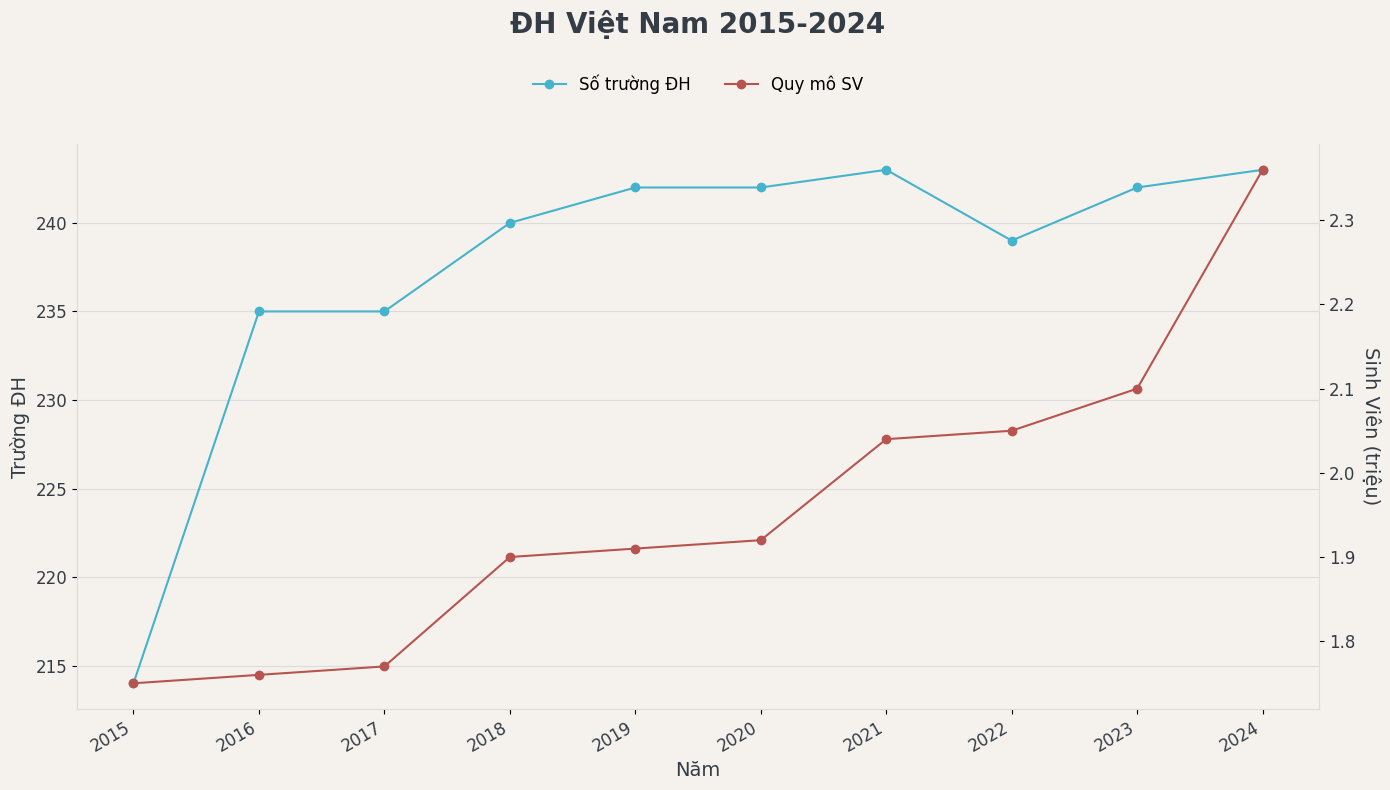
\includegraphics[width=0.9\textwidth]{bieu do 1 luan giao duc.png}} 
    \caption{Sự Tăng trưởng Quy mô Sinh viên và Số lượng Trường Đại học tại Việt Nam (2015-2024)}
    \label{fig:quy_mo_phat_trien}
    \vspace{0.2cm}
    \footnotesize{\textit{Nguồn: Tổng hợp từ dữ liệu của Bộ GD\&ĐT \cite{stat_moet_2024} và các báo cáo liên quan \cite{stat_quy_mo_2015_2021}.}}
\end{figure}



Đặc biệt, năm học 2023-2024 ghi nhận một sự tăng trưởng đột phá với \textbf{319.022} sinh viên tăng thêm so với năm học trước \cite{stat_moet_2024}. Đây không phải là một sự gia tăng tuyến tính thông thường mà là một \textbf{bước nhảy vọt (leap)} về quy mô, như được thể hiện rõ trên biểu đồ (Hình \ref{fig:quy_mo_phat_trien}). Sự gia tăng đột biến này không phải là một hiện tượng ngẫu nhiên, mà có thể được lý giải bởi sự hội tụ của nhiều yếu tố chính sách và xã hội diễn ra đồng thời, tạo ra một "cú hích" cho hệ thống.
\paragraph{Phân tích các nguyên nhân tiềm tàng:}
Một trong những nguyên nhân trực tiếp và quan trọng nhất có thể là sự thay đổi trong \textbf{chính sách tuyển sinh và việc gia tăng chỉ tiêu} của các trường đại học. Giai đoạn này chứng kiến sự phát triển mạnh mẽ của các phương thức xét tuyển đa dạng bên cạnh phương thức truyền thống dựa trên kết quả thi tốt nghiệp THPT. Việc các trường tăng cường sử dụng các phương thức như xét tuyển học bạ, kỳ thi đánh giá năng lực riêng đã mở ra nhiều "cửa" hơn cho thí sinh. Khi các trường đại học, đặc biệt là các trường ngoài công lập và các trường công lập tự chủ, được trao nhiều quyền tự chủ hơn trong việc xác định chỉ tiêu và phương thức tuyển sinh, họ có xu hướng mở rộng quy mô để đáp ứng nhu cầu xã hội và tối ưu hóa nguồn lực. Sự gia tăng chỉ tiêu trên toàn hệ thống, kết hợp với các phương thức xét tuyển linh hoạt, đã tạo điều kiện cho một số lượng lớn thí sinh trúng tuyển và nhập học hơn bao giờ hết.
Nguyên nhân thứ hai đến từ các \textbf{yếu tố kinh tế - xã hội và sự thay đổi trong nhận thức}. Giai đoạn sau đại dịch COVID-19 (2020-2022) đã có những tác động nhất định đến thị trường lao động và lựa chọn nghề nghiệp. Có thể một bộ phận không nhỏ học sinh và gia đình nhận thấy sự bấp bênh của thị trường lao động đối với những người không có trình độ chuyên môn cao, từ đó củng cố niềm tin rằng một tấm bằng đại học là "tấm vé bảo hiểm" cần thiết cho một tương lai ổn định. Áp lực "phổ cập hóa đại học" trong nhận thức xã hội đã thúc đẩy một tỷ lệ lớn hơn học sinh tốt nghiệp THPT quyết định theo đuổi con đường học vấn cao hơn, thay vì đi vào thị trường lao động hoặc các hệ thống giáo dục nghề nghiệp khác.
Cuối cùng, sự tăng trưởng đột biến này là kết quả của một \textbf{tác động cộng hưởng}. Các chính sách mở rộng tự chủ tuyển sinh của Bộ GD\&ĐT đã đóng vai trò như một "van xả" cho một "áp lực cầu" đã được tích tụ từ lâu trong xã hội. Khi cánh cửa đại học trở nên rộng mở hơn bao giờ hết, một lượng lớn nguyện vọng học tập của xã hội đã được hiện thực hóa trong cùng một năm học, tạo nên một bước nhảy vọt về quy mô.
Tuy nhiên, sự gia tăng nhanh chóng về quy mô này cũng chính là thách thức lớn nhất đối với công tác đảm bảo chất lượng. Nó đặt ra câu hỏi cấp bách về việc liệu sự phát triển của đội ngũ giảng viên, cơ sở vật chất, và đặc biệt là các quy trình quản lý chất lượng nội bộ có theo kịp tốc độ gia tăng của số lượng sinh viên hay không. Đây chính là bối cảnh thực tiễn đòi hỏi một hệ thống đảm bảo chất lượng bên ngoài phải hoạt động hiệu quả để vừa giám sát, vừa hỗ trợ các trường đại học vượt qua thách thức này.


\paragraph{Về cơ cấu sinh viên và vai trò của khối ngoài công lập:}
Sự phát triển của khối các trường đại học ngoài công lập là một điểm sáng trong việc xã hội hóa giáo dục. Tỷ lệ sinh viên theo học tại các trường ngoài công lập đã tăng dần, từ khoảng 20\% vào năm 2015 lên \textbf{22,76\%} vào năm 2024, với 536.295 sinh viên \cite{stat_moet_2024}. Con số này không chỉ cho thấy sự đóng góp ngày càng quan trọng của khu vực tư nhân mà còn cho thấy Việt Nam đã **vượt trước thời hạn mục tiêu 22,5\% sinh viên ngoài công lập vào năm 2025** được đề ra trong Nghị quyết 35 của Chính phủ. Sự lớn mạnh của khối ngoài công lập tạo ra một môi trường cạnh tranh lành mạnh, thúc đẩy các trường công lập phải không ngừng đổi mới và nâng cao chất lượng.

\subsubsection{Thực trạng Công tác Tuyển sinh và Xu hướng lựa chọn Ngành học}

Phân tích dữ liệu tuyển sinh không chỉ cho thấy bức tranh về đầu vào của hệ thống mà còn phản ánh xu hướng lựa chọn nghề nghiệp của thế hệ trẻ, một yếu tố quan trọng mà hệ thống ĐBCL cần phải nắm bắt để có những điều chỉnh phù hợp.

\paragraph{Tỷ lệ tham gia và kết quả tuyển sinh:}
Trong những năm gần đây, số lượng thí sinh tham gia kỳ thi tốt nghiệp THPT luôn duy trì ở mức ổn định trên 1 triệu \cite{stat_tuyen_sinh_2024_so_lieu, stat_thi_sinh_2024}. Đáng chú ý, tỷ lệ thí sinh đăng ký xét tuyển đại học chiếm một phần lớn, khoảng \textbf{68,5\%} tổng số thí sinh dự thi vào năm 2024, cho thấy nguyện vọng vào đại học vẫn là lựa chọn ưu tiên của đa số học sinh.

Tỷ lệ thí sinh xác nhận nhập học sau khi trúng tuyển là một chỉ số quan trọng phản ánh mức độ hấp dẫn và sự phù hợp của các chương trình đào tạo. Sau một giai đoạn sụt giảm nhẹ vào năm 2022 (80,34\%), tỷ lệ này đã phục hồi và đạt \textbf{81,87\%} vào năm 2024, với 551.497 thí sinh xác nhận nhập học \cite{stat_nhap_hoc_2024, stat_tuyen_sinh_2024_so_lieu}. 


% --- CHÈN BIỂU ĐỒ 2 ---
% --- CHÈN BIỂU ĐỒ (PHIÊN BẢN ĐÃ CẬP NHẬT) ---
\begin{figure}[h!]
    \centering
    % Thay thế bằng tên file ảnh mới bạn vừa tạo bằng Python
    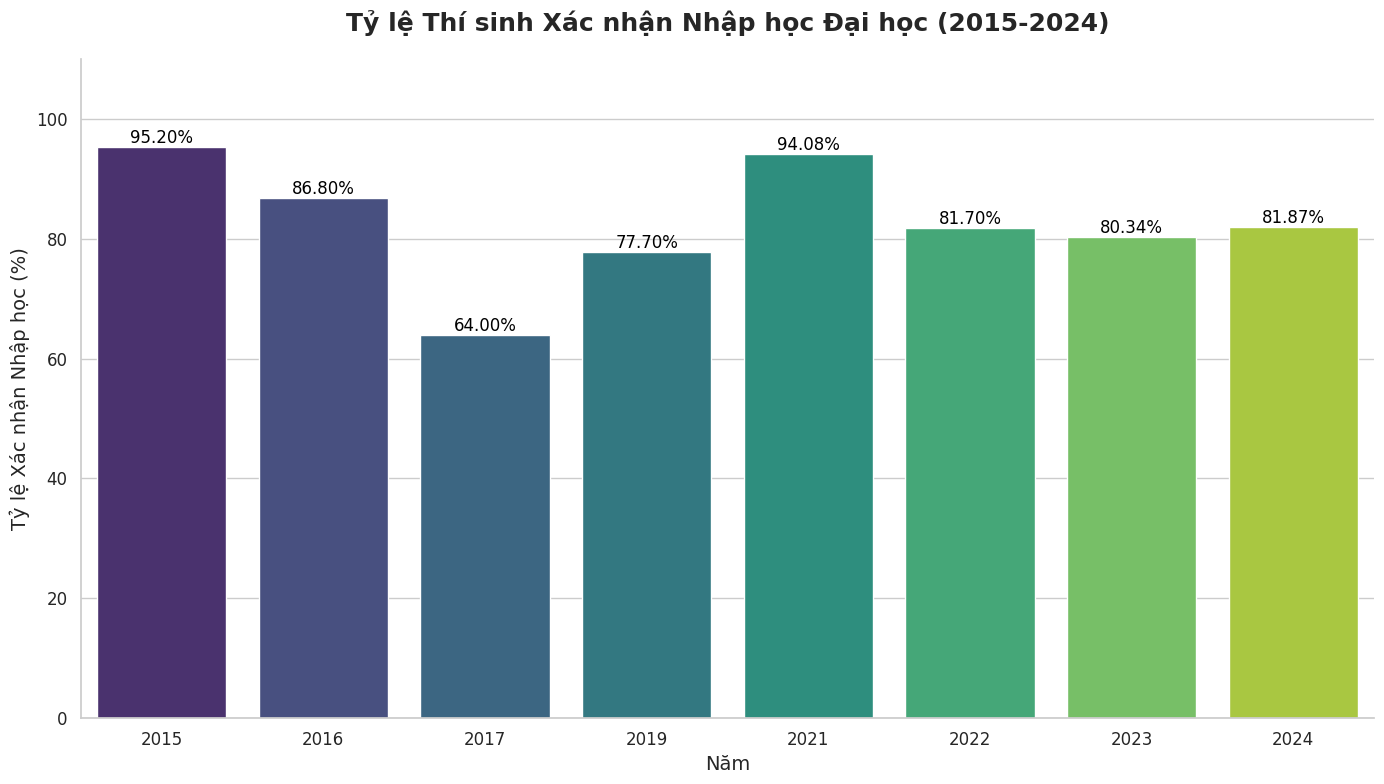
\includegraphics[width=0.8\textwidth]{ty_le_nhap_hoc_2015-2024.png}
    
    % Cập nhật caption cho đúng giai đoạn
    \caption{Tỷ lệ Thí sinh Xác nhận Nhập học Đại học (2015-2024)}
    \label{fig:ty_le_nhap_hoc_full}
    \vspace{0.2cm}
    
    % Cập nhật dòng nguồn với đầy đủ các trích dẫn
    \footnotesize{\textit{Nguồn: Tổng hợp từ dữ liệu của Bộ GD\&ĐT và các cơ quan báo chí qua các năm 
    \cite{ref1, ref2, ref3, ref5, ref7, ref12, ref19, stat_nhap_hoc_2024}.}}
\end{figure}


Điều này cho thấy niềm tin của xã hội vào hệ thống GDĐH đang được củng cố. Tỷ lệ nhập học cao cũng có nghĩa là trung bình cứ 100 học sinh dự thi tốt nghiệp THPT thì có khoảng 53 em vào đại học, đây là tỷ lệ cao nhất trong vòng 9 năm qua, khẳng định Việt Nam đã thực sự bước vào giai đoạn đại chúng hóa GDĐH \cite{stat_ty_le_vao_dh_2023}.

\paragraph{Xu hướng lựa chọn ngành học:}
Dữ liệu đăng ký xét tuyển năm 2024 cho thấy một sự thay đổi đáng kể trong xu hướng lựa chọn ngành nghề. Khối ngành **Khoa học giáo dục và Đào tạo giáo viên** bất ngờ có sự tăng trưởng vượt bậc với số lượng nguyện vọng tăng \textbf{85\%} so với năm 2023. Lĩnh vực Khoa học tự nhiên cũng thu hút sự quan tâm lớn với mức tăng 61% \cite{stat_tuyen_sinh_2024_so_lieu}.

Ngược lại, các khối ngành "nóng" trong những năm trước đây như **Kinh doanh và quản lý** (-3\%) và **Máy tính và Công nghệ thông tin** (-5\%) lại có xu hướng giảm nhẹ \cite{stat_tuyen_sinh_2024_so_lieu}. Sự dịch chuyển này có thể phản ánh sự thay đổi trong nhận thức về nhu cầu nhân lực dài hạn của xã hội và các chính sách mới của nhà nước đối với ngành giáo dục. Đây là một tín hiệu quan trọng mà các cơ quan ĐBCL và các trường đại học cần phân tích sâu để có những điều chỉnh kịp thời trong cơ cấu đào tạo.

\subsubsection{Phân tích Nguồn lực: Đội ngũ Giảng viên và Cơ sở vật chất}

Chất lượng của một hệ thống giáo dục phụ thuộc rất lớn vào chất lượng của đội ngũ giảng viên và các điều kiện đảm bảo.

\paragraph{Về đội ngũ giảng viên:}
Năm học 2023-2024, toàn hệ thống có \textbf{88.031 giảng viên cơ hữu}. Về trình độ, có \textbf{28.862 giảng viên có trình độ tiến sĩ (chiếm 32,8\%)}, 49.229 giảng viên có trình độ thạc sĩ (chiếm 55,9\%), và phần còn lại có trình độ đại học hoặc khác \cite{stat_moet_2024}. Cơ cấu trình độ này được minh họa trong Hình \ref{fig:co_cau_giang_vien}. Tỷ lệ giảng viên có trình độ tiến sĩ đã có sự cải thiện đáng kể so với những năm trước, đây là một tiền đề quan trọng để nâng cao chất lượng đào tạo và nghiên cứu.


% --- CHÈN BIỂU ĐỒ 3 ---
\begin{figure}[h!]
    \centering
    % Placeholder for the chart. Replace with your actual chart image.
    
\includegraphics[width=0.6\textwidth]{placeholder_chart_3.png}
    \caption{Cơ cấu Trình độ Đội ngũ Giảng viên Cơ hữu năm học 2023-2024}
    \label{fig:co_cau_giang_vien}
    \vspace{0.2cm}
    \footnotesize{\textit{Nguồn: Tính toán từ dữ liệu của Bộ GD\&ĐT \cite{stat_moet_2024}.}}
\end{figure}

Tuy nhiên, tỷ lệ sinh viên trên giảng viên vẫn còn ở mức cao, đặc biệt là ở các trường công lập. Tỷ lệ trung bình toàn quốc là 30 sinh viên/giảng viên ở trường công lập và 22 sinh viên/giảng viên ở trường ngoài công lập \cite{stat_moet_2024}. Tỷ lệ cao ở các trường công lập đặt ra thách thức lớn về việc đảm bảo sự tương tác hiệu quả giữa thầy và trò, một yếu tố cốt lõi của chất lượng giáo dục.

\paragraph{Về sự phân bố nguồn lực:}
Một thách thức lớn và cố hữu của hệ thống là sự mất cân đối nghiêm trọng trong phân bố địa lý. Các trường đại học và đội ngũ giảng viên chất lượng cao tập trung chủ yếu ở hai vùng kinh tế trọng điểm là Đồng bằng sông Hồng (44,3\% số trường) và Đông Nam Bộ (18,4\%). Trong khi đó, các vùng khó khăn như Tây Nguyên chỉ chiếm 1,6\% số trường \cite{stat_quy_mo_2015_2021, stat_phan_bo_dia_ly}. Sự mất cân bằng này cũng thể hiện rõ trong cơ hội tiếp cận GDĐH, khi tỷ lệ học sinh vào đại học ở Đồng bằng sông Hồng (64,44\%) cao hơn đáng kể so với vùng Trung du và miền núi phía Bắc (40,25\%) \cite{stat_ty_le_vao_dh_2023}. Sự chênh lệch này đòi hỏi các chính sách ĐBCL cần phải tính đến yếu tố vùng miền để đảm bảo sự phát triển công bằng và đồng đều.

\subsubsection{Phân tích Đầu ra: Tốt nghiệp và Việc làm}

Chất lượng đầu ra là thước đo cuối cùng và quan trọng nhất của một hệ thống giáo dục.
\begin{itemize}
    \item \textbf{Số lượng tốt nghiệp:} Năm 2024, hệ thống GDĐH đã cung cấp cho thị trường lao động **313.572 cử nhân, kỹ sư**, tăng mạnh so với con số 228.092 của năm 2023 \cite{stat_moet_2024}. Điều này cho thấy vai trò ngày càng quan trọng của GDĐH trong việc cung cấp nguồn nhân lực có trình độ cao.
    \item \textbf{Tình hình việc làm:} Tuy nhiên, chất lượng của nguồn nhân lực này vẫn là một dấu hỏi. Theo một báo cáo năm 2018, tỷ lệ sinh viên có việc làm sau khi tốt nghiệp chỉ đạt **65,5\%** \cite{stat_that_nghiep_2018}. Đáng lo ngại hơn, tỷ lệ thất nghiệp của nhóm có trình độ đại học, cao đẳng vẫn cao hơn so với nhóm có trình độ trung cấp. Điều này cho thấy một sự "không khớp" (mismatch) giữa kỹ năng được đào tạo và yêu cầu của thị trường lao động, một vấn đề cốt lõi mà hệ thống ĐBCL bên ngoài phải tập trung giải quyết.
\end{itemize}

\subsubsection{Kết luận sơ bộ về Thực trạng}
Phân tích các dữ liệu thống kê giai đoạn 2015-2024 cho thấy GDĐH Việt Nam đang trong một giai đoạn phát triển đầy năng động nhưng cũng tiềm ẩn nhiều thách thức.
\begin{itemize}
    \item \textbf{Thành tựu:} Quy mô đào tạo được mở rộng mạnh mẽ, đáp ứng nhu cầu học tập của xã hội; cơ cấu dịch chuyển tích cực sang khu vực ngoài công lập; trình độ đội ngũ giảng viên được cải thiện đáng kể.
    \item \textbf{Thách thức:} Sự tăng trưởng nóng về quy mô đặt ra áp lực lớn lên chất lượng; sự mất cân bằng về phân bố nguồn lực giữa các vùng miền vẫn còn sâu sắc; và quan trọng nhất, chất lượng đầu ra chưa thực sự đáp ứng được yêu cầu của thị trường lao động.
\end{itemize}
Những thách thức này khẳng định sự cần thiết phải có một hệ thống đảm bảo chất lượng bên ngoài mạnh mẽ, không chỉ để giám sát sự tuân thủ mà còn phải có khả năng thúc đẩy những thay đổi thực chất từ bên trong các cơ sở giáo dục, nhằm giải quyết các vấn đề cốt lõi về chất lượng và sự phù hợp.

%ket thuc goi 2


\section{Tổng quan Tình hình Nghiên cứu và Vấn đề Nghiên cứu}
\label{sec:tong_quan_nghien_cuu}

\subsection{Giới thiệu Tổng quan và Vấn đề Nghiên cứu}

Vấn đề chất lượng và đảm bảo chất lượng trong giáo dục đại học (GDĐH) Việt Nam, với những thách thức và cơ hội như đã phân tích ở trên, đã thu hút sự quan tâm của nhiều học giả, nhà quản lý và các tổ chức quốc tế trong những năm gần đây. Một khối lượng đáng kể các công trình nghiên cứu, báo cáo chính sách và các bài phân tích đã được công bố, tạo nên một nền tảng tri thức quan trọng về lĩnh vực này. Tuy nhiên, để một nghiên cứu mới có thể tạo ra đóng góp thực sự, việc hệ thống hóa và đánh giá một cách có phê phán các công trình đã có là một bước đi không thể thiếu. Quá trình tổng quan này không chỉ nhằm mục đích liệt kê những gì đã được thực hiện, mà quan trọng hơn, là để xác định những "vùng đất chưa được khám phá", những "câu hỏi còn bỏ ngỏ" — hay nói cách khác, là để xác định một cách rõ ràng \textbf{khoảng trống nghiên cứu (research gap)} mà luận án này hướng tới giải quyết.

Trên cơ sở đó, luận án này xác định vấn đề nghiên cứu trung tâm như sau:

\begin{center}
\textit{Sự thiếu hụt một hệ thống đảm bảo chất lượng (ĐBCL) bên ngoài đủ mạnh mẽ về mặt thể chế, đủ linh hoạt để thích ứng với bối cảnh thay đổi, và đủ toàn diện để dung hòa các yêu cầu đa dạng của các bên liên quan, đang tạo ra một rào cản mang tính hệ thống đối với mục tiêu nâng cao chất lượng thực chất và năng lực cạnh tranh quốc tế của nền giáo dục đại học Việt Nam.}
\end{center}

Để làm rõ hơn vấn đề này, phần tiếp theo sẽ tiến hành tổng quan các nghiên cứu liên quan theo hai nhóm chính: các nghiên cứu mang tầm quốc tế về các mô hình và lý thuyết ĐBCL, và các nghiên cứu tập trung cụ thể vào bối cảnh Việt Nam.

\subsection{Tổng quan các Nghiên cứu Quốc tế về Mô hình và Lý thuyết ĐBCL}

Nghiên cứu về ĐBCL GDĐH trên thế giới đã phát triển qua nhiều giai đoạn với các trọng tâm lý thuyết khác nhau, cung cấp những lăng kính phong phú để soi chiếu vào các hệ thống quốc gia.

Giai đoạn đầu, các nghiên cứu thường tập trung vào việc mô tả sự hình thành và cấu trúc của các cơ quan kiểm định, chủ yếu dưới góc độ quản lý công và chính sách công. Các công trình này nhấn mạnh vai trò của nhà nước trong việc thiết lập các quy tắc và giám sát hệ thống, một cách tiếp cận gần với Thuyết Ủy nhiệm \cite{Kivisto2008, DeBoer2019}. Trọng tâm là làm rõ mối quan hệ trách nhiệm giải trình giữa nhà nước và các trường đại học.

Bước sang một giai đoạn phát triển hơn, các nhà xã hội học tổ chức đã áp dụng Thuyết Tân Thể chế để lý giải tại sao các mô hình ĐBCL lại có xu hướng lan tỏa và trở nên đồng nhất trên toàn cầu. Các công trình của Meyer, Powell, DiMaggio đã trở thành kinh điển khi chỉ ra rằng các trường đại học không chỉ hành động dựa trên hiệu quả kỹ thuật mà còn chịu áp lực mạnh mẽ từ việc tìm kiếm tính hợp pháp trong môi trường thể chế \cite{MeyerPowell2020, DiMaggioPowell1983}. Các nghiên cứu sau này như của Kanwar và cộng sự (2019) đã vận dụng thành công khung lý thuyết này để phân tích các động lực thúc đẩy việc áp dụng ĐBCL trong các bối cảnh cụ thể \cite{Kanwar2019}.

Trong những năm gần đây, khi các hệ thống ĐBCL trở nên phức tạp hơn, các nhà nghiên cứu bắt đầu chú ý nhiều hơn đến sự tương tác giữa các chủ thể khác nhau. Thuyết Các bên Liên quan được vận dụng ngày càng nhiều để phân tích các mâu thuẫn lợi ích và sự cần thiết của việc thu hút các bên liên quan (đặc biệt là sinh viên và nhà tuyển dụng) vào quy trình ĐBCL. Các nghiên cứu như của Langrafe và cộng sự (2020) đã cung cấp bằng chứng thực nghiệm cho thấy sự tham gia của các bên liên quan có mối tương quan tích cực với việc tạo ra giá trị cho cả nhà trường và xã hội \cite{Langrafe2020}.

Đặc biệt, các nghiên cứu gần đây nhất đã nhận ra giới hạn của việc áp dụng các lý thuyết đơn lẻ và bắt đầu hướng tới các \textbf{mô hình tích hợp và lai ghép (hybrid models)}. Các báo cáo của Hiệp hội các trường Đại học Châu Âu (EUA) thường xuyên nhấn mạnh sự dịch chuyển từ mô hình "kiểm soát" sang mô hình "nâng cao chất lượng", trong đó các quy trình đánh giá bên ngoài được thiết kế để hỗ trợ và thúc đẩy các nỗ lực cải tiến từ bên trong \cite{EUA_Integration, HarveyStensaker}. Cách tiếp cận này công nhận rằng một hệ thống hiệu quả phải dung hòa được cả hai mục tiêu: trách nhiệm giải trình và cải tiến liên tục.

\textit{Bài học rút ra từ các nghiên cứu quốc tế:} Tổng quan các công trình quốc tế cho thấy một sự tiến hóa rõ rệt trong tư duy về ĐBCL—từ việc tập trung vào kiểm soát tuân thủ, đến việc lý giải các áp lực thể chế, và hiện nay là hướng tới các mô hình tích hợp, linh hoạt và có sự tham gia của nhiều bên. Điều này cho thấy rằng, việc phân tích hệ thống ĐBCL của một quốc gia như Việt Nam sẽ không đầy đủ nếu chỉ dựa vào các lý thuyết truyền thống hoặc chỉ mô tả các quy định chính sách. Một phân tích có chiều sâu cần phải đặt hệ thống của Việt Nam trong dòng chảy chung của các xu hướng lý thuyết và thực tiễn này, đồng thời nhận diện được những nét đặc thù của riêng mình.

%ket thuc goi 3


\subsection{Tổng quan Tình hình Nghiên cứu về ĐBCL GDĐH tại Việt Nam}
\label{subsec:tong_quan_vietnam}

Tại Việt Nam, vấn đề chất lượng và đảm bảo chất lượng GDĐH đã trở thành một chủ đề nhận được sự quan tâm lớn từ cả giới học thuật và các nhà hoạch định chính sách, đặc biệt là từ khi Luật Giáo dục Đại học được ban hành và sửa đổi. Các công trình nghiên cứu trong nước về lĩnh vực này khá phong phú và có thể được phân loại thành ba nhóm chính, mỗi nhóm có những đóng góp và cả những giới hạn riêng.

\paragraph{Nhóm 1: Các nghiên cứu về Lịch sử, Chính sách và Pháp luật.}
Đây là nhóm nghiên cứu phổ biến nhất, tập trung vào việc mô tả và hệ thống hóa quá trình phát triển của hệ thống GDĐH Việt Nam qua các thời kỳ. Các công trình của các tác giả như Lê Văn Giang (2003), hay các báo cáo tổng kết của Bộ GD\&ĐT qua các giai đoạn, đã cung cấp một cái nhìn toàn cảnh về sự thay đổi trong chủ trương, chính sách, từ thời kỳ bao cấp đến giai đoạn Đổi Mới và hội nhập \cite{LeVanGiang2003, MOET_50nam}. Các nghiên cứu này có giá trị cao về mặt tư liệu lịch sử, giúp hiểu rõ bối cảnh ra đời của các chính sách ĐBCL hiện hành. Tuy nhiên, hạn chế lớn của nhóm này là phương pháp tiếp cận chủ yếu là mô tả-thống kê. Chúng thường dừng lại ở việc "cái gì đã diễn ra" mà chưa đi sâu vào việc "tại sao nó lại diễn ra như vậy" dưới một lăng kính lý thuyết quản trị hiện đại. Do đó, chúng chưa lý giải được các động lực thể chế, các mâu thuẫn lợi ích, hay các vấn đề ủy nhiệm tiềm ẩn đằng sau các chính sách đó.

\paragraph{Nhóm 2: Các nghiên cứu về việc áp dụng các Mô hình Quản lý Chất lượng cụ thể.}
Nhóm thứ hai bao gồm các công trình nghiên cứu về việc ứng dụng các mô hình quản lý chất lượng cụ thể vào bối cảnh GDĐH. Nhiều tác giả như Trần Khánh Đức (2010), Nguyễn Đức Chính (2002) đã đi sâu vào các mô hình như Quản lý Chất lượng Toàn diện (Total Quality Management - TQM) hay các bộ tiêu chuẩn ISO \cite{TranKhanhDuc2010, NguyenDucChinh2002}. Các nghiên cứu này có giá trị thực tiễn cao, cung cấp những hướng dẫn chi tiết về cách thức triển khai một mô hình cụ thể tại một cơ sở giáo dục. Tuy nhiên, các công trình này thường mang tính "vi mô" hoặc "kỹ thuật". Chúng thường xem xét một mô hình quản lý một cách riêng lẻ mà chưa đặt nó trong mối quan hệ tương tác với toàn bộ hệ thống ĐBCL bên ngoài (với các trung tâm kiểm định, với chính sách của Bộ). Hơn nữa, chúng thường tập trung vào khía cạnh "làm thế nào để áp dụng" hơn là "tại sao mô hình này lại phù hợp hoặc không phù hợp với văn hóa tổ chức và bối cảnh thể chế của Việt Nam".

\paragraph{Nhóm 3: Các nghiên cứu về Thực trạng Kiểm định tại các Cơ sở Giáo dục.}
Nhóm thứ ba, phát triển mạnh mẽ trong những năm gần đây, tập trung vào việc phân tích thực trạng công tác kiểm định chất lượng tại các trường đại học cụ thể hoặc một nhóm trường. Các nghiên cứu này, thường được đăng tải trên các tạp chí chuyên ngành trong nước, đã chỉ ra rất nhiều khó khăn và thách thức thực tiễn mà các trường gặp phải, chẳng hạn như vấn đề về xây dựng đội ngũ, thu thập minh chứng, hay phát triển văn hóa chất lượng \cite{VJE_Challenges2023, ExpertPerspectivesVN}. Đây là những đóng góp vô cùng quý giá, cung cấp những bằng chứng thực chứng sinh động. Tuy nhiên, các nghiên cứu này thường mang tính "chẩn đoán" và phân tích tình huống (case study) đơn lẻ. Chúng chỉ ra rất rõ "triệu chứng" của vấn đề, nhưng thường chưa đi sâu phân tích "căn nguyên" mang tính hệ thống đã gây ra các triệu chứng đó. Chúng ta biết các trường gặp khó khăn về dữ liệu, nhưng tại sao vấn đề này lại mang tính phổ biến và hệ thống? Phải chăng nó xuất phát từ cấu trúc quản trị, từ mối quan hệ ủy nhiệm, hay từ các áp lực thể chế? Những câu hỏi này thường chưa được các nghiên cứu tình huống trả lời một cách thấu đáo.

\subsection{Xác định "Khoảng trống Nghiên cứu" và Hướng đi của Luận án}
\label{subsec:xac_dinh_khoang_trong}

Từ việc tổng quan một cách có hệ thống các dòng nghiên cứu trong và ngoài nước, một \textbf{khoảng trống nghiên cứu (research gap)} quan trọng đã được nhận diện rõ ràng. Cụ thể, các nghiên cứu tại Việt Nam, mặc dù phong phú, vẫn tồn tại ba hạn chế chính:
\begin{enumerate}
    \item \textbf{Thiếu vắng một khung lý thuyết tích hợp:} Hầu hết các nghiên cứu hiện có hoặc là mô tả chính sách thuần túy, hoặc áp dụng một mô hình kỹ thuật riêng lẻ. Rất hiếm có công trình nào sử dụng một cách có hệ thống các lý thuyết quản trị và tổ chức học hiện đại (như Thuyết Tân Thể chế, Thuyết Các bên Liên quan, Thuyết Ủy nhiệm) để phân tích một cách toàn diện hệ thống ĐBCL GDĐH Việt Nam. Điều này dẫn đến các phân tích thường chỉ dừng lại ở bề mặt mà chưa chạm đến các cấu trúc quyền lực và các động lực ngầm định hình hệ thống.
    
    \item \textbf{Thiếu một góc nhìn mang tính hệ thống:} Các nghiên cứu thường tập trung vào một chủ thể riêng lẻ (nhà nước, một trường đại học, một mô hình quản lý) mà chưa có một cái nhìn tổng thể, xem xét hệ thống ĐBCL như một hệ sinh thái phức tạp với sự tương tác động giữa nhiều chủ thể và nhiều tầng lớp khác nhau. Sự thiếu vắng góc nhìn hệ thống này khiến chúng ta khó lý giải được các "vòng luẩn quẩn" (vicious cycles) và các vấn đề mang tính hệ thống đã được các chuyên gia quốc tế chỉ ra.
    
    \item \textbf{Thiên về "chẩn đoán" hơn là "đề xuất mô hình":} Nhiều nghiên cứu đã chỉ ra rất thành công "căn bệnh" của hệ thống, nhưng lại chưa đưa ra được một "phác đồ điều trị" mang tính tổng thể, khả thi và được luận giải một cách chặt chẽ dựa trên nền tảng lý thuyết. Các giải pháp đề xuất thường mang tính chắp vá, giải quyết từng triệu chứng riêng lẻ thay vì một mô hình cải cách toàn diện.
\end{enumerate}

Chính việc nhận diện rõ ràng ba khoảng trống này đã định hình hướng đi và khẳng định tính mới của luận án. Luận án này được thực hiện không phải để lặp lại những gì đã có, mà là để trực tiếp lấp đầy những khoảng trống đó. Mục tiêu của luận án không chỉ là mô tả thực trạng, mà là \textbf{giải thích} thực trạng đó thông qua một khung lý thuyết tích hợp, và từ đó, \textbf{đề xuất} một mô hình cải cách có hệ thống và khả thi. Bằng cách xây dựng và vận dụng mô hình V-AQA, luận án sẽ cung cấp một góc nhìn mới, một công cụ phân tích mới, và một hướng tiếp cận mới cho vấn đề cải cách hệ thống đảm bảo chất lượng bên ngoài của giáo dục đại học Việt Nam trong giai đoạn phát triển và hội nhập sắp tới.


%ket thuc goi 4

\section{Mục tiêu, Câu hỏi và Ý nghĩa của Nghiên cứu}
\label{sec:muc_tieu_y_nghia}

Từ việc nhận diện "nghịch lý phát triển" của giáo dục đại học (GDĐH) Việt Nam và khoảng trống trong các nghiên cứu trước đây, luận án này được thực hiện với một mục tiêu rõ ràng, được cụ thể hóa thành các câu hỏi nghiên cứu sắc bén, và hướng tới những đóng góp có ý nghĩa cả về mặt lý luận và thực tiễn.

\subsection{Mục tiêu Nghiên cứu (Research Objectives)}
\label{subsec:muc_tieu_nghien_cuu}

Mục tiêu nghiên cứu của luận án là xác lập một cách có hệ thống những nền tảng lý thuyết và thực chứng để phân tích, đánh giá, và đề xuất các giải pháp khả thi nhằm hoàn thiện hệ thống đảm bảo chất lượng (ĐBCL) bên ngoài của GDĐH Việt Nam, góp phần giải quyết mâu thuẫn giữa tăng trưởng quy mô và yêu cầu nâng cao chất lượng trong bối cảnh hội nhập quốc tế.

Để thực hiện mục tiêu tổng quát đó, luận án sẽ tập trung vào bốn mục tiêu cụ thể sau:
\begin{enumerate}
    \item \textbf{Hệ thống hóa và xây dựng khung lý thuyết:} Phân tích phê phán các lý thuyết quản trị hiện đại (Tân Thể chế, Các bên Liên quan, Ủy nhiệm) và các mô hình ĐBCL tiên tiến trên thế giới, từ đó xây dựng một khung phân tích tích hợp—Mô hình V-AQA—phù hợp với bối cảnh đặc thù của Việt Nam.
    
    \item \textbf{Phân tích và "chẩn đoán" thực trạng:} Áp dụng khung lý thuyết V-AQA để phân tích một cách có hệ thống thực trạng hệ thống ĐBCL bên ngoài của Việt Nam, nhận diện các thành tựu, các thách thức cốt lõi, và những "điểm nghẽn" mang tính hệ thống đang cản trở sự phát triển.
    
    \item \textbf{Rút ra các bài học kinh nghiệm quốc tế:} Nghiên cứu so sánh sâu hai trường hợp điển hình là hệ thống ĐBCL của Trung Quốc và khung AUN-QA, từ đó rút ra những bài học kinh nghiệm có giá trị về việc cân bằng giữa kiểm soát và tự chủ, giữa tiêu chuẩn khu vực và bối cảnh quốc gia.
    
    \item \textbf{Đề xuất mô hình và giải pháp khả thi:} Dựa trên nền tảng lý thuyết và các phân tích thực chứng, đề xuất một cách chi tiết Mô hình ĐBCL Lai ghép và Thích ứng (V-AQA) như một giải pháp tổng thể, kèm theo một lộ trình triển khai và các kiến nghị chính sách cụ thể cho các nhà quản lý và hoạch định chính sách tại Việt Nam.
\end{enumerate}

\subsection{Câu hỏi Nghiên cứu (Research Questions)}
\label{subsec:cau_hoi_nghien_cuu}

Để định hướng cho quá trình nghiên cứu và đạt được các mục tiêu trên, luận án sẽ tập trung trả lời ba câu hỏi nghiên cứu chính sau đây:

\begin{enumerate}
    \item[\textbf{CQ1:}] \textbf{Hệ thống đảm bảo chất lượng bên ngoài của giáo dục đại học Việt Nam hiện nay đang vận hành với những đặc điểm, thành tựu và thách thức mang tính hệ thống nào?}
    \begin{itemize}
        \item \textit{Câu hỏi phụ 1a:} Các chủ thể chính (Bộ GD\&ĐT, các trung tâm kiểm định, các trường đại học) có vai trò và mối quan hệ tương tác như thế nào trong hệ thống?
        \item \textit{Câu hỏi phụ 1b:} Những "điểm nghẽn" cốt lõi nào (về quản trị, văn hóa, quy trình...) đang cản trở hiệu quả của hệ thống?
    \end{itemize}

    \item[\textbf{CQ2:}] \textbf{Kinh nghiệm từ mô hình ĐBCL của Trung Quốc và khung AUN-QA mang lại những bài học gì cho Việt Nam trong việc cân bằng giữa kiểm soát nhà nước và tự chủ đại học, giữa các tiêu chuẩn quốc tế/khu vực và bối cảnh quốc gia?}
    \begin{itemize}
        \item \textit{Câu hỏi phụ 2a:} Trung Quốc đã làm gì để vừa duy trì sự kiểm soát của nhà nước, vừa thúc đẩy năng lực cạnh tranh quốc tế, và Việt Nam có thể học hỏi điều gì từ sự cân bằng đó?
        \item \textit{Câu hỏi phụ 2b:} Việc áp dụng khung AUN-QA tại Việt Nam cho thấy những thuận lợi và thách thức nào trong việc hài hòa hóa các tiêu chuẩn khu vực vào hệ thống quốc gia?
    \end{itemize}

    \item[\textbf{CQ3:}] \textbf{Một mô hình đảm bảo chất lượng bên ngoài hiệu quả, phù hợp với bối cảnh Việt Nam cần có những cấu phần và đặc tính cốt lõi nào, và lộ trình triển khai ra sao?}
    \begin{itemize}
        \item \textit{Câu hỏi phụ 3a:} Các thành tố của một mô hình lai ghép và thích ứng (V-AQA) cần được thiết kế như thế nào để giải quyết các thách thức đã được nhận diện?
        \item \textit{Câu hỏi phụ 3b:} Những điều kiện tiên quyết và giải pháp chính sách nào cần có để triển khai thành công mô hình này trong thực tiễn?
    \end{itemize}
\end{enumerate}

\subsection{Ý nghĩa của Nghiên cứu (Significance of the Study)}
\label{subsec:y_nghia_nghien_cuu}

Việc trả lời các câu hỏi nghiên cứu trên sẽ mang lại những đóng góp có ý nghĩa quan trọng ở cả hai phương diện lý luận và thực tiễn.

\paragraph{Ý nghĩa về mặt Lý luận (Theoretical Significance):}
\begin{itemize}
    \item Luận án đóng góp vào kho tàng tri thức về quản trị GDĐH và ĐBCL bằng việc xây dựng và kiểm chứng một \textbf{khung phân tích lý thuyết tích hợp (V-AQA Model)}. Mô hình này vượt ra khỏi việc áp dụng các lý thuyết đơn lẻ, cung cấp một công cụ phân tích toàn diện hơn, đặc biệt hữu ích cho việc nghiên cứu các hệ thống GDĐH trong bối cảnh các quốc gia đang phát triển và chuyển đổi.
    \item Luận án làm phong phú thêm các nghiên cứu tình huống (case study) về ĐBCL GDĐH trên thế giới. Việc phân tích sâu và so sánh hệ thống của Việt Nam với Trung Quốc và AUN-QA sẽ cung cấp những dữ liệu và góc nhìn mới, góp phần vào sự hiểu biết chung của cộng đồng học thuật quốc tế về sự đa dạng và phức tạp của các mô hình ĐBCL.
\end{itemize}

\paragraph{Ý nghĩa về mặt Thực tiễn (Practical Significance):}
\begin{itemize}
    \item \textbf{Đối với các nhà hoạch định chính sách (Bộ GD\&ĐT):} Luận án cung cấp một bản "chẩn đoán" toàn diện về những điểm mạnh, điểm yếu và các vấn đề mang tính hệ thống của cơ chế ĐBCL hiện hành. Quan trọng hơn, các đề xuất và kiến nghị dựa trên mô hình V-AQA có thể trở thành một nguồn tham khảo hữu ích trong quá trình xây dựng và hoàn thiện các chính sách, thông tư, nghị định liên quan đến ĐBCL và tự chủ đại học trong giai đoạn tới.
    \item \textbf{Đối với các nhà quản lý giáo dục (lãnh đạo các trường đại học, các trung tâm kiểm định):} Luận án cung cấp một bộ công cụ tư duy và một khung hành động để các trường có thể tự soi chiếu, đánh giá hệ thống ĐBCL nội bộ của mình. Các phân tích về văn hóa chất lượng, quy trình nội bộ, hay sự tham gia của các bên liên quan sẽ giúp lãnh đạo nhà trường nhận diện các lĩnh vực cần ưu tiên cải tiến một cách có hệ thống thay vì các giải pháp tình thế.
    \item \textbf{Đối với cộng đồng học thuật và xã hội:} Luận án góp phần nâng cao nhận thức và thúc đẩy các cuộc thảo luận học thuật sâu rộng hơn về vấn đề chất lượng GDĐH tại Việt Nam, cung cấp những luận cứ khoa học cho các cuộc đối thoại chính sách, từ đó góp phần vào mục tiêu chung là xây dựng một nền GDĐH Việt Nam chất lượng và bền vững.
\end{itemize}


%ket thuc goi 5


\section{Đối tượng, Phạm vi và Luận điểm Nghiên cứu}
\label{sec:doi_tuong_pham_vi_luandiem}

Để đảm bảo tính khả thi, chiều sâu và sự tập trung của nghiên cứu, việc xác định rõ ràng đối tượng, phạm vi và công bố một luận điểm chính là điều kiện tiên quyết. Các yếu tố này sẽ định hình các giới hạn và trọng tâm của toàn bộ công trình.

\subsection{Đối tượng và Phạm vi Nghiên cứu (Object and Scope of the Study)}
\label{subsec:doi_tuong_pham_vi}

\paragraph{Đối tượng Nghiên cứu:}
Đối tượng nghiên cứu trọng tâm của luận án là \textbf{hệ thống đảm bảo chất lượng bên ngoài (External Quality Assurance - EQA) trong giáo dục đại học (GDĐH) tại Việt Nam}. Đối tượng này được hiểu là một hệ sinh thái phức hợp, bao gồm ba thành phần chính:
\begin{enumerate}
    \item \textbf{Các chủ thể (Actors):} Bao gồm các cơ quan hoạch định chính sách (chủ yếu là Bộ Giáo dục và Đào tạo), các tổ chức thực thi kiểm định (các trung tâm kiểm định chất lượng giáo dục trong nước và các tổ chức quốc tế/khu vực được cấp phép), và các cơ sở GDĐH (với tư cách là đối tượng chịu sự tác động của hệ thống).
    \item \textbf{Các cấu trúc và cơ chế (Structures and Mechanisms):} Bao gồm các văn bản pháp quy, các bộ tiêu chuẩn đánh giá, các quy trình kiểm định, và các cơ chế tài chính, chính sách có liên quan.
    \item \textbf{Các mối quan hệ tương tác (Interactions):} Bao gồm mối quan hệ quyền lực, trách nhiệm giải trình và hợp tác giữa các chủ thể nêu trên.
\end{enumerate}

\paragraph{Phạm vi Nghiên cứu:}
Để đảm bảo tính khả thi và chiều sâu, luận án giới hạn phạm vi nghiên cứu như sau:
\begin{itemize}
    \item \textbf{Về nội dung:} Nghiên cứu tập trung chủ yếu vào \textit{đảm bảo chất lượng bên ngoài (EQA)}. Các khía cạnh của đảm bảo chất lượng bên trong (Internal Quality Assurance - IQA) tại các trường đại học sẽ được đề cập, nhưng chủ yếu dưới góc độ là đối tượng chịu tác động và là một thành phần trong hệ thống EQA tổng thể, chứ không đi vào phân tích sâu từng quy trình IQA của một trường cụ thể.
    
    \item \textbf{Về thời gian:} Mặc dù có nhìn lại quá trình lịch sử, luận án sẽ tập trung phân tích các chính sách và thực tiễn trong giai đoạn từ năm \textbf{2012 đến nay}. Mốc 2012 được chọn vì đây là năm Luật Giáo dục Đại học lần đầu tiên được ban hành, đánh dấu một bước ngoặt quan trọng trong việc thể chế hóa hệ thống ĐBCL tại Việt Nam. Giai đoạn này cho phép nghiên cứu nắm bắt được những thay đổi và thách thức đương đại nhất của hệ thống.
    
    \item \textbf{Về không gian:} Nghiên cứu lấy bối cảnh \textbf{Việt Nam} làm trường hợp phân tích trung tâm (central case). Để có góc nhìn đối sánh và rút ra các bài học kinh nghiệm, luận án sẽ sử dụng hai trường hợp so sánh có chọn lọc: \textbf{hệ thống ĐBCL của Trung Quốc} (đại diện cho mô hình quốc gia do nhà nước dẫn dắt mạnh mẽ) và \textbf{khung AUN-QA} (đại diện cho mô hình hợp tác khu vực có ảnh hưởng trực tiếp đến Việt Nam).
\end{itemize}

\subsection{Luận điểm chính của Luận án (Thesis Statement)}
\label{subsec:luan_diem_chinh}

Dựa trên toàn bộ bối cảnh, khoảng trống nghiên cứu và mục tiêu đã xác định, luận án này sẽ bảo vệ và chứng minh cho luận điểm trung tâm sau đây:

\begin{quote}
\textit{\textbf{
Luận án này luận giải rằng, những thách thức cố hữu và mang tính hệ thống của hệ thống đảm bảo chất lượng bên ngoài trong giáo dục đại học Việt Nam—vốn thể hiện qua sự mâu thuẫn giữa tăng trưởng quy mô và trì trệ về chất lượng, giữa yêu cầu tự chủ và sự kiểm soát chặt chẽ—không thể được giải quyết bằng các giải pháp chính sách đơn lẻ hay việc áp dụng máy móc các mô hình quốc tế. Thay vào đó, chúng đòi hỏi một cách tiếp cận toàn diện, tích hợp và nhạy bén với bối cảnh.
}}

\textit{\textbf{
Do đó, luận án đề xuất và chứng minh rằng Mô hình Đảm bảo Chất lượng Lai ghép và Thích ứng (V-AQA), với năm thành tố cốt lõi là (1) Lãnh đạo \& Quản trị, (2) Văn hóa Chất lượng, (3) Sự tham gia của các Bên liên quan, (4) Quy trình Nội bộ, và (5) Hợp tác \& Phối hợp, là khung lý thuyết và giải pháp thực tiễn phù hợp nhất để tái cấu trúc hệ thống. Việc triển khai mô hình này có khả năng giải quyết các mâu thuẫn nội tại, thúc đẩy một văn hóa chất lượng tự thân, từ đó nâng cao chất lượng giáo dục đại học một cách bền vững và giúp Việt Nam hội nhập hiệu quả vào không gian giáo dục khu vực và thế giới.
}}
\end{quote}

Luận điểm này chính là sợi chỉ đỏ xuyên suốt, là linh hồn của toàn bộ công trình nghiên cứu. Các chương tiếp theo của luận án, từ phân tích thực trạng, so sánh quốc tế đến đề xuất giải pháp, đều sẽ được triển khai nhằm mục đích cung cấp các luận cứ lý thuyết và thực chứng để bảo vệ cho luận điểm trung tâm này.

% ket thuc goi 6

\section{Phương pháp luận và Phương pháp Nghiên cứu}
\label{sec:phuong_phap_luan}

Để trả lời các câu hỏi nghiên cứu đã đặt ra và kiểm chứng cho luận điểm trung tâm, luận án này áp dụng một phương pháp luận được thiết kế một cách có hệ thống, kết hợp nhiều phương pháp nghiên cứu cụ thể. Phần này sẽ trình bày chi tiết về triết lý nghiên cứu, cách tiếp cận, thiết kế nghiên cứu tổng thể, và các phương pháp thu thập, phân tích dữ liệu sẽ được sử dụng.

\subsection{Triết lý và Tiếp cận Nghiên cứu (Research Philosophy and Approach)}
\label{subsec:triet_ly_tiep_can}

Mỗi công trình nghiên cứu khoa học đều được định hướng bởi một hệ thống các giả định nền tảng về bản chất của thực tại (bản thể luận - ontology) và bản chất của tri thức (nhận thức luận - epistemology). Việc làm rõ các giả định này giúp xác định phương pháp tiếp cận phù hợp và đảm bảo tính nhất quán của toàn bộ nghiên cứu \cite{Creswell2018}.

Luận án này được thực hiện dựa trên nền tảng triết lý của \textbf{Chủ nghĩa Kiến tạo (Constructivism)}. Triết lý này cho rằng thực tại xã hội không phải là một cái gì đó khách quan, tồn tại độc lập bên ngoài, mà được "kiến tạo" (constructed) thông qua sự tương tác, diễn giải và các ý nghĩa mà con người gán cho nó \cite{GubaLincoln1994}. Áp dụng vào đề tài này, "chất lượng giáo dục" hay "hiệu quả của một hệ thống đảm bảo chất lượng" không phải là một sự thật duy nhất, khách quan, mà là một khái niệm phức hợp, được định hình bởi các góc nhìn, lợi ích và sự tương tác của nhiều chủ thể khác nhau (nhà nước, nhà trường, sinh viên, doanh nghiệp). Vì vậy, để hiểu được hệ thống ĐBCL, nghiên cứu cần phải đi sâu vào việc tìm hiểu các bối cảnh, các quy trình và các diễn giải đa dạng của các chủ thể trong hệ thống đó.

Từ nền tảng triết lý này, luận án áp dụng một \textbf{cách tiếp cận định tính (qualitative approach)} làm chủ đạo. Cách tiếp cận định tính đặc biệt phù hợp với đề tài này vì những lý do sau:
\begin{itemize}
    \item \textbf{Khám phá chiều sâu và sự phức tạp:} Các vấn đề về chính sách, quản trị, và văn hóa tổ chức trong ĐBCL là những vấn đề phức tạp, đa chiều, không thể dễ dàng lượng hóa. Phương pháp định tính cho phép nhà nghiên cứu đi sâu vào bản chất của vấn đề, khám phá các mối quan hệ nhân quả tinh vi và các yếu tố bối cảnh đặc thù \cite{Yin2018}.
    \item \textbf{Lý giải ý nghĩa và diễn giải:} Thay vì chỉ đo lường "cái gì" đang xảy ra, nghiên cứu định tính tập trung vào việc lý giải "tại sao" và "như thế nào". Nó cho phép phân tích các diễn giải, các quan điểm và các động lực của các chủ thể khác nhau, vốn là yếu tố cốt lõi để hiểu được sự vận hành của một hệ thống xã hội.
    \item \textbf{Xây dựng lý thuyết từ thực tiễn:} Cách tiếp cận này rất phù hợp với mục tiêu của luận án là không chỉ kiểm chứng mà còn xây dựng mô hình lý thuyết mới (V-AQA). Thông qua việc phân tích sâu các dữ liệu thực tiễn, nghiên cứu có thể rút ra các khái niệm, các mối quan hệ và xây dựng nên một khung lý thuyết có cơ sở vững chắc từ thực tiễn (grounded theory approach) \cite{Charmaz2006}.
\end{itemize}

\subsection{Thiết kế Nghiên cứu (Research Design)}
\label{subsec:thiet_ke_nghien_cuu}

Để hiện thực hóa cách tiếp cận định tính, luận án sử dụng một \textbf{thiết kế nghiên cứu tình huống so sánh (comparative case study design)}. Thiết kế này được lựa chọn vì nó cho phép nhà nghiên cứu thực hiện một cuộc điều tra sâu rộng, mang tính thực chứng về một hiện tượng đương đại trong bối cảnh thực của nó, đặc biệt là khi ranh giới giữa hiện tượng và bối cảnh không rõ ràng \cite{Yin2018}.

Trong thiết kế này, các "tình huống" (cases) được lựa chọn một cách có chủ đích để phục vụ cho mục tiêu nghiên cứu, cụ thể như sau:
\begin{itemize}
    \item \textbf{Tình huống chính, nghiên cứu chiều sâu (In-depth, Primary Case): Hệ thống ĐBCL bên ngoài của Việt Nam.} Đây là trọng tâm của toàn bộ luận án. Việc nghiên cứu sâu tình huống này nhằm mục đích "chẩn đoán" một cách toàn diện thực trạng, các động lực, thách thức và các mối quan hệ phức tạp giữa các chủ thể.
    
    \item \textbf{Các tình huống so sánh (Comparative Cases):}
    \begin{enumerate}
        \item \textbf{Hệ thống ĐBCL của Trung Quốc:} Được chọn làm tình huống so sánh vì nó đại diện cho một mô hình "nhà nước mạnh", tập trung, có nhiều điểm tương đồng về mặt cấu trúc chính trị-xã hội với Việt Nam nhưng lại ở một quy mô và mức độ phát triển khác. Việc so sánh với Trung Quốc giúp rút ra các bài học về việc cân bằng giữa kiểm soát và cạnh tranh.
        \item \textbf{Khung ĐBCL của AUN-QA:} Được chọn vì đây là mô hình khu vực có ảnh hưởng trực tiếp và mạnh mẽ nhất đến Việt Nam. Nó đại diện cho một cách tiếp cận dựa trên mạng lưới, hợp tác ngang hàng, trái ngược với mô hình tập trung của nhà nước. Việc phân tích AUN-QA giúp rút ra các bài học về hài hòa hóa tiêu chuẩn và hội nhập khu vực.
    \end{enumerate}
\end{itemize}

Việc sử dụng thiết kế so sánh đa tình huống (multiple-case study) mang lại nhiều lợi thế. Nó không chỉ giúp làm rõ các đặc điểm riêng của tình huống chính (Việt Nam) mà còn cho phép nhà nghiên cứu đưa ra các kết luận có tính khái quát hóa phân tích (analytic generalization) cao hơn, thay vì chỉ là các kết luận giới hạn trong một bối cảnh duy nhất \cite{Yin2018}.

Quá trình nghiên cứu sẽ được triển khai theo các giai đoạn logic sau:
\begin{enumerate}
    \item \textbf{Giai đoạn 1: Xây dựng Khung lý thuyết.} Đây chính là nội dung của Chương 2, nơi mô hình phân tích V-AQA được thiết lập.
    \item \textbf{Giai đoạn 2: Thu thập và Phân tích Dữ liệu cho từng Tình huống.} Sử dụng các phương pháp cụ thể (sẽ trình bày ở phần sau) để thu thập và phân tích dữ liệu cho từng tình huống (Việt Nam, Trung Quốc, AUN-QA).
    \item \textbf{Giai đoạn 3: Phân tích So sánh Chéo (Cross-case Analysis).} Đối chiếu và so sánh các phát hiện từ ba tình huống dựa trên khung phân tích V-AQA, từ đó xác định các điểm tương đồng, khác biệt và rút ra các bài học kinh nghiệm.
    \item \textbf{Giai đoạn 4: Tổng hợp và Đề xuất Mô hình.} Dựa trên toàn bộ kết quả phân tích, hoàn thiện và đề xuất chi tiết mô hình V-AQA như một giải pháp khả thi cho Việt Nam.
\end{enumerate}

Thiết kế nghiên cứu này đảm bảo sự chặt chẽ và logic, cho phép luận án đi từ lý thuyết đến thực tiễn, từ phân tích đến đề xuất một cách có hệ thống và thuyết phục.

% ket thuc goi 7
\subsection{Các Phương pháp Thu thập và Phân tích Dữ liệu}
\label{subsec:phuong_phap_cu_the}

Để thực hiện thiết kế nghiên cứu tình huống so sánh đã đề ra, luận án sẽ chủ yếu dựa vào việc thu thập và phân tích dữ liệu thứ cấp (secondary data) thông qua các phương pháp nghiên cứu định tính. Sự kết hợp của nhiều phương pháp sẽ giúp tăng cường tính hợp lệ và độ tin cậy của các kết quả nghiên cứu (triangulation) \cite{DenzinLincoln2011}.

\subsubsection{Phương pháp Phân tích Tài liệu (Documentary Analysis)}
\label{subsubsec:phan_tich_tai_lieu}

Đây là phương pháp thu thập và phân tích dữ liệu \textbf{chủ đạo và quan trọng nhất} của luận án. Phân tích tài liệu là một quy trình có hệ thống để xem xét và đánh giá các tài liệu, cả bản in và bản điện tử, nhằm rút ra các ý nghĩa, thu thập thông tin và tạo ra các bằng chứng thực chứng \cite{Bowen2009}. Phương pháp này đặc biệt phù hợp vì nó cho phép tiếp cận một nguồn dữ liệu phong phú, ổn định và không có tính phản ứng (non-reactive), giúp nhà nghiên cứu có thể phân tích các chính sách và thực tiễn mà không làm ảnh hưởng đến đối tượng được nghiên cứu.

Các nguồn tài liệu chính sẽ được thu thập và phân tích bao gồm ba nhóm:
\begin{enumerate}
    \item \textbf{Nhóm tài liệu Pháp quy và Chính sách:} Đây là các văn bản chính thức, cung cấp khung pháp lý cho hệ thống ĐBCL.
    \begin{itemize}
        \item \textit{Ví dụ tại Việt Nam:} Luật Giáo dục (2019), Luật Giáo dục Đại học (2012) và Luật sửa đổi, bổ sung (2018); các Nghị định của Chính phủ; các Thông tư và Quyết định của Bộ GD\&ĐT liên quan đến việc ban hành chuẩn chương trình, tiêu chuẩn đánh giá chất lượng, và quy định về tổ chức, hoạt động của các trung tâm kiểm định.
        \item \textit{Ví dụ tại Trung Quốc và AUN-QA:} Các văn bản tương ứng của Bộ Giáo dục Trung Quốc, các tài liệu hướng dẫn chính thức của AUN-QA (Guide to AUN-QA Assessment).
    \end{itemize}
    
    \item \textbf{Nhóm tài liệu Báo cáo và Đánh giá:} Đây là các tài liệu "sống", phản ánh thực tiễn hoạt động của hệ thống.
    \begin{itemize}
        \item Báo cáo tự đánh giá (Self-Assessment Reports - SAR) của một số trường đại học tiêu biểu tại Việt Nam khi tham gia kiểm định.
        \item Báo cáo đánh giá ngoài (External Assessment Reports) của các trung tâm kiểm định đối với các trường đại học.
        \item Các báo cáo phân tích, đánh giá của các tổ chức quốc tế như Ngân hàng Thế giới (World Bank), Ngân hàng Phát triển Châu Á (ADB), và các tổ chức hợp tác phát triển khác (British Council).
        \item Báo cáo tổng kết năm học, các đề án, chiến lược phát triển của Bộ GD\&ĐT và các trường đại học.
    \end{itemize}
    
    \item \textbf{Nhóm tài liệu Học thuật và Lưu trữ:} Bao gồm các công trình nghiên cứu đã được công bố.
    \begin{itemize}
        \item Các bài báo khoa học trên các tạp chí chuyên ngành trong nước và quốc tế.
        \item Các kỷ yếu hội thảo quốc gia và quốc tế về ĐBCL GDĐH.
        \item Các luận án, luận văn có liên quan đã được bảo vệ.
        \item Các bài phân tích, bình luận chính sách trên các phương tiện truyền thông uy tín.
    \end{itemize}
\end{enumerate}

Quá trình phân tích sẽ được thực hiện theo phương pháp \textbf{phân tích nội dung chuyên đề (thematic content analysis)}. Dữ liệu từ các tài liệu sẽ được mã hóa, phân loại và sắp xếp theo các chủ đề được định sẵn bởi năm thành tố của khung lý thuyết V-AQA (Lãnh đạo \& Quản trị, Văn hóa Chất lượng, v.v.). Cách tiếp cận này giúp đảm bảo việc phân tích dữ liệu được thực hiện một cách có hệ thống và trực tiếp phục vụ cho việc trả lời các câu hỏi nghiên cứu \cite{BraunClarke2006}.

\subsubsection{Phương pháp Lịch sử (Historical Analysis)}
\label{subsubsec:phan_tich_lich_su}
Phương pháp lịch sử sẽ được sử dụng để tái dựng lại quá trình tiến hóa của hệ thống ĐBCL bên ngoài tại Việt Nam. Nó không chỉ đơn thuần là việc kể lại các sự kiện theo trình tự thời gian, mà là một nỗ lực nhằm lý giải sự thay đổi và tính liên tục của các chính sách trong bối cảnh lịch sử-xã hội cụ thể \cite{Tosh2015}. Bằng cách phân tích các chính sách ĐBCL từ giai đoạn Đổi Mới đến nay, phương pháp này sẽ giúp trả lời các câu hỏi như:
\begin{itemize}
    \item Tại sao một chính sách cụ thể lại ra đời vào thời điểm đó?
    \item Những yếu tố kinh tế, chính trị, xã hội nào đã tác động đến sự thay đổi của hệ thống ĐBCL?
    \item Các chính sách cũ đã để lại những "di sản" (legacies) nào ảnh hưởng đến hệ thống hiện tại?
\end{itemize}
Việc áp dụng phương pháp này giúp nghiên cứu có một chiều sâu lịch sử, tránh được cái nhìn tĩnh tại và phi bối cảnh về hệ thống ĐBCL.

\subsubsection{Phương pháp So sánh (Comparative Analysis)}
\label{subsubsec:phan_tich_so_sanh}
Như đã trình bày trong thiết kế nghiên cứu, phương pháp so sánh đóng một vai trò trung tâm. Đây không phải là một sự so sánh tùy tiện, mà là một sự đối chiếu có hệ thống, có mục đích dựa trên một khung phân tích rõ ràng \cite{Sartori1991}.
\begin{itemize}
    \item \textbf{Mục đích so sánh:} Không phải để xếp hạng hệ thống nào "tốt hơn", mà để: (1) Làm nổi bật những đặc điểm độc đáo và riêng biệt của hệ thống Việt Nam (thông qua đối chiếu với các hệ thống khác); (2) Rút ra các bài học kinh nghiệm khả thi và các nguyên tắc chung có thể áp dụng được cho bối cảnh Việt Nam.
    \item \textbf{Khung so sánh:} Để tránh một sự so sánh hời hợt, luận án sẽ sử dụng chính \textbf{mô hình V-AQA với năm thành tố} làm khung để đối chiếu. Ví dụ, chương so sánh sẽ phân tích: Thành tố \textit{Lãnh đạo \& Quản trị} ở Việt Nam khác gì so với Trung Quốc? Thành tố \textit{Quy trình Nội bộ} của Việt Nam có thể học hỏi gì từ khung AUN-QA?
    \item \textbf{Logic so sánh:} Luận án sẽ áp dụng logic "hệ thống tương đồng, kết quả khác biệt" (most similar systems, different outcomes) và "hệ thống khác biệt, kết quả tương đồng" (most different systems, similar outcomes) để tìm ra các yếu tố giải thích quan trọng \cite{PrzeworskiTeune1970}.
\end{itemize}

\subsubsection{Phương pháp Tổng hợp Lý thuyết và Xây dựng Mô hình (Model Building)}
\label{subsubsec:xay_dung_mo_hinh}
Đây là một phương pháp mang tính sáng tạo, thể hiện đóng góp cốt lõi của luận án. Nó bao gồm các bước:
\begin{enumerate}
    \item Phê phán và chỉ ra giới hạn của các lý thuyết hiện có.
    \item Tổng hợp các khái niệm và các mối quan hệ quan trọng từ các lý thuyết khác nhau.
    \item Xây dựng một mô hình mới (V-AQA) với các cấu phần và mối liên kết được định nghĩa rõ ràng.
    \item Vận dụng mô hình đó để phân tích dữ liệu thực tiễn và kiểm chứng tính hữu dụng của nó.
\end{enumerate}
Phương pháp này giúp luận án không chỉ là người "tiêu thụ" lý thuyết mà còn là người "tạo ra" một công cụ lý thuyết mới, dù ở quy mô hẹp, góp phần vào sự phát triển của lĩnh vực nghiên cứu.

Sự kết hợp nhuần nhuyễn của bốn phương pháp này sẽ đảm bảo rằng luận án có thể trả lời các câu hỏi nghiên cứu một cách toàn diện, với các lập luận được củng cố bởi cả chiều sâu lý thuyết và sự phong phú của bằng chứng thực chứng.

% ket thuc goi 8

\section{Các Khái niệm Cốt lõi}
\label{sec:khai_niem_cot_loi}

Để đảm bảo sự rõ ràng, nhất quán và chính xác trong toàn bộ luận án, việc định nghĩa một cách tường minh các khái niệm cốt lõi là một yêu cầu bắt buộc. Phần này sẽ tập trung làm rõ các thuật ngữ trung tâm sẽ được sử dụng xuyên suốt, bao gồm: "Chất lượng trong GDĐH", "Đảm bảo chất lượng", và mối quan hệ giữa "Đảm bảo chất lượng bên ngoài" và "Kiểm định".

\subsection{Chất lượng trong Giáo dục Đại học: Một Khái niệm Đa chiều}
\label{subsec:khai_niem_chat_luong}

"Chất lượng" là một trong những khái niệm được tranh luận nhiều nhất và cũng khó nắm bắt nhất trong nghiên cứu về GDĐH. Nó không phải là một khái niệm đơn nhất, tĩnh tại, mà mang tính đa chiều, phụ thuộc vào bối cảnh và góc nhìn của các bên liên quan khác nhau. Harvey và Green (1993) trong một công trình kinh điển đã xác định năm cách tiếp cận khác nhau để định nghĩa chất lượng, giúp làm sáng tỏ sự phức tạp của khái niệm này \cite{HarveyGreen1993}:

\begin{enumerate}
    \item \textbf{Chất lượng như là sự ngoại lệ (Quality as Exceptional):} Đây là quan điểm truyền thống, coi chất lượng là một thứ gì đó đặc biệt, cao cấp, chỉ có ở một số ít các cơ sở giáo dục ưu tú. Theo cách nhìn này, chất lượng đồng nghĩa với việc vượt qua các tiêu chuẩn cao nhất và khó có thể đạt được một cách rộng rãi.
    
    \item \textbf{Chất lượng như là sự hoàn hảo (Quality as Perfection or Consistency):} Quan điểm này, chịu ảnh hưởng từ lĩnh vực sản xuất công nghiệp, định nghĩa chất lượng là "không có lỗi" (zero defects) và đáp ứng một cách nhất quán các thông số kỹ thuật đã được đặt ra. Nó nhấn mạnh vào quy trình và sự tuân thủ.
    
    \item \textbf{Chất lượng như là sự phù hợp với mục tiêu (Quality as Fitness for Purpose):} Đây là một trong những định nghĩa có ảnh hưởng nhất. Chất lượng được đánh giá dựa trên mức độ một cơ sở giáo dục hay một chương trình đào tạo đạt được các mục tiêu và sứ mệnh mà nó đã tự công bố. Một trường dạy nghề có thể có chất lượng cao nếu nó thực hiện xuất sắc mục tiêu đào tạo ra những người thợ lành nghề, ngay cả khi nó không phải là một viện nghiên cứu hàng đầu.
    
    \item \textbf{Chất lượng như là giá trị đồng tiền (Quality as Value for Money):} Từ góc độ của người chi trả (chính phủ, phụ huynh, sinh viên), chất lượng được xem xét dưới lăng kính của hiệu quả đầu tư. Một chương trình chất lượng là chương trình mang lại lợi ích (ví dụ: cơ hội việc làm, thu nhập cao) tương xứng hoặc lớn hơn chi phí đã bỏ ra. Cách tiếp cận này nhấn mạnh đến trách nhiệm giải trình về tài chính.
    
    \item \textbf{Chất lượng như là sự chuyển hóa (Quality as Transformation):} Đây là một quan điểm mang tính giáo dục sâu sắc, tập trung vào người học. Chất lượng được định nghĩa là khả năng của quá trình giáo dục trong việc tạo ra sự thay đổi, sự chuyển hóa tích cực cho người học—không chỉ về kiến thức, kỹ năng mà còn về tư duy, nhận thức và giá trị. Đây là quá trình "tạo ra giá trị gia tăng" (value-added) cho sinh viên.
\end{enumerate}

Nhận thức được tính đa chiều này, luận án này sẽ không chọn một định nghĩa duy nhất mà áp dụng một \textbf{quan điểm tổng hợp}. Theo đó, \textbf{chất lượng trong GDĐH} được hiểu là khả năng của một cơ sở giáo dục trong việc: \textit{(1) Đạt được các mục tiêu đã công bố và các tiêu chuẩn tối thiểu đã cam kết (phù hợp với mục tiêu); (2) Đáp ứng và tạo ra giá trị cho các bên liên quan chính, đặc biệt là người học và xã hội (sự chuyển hóa và giá trị đồng tiền); và (3) Liên tục cải tiến các quy trình để duy trì và nâng cao các giá trị đó một cách bền vững.}

\subsection{Đảm bảo Chất lượng và Kiểm định: Phân biệt và Mối quan hệ}
\label{subsec:khai_niem_dbcl_kd}

Trong các thảo luận về chất lượng, hai thuật ngữ "Đảm bảo chất lượng" (Quality Assurance - QA) và "Kiểm định" (Accreditation) thường được sử dụng thay thế cho nhau, nhưng thực chất chúng có ý nghĩa khác nhau và có mối quan hệ bao hàm.

\paragraph{Đảm bảo Chất lượng (Quality Assurance - QA):}
Đảm bảo chất lượng là một khái niệm rộng hơn, mang tính quy trình và hệ thống. Theo định nghĩa của Mạng lưới Quốc tế các Cơ quan Đảm bảo Chất lượng trong Giáo dục Đại học (INQAAHE), ĐBCL là "tất cả các chính sách, quy trình, hành động có kế hoạch và hệ thống cần thiết để tạo ra sự tin tưởng rằng chất lượng đang được duy trì và nâng cao" \cite{INQAAHE_Glossary}.
Như vậy, ĐBCL bao gồm tất cả các hoạt động mà một trường đại học thực hiện để quản lý chất lượng của mình, từ việc thiết kế chương trình, tuyển sinh, giảng dạy, đánh giá sinh viên, đến việc thu thập phản hồi và thực hiện cải tiến. Nó có cả hai khía cạnh:
\begin{itemize}
    \item \textbf{Đảm bảo chất lượng bên trong (Internal Quality Assurance - IQA):} Là toàn bộ các cơ chế và quy trình do chính cơ sở giáo dục thiết lập và vận hành để tự giám sát và cải tiến chất lượng của mình.
    \item \textbf{Đảm bảo chất lượng bên ngoài (External Quality Assurance - EQA):} Là các hoạt động được thực hiện bởi một cơ quan bên ngoài (ví dụ: cơ quan kiểm định, cơ quan của chính phủ) để đánh giá và xác nhận chất lượng của một cơ sở giáo dục hoặc một chương trình đào tạo.
\end{itemize}

\paragraph{Kiểm định (Accreditation):}
Kiểm định là một \textbf{hình thức cụ thể} và \textbf{chính thức} của ĐBCL bên ngoài. Nó được định nghĩa là "một quy trình đánh giá đồng cấp (peer review) nhằm xác định xem một cơ sở giáo dục hoặc một chương trình đào tạo có đáp ứng các tiêu chuẩn chất lượng đã được xác định trước hay không" \cite{CHEA_Definition}. Kết quả của quá trình kiểm định thường là một quyết định "công nhận" hoặc "không công nhận", có giá trị trong một khoảng thời gian nhất định. Kiểm định có hai mục đích chính: đảm bảo chất lượng và thúc đẩy cải tiến chất lượng.

\paragraph{Mối quan hệ:}
Mối quan hệ giữa hai khái niệm này có thể được hình dung như sau: \textbf{Kiểm định là một trong những công cụ quan trọng và phổ biến nhất của hệ thống Đảm bảo chất lượng bên ngoài}. Hệ thống EQA là một khái niệm bao trùm, ngoài kiểm định, nó có thể bao gồm các hoạt động khác như đánh giá (assessment), xếp hạng (ranking), hoặc cấp phép hoạt động (licensing).

Trong khuôn khổ của luận án này, khi đề cập đến \textbf{"hệ thống đảm bảo chất lượng bên ngoài"}, chúng tôi muốn nói đến toàn bộ hệ sinh thái EQA tại Việt Nam, bao gồm các chính sách, các cơ quan và các cơ chế liên quan. Trong đó, \textbf{"hoạt động kiểm định chất lượng"} sẽ được xem xét như là một công cụ trung tâm và là biểu hiện rõ nét nhất của hệ thống EQA đó. Việc phân biệt rõ ràng hai khái niệm này giúp tránh được sự nhầm lẫn và cho phép phân tích các chính sách và thực tiễn một cách chính xác hơn.

% ket thuc goi 9

\section{Cấu trúc của Luận án (Structure of the Dissertation)}
\label{sec:cau_truc_luan_an}

Để trả lời các câu hỏi nghiên cứu và bảo vệ cho luận điểm trung tâm đã được trình bày, luận án được cấu trúc một cách logic thành năm chương chính, không bao gồm phần mở đầu và kết luận chung. Mỗi chương giải quyết một mục tiêu nghiên cứu cụ thể và xây dựng nền tảng cho chương tiếp theo, tạo thành một dòng chảy lập luận chặt chẽ và nhất quán.

\paragraph{Chương 1: Giới thiệu.}
Chương này có vai trò thiết lập toàn bộ nền móng cho công trình nghiên cứu. Bắt đầu từ việc phân tích bối cảnh toàn cầu và khu vực của xu thế đảm bảo chất lượng, chương đi sâu vào việc xác định "nghịch lý phát triển" trong giáo dục đại học Việt Nam—sự tăng trưởng nhanh về quy mô nhưng chất lượng chưa theo kịp. Trên cơ sở đó, chương tiến hành tổng quan các nghiên cứu đã có để xác định một cách khoa học "khoảng trống nghiên cứu". Từ đó, chương công bố rõ ràng mục tiêu, các câu hỏi nghiên cứu, luận điểm chính, đối tượng, phạm vi và phương pháp luận sẽ được sử dụng trong toàn bộ luận án. Cuối cùng, chương làm rõ các khái niệm cốt lõi để đảm bảo sự nhất quán trong thuật ngữ. Về bản chất, chương 1 trả lời cho các câu hỏi: \textit{Nghiên cứu cái gì? Tại sao phải nghiên cứu? và Nghiên cứu như thế nào?}

\paragraph{Chương 2: Cơ sở Lý luận về Đảm bảo Chất lượng Giáo dục Đại học.}
Đây là chương nền tảng về mặt lý thuyết của toàn bộ luận án. Chương này sẽ không chỉ dừng lại ở việc tổng quan, mà sẽ đi sâu phân tích và phê phán ba trụ cột lý thuyết kinh điển trong khoa học quản trị và tổ chức học, bao gồm Thuyết Tân Thể chế, Thuyết Các bên Liên quan và Thuyết Ủy nhiệm. Từ việc chỉ ra những giới hạn khi áp dụng các lý thuyết này một cách đơn lẻ, chương sẽ phân tích các mô hình ĐBCL hiện đại trên thế giới (Mô hình Lai ghép và Khung Thích ứng). Đóng góp quan trọng nhất của chương là việc xây dựng và luận giải chi tiết cho một khung phân tích lý thuyết mới—\textbf{Mô hình Đảm bảo Chất lượng Lai ghép và Thích ứng cho GDĐH Việt Nam (V-AQA)}—với năm thành tố cốt lõi. Mô hình này sẽ đóng vai trò là công cụ phân tích trung tâm cho các chương sau.

\paragraph{Chương 3: Phân tích Thực trạng Hệ thống Đảm bảo Chất lượng Bên ngoài tại Việt Nam.}
Chương này tập trung vào việc trả lời câu hỏi nghiên cứu thứ nhất (CQ1). Bằng cách vận dụng khung phân tích V-AQA đã xây dựng ở Chương 2, chương này sẽ tiến hành một cuộc "chẩn đoán" sâu rộng và có hệ thống đối với hệ thống ĐBCL bên ngoài của Việt Nam. Việc phân tích sẽ được cấu trúc theo chính năm thành tố của mô hình V-AQA: (1) Thực trạng về vai trò Lãnh đạo \& Quản trị của các cơ quan nhà nước và các trường; (2) Thực trạng về Văn hóa Chất lượng; (3) Mức độ và hiệu quả của việc tham gia của các Bên liên quan; (4) Các vấn đề trong các Quy trình Nội bộ cốt lõi; và (5) Các rào cản trong Hợp tác \& Phối hợp. Chương sẽ sử dụng các dữ liệu thứ cấp từ các báo cáo chính sách, số liệu thống kê, và kết quả các nghiên cứu trước để làm bằng chứng.

\paragraph{Chương 4: Kinh nghiệm Quốc tế và Bài học cho Việt Nam.}
Chương này tập trung trả lời câu hỏi nghiên cứu thứ hai (CQ2). Luận án sẽ tiến hành phân tích so sánh hai trường hợp điển hình: hệ thống ĐBCL của Trung Quốc và khung AUN-QA. Việc phân tích tiếp tục dựa trên lăng kính của mô hình V-AQA để đảm bảo tính nhất quán và chiều sâu so sánh. Mục tiêu không phải là để sao chép mô hình, mà là để rút ra những bài học kinh nghiệm quý báu về các vấn đề như: cách nhà nước cân bằng giữa kiểm soát và tự chủ (từ kinh nghiệm Trung Quốc), và cách xây dựng một hệ thống dựa trên sự hợp tác và hài hòa hóa tiêu chuẩn trong một bối cảnh đa dạng (từ kinh nghiệm AUN-QA). Các bài học này sẽ là tiền đề quan trọng cho các đề xuất giải pháp ở chương cuối.

\paragraph{Chương 5: Đề xuất Mô hình và Giải pháp Hoàn thiện Hệ thống ĐBCL cho Việt Nam.}
Đây là chương mang tính đóng góp thực tiễn cao nhất, tập trung trả lời câu hỏi nghiên cứu thứ ba (CQ3). Dựa trên toàn bộ các phân tích lý thuyết và thực chứng từ các chương trước, chương này sẽ trình bày một cách chi tiết và khả thi các giải pháp nhằm hoàn thiện hệ thống ĐBCL bên ngoài của Việt Nam. Các đề xuất sẽ được cấu trúc một cách logic xung quanh chính năm thành tố của mô hình V-AQA, bao gồm các nhóm giải pháp nhằm tăng cường năng lực lãnh đạo, xây dựng văn hóa chất lượng, thúc đẩy sự tham gia của các bên liên quan, cải tiến các quy trình nội bộ, và tăng cường hợp tác. Bên cạnh đó, chương cũng sẽ đề xuất một lộ trình triển khai theo từng giai đoạn và phân tích các điều kiện tiên quyết cần thiết để các giải pháp có thể được thực thi thành công.

Cuối cùng, phần \textbf{Kết luận chung} sẽ tóm tắt lại toàn bộ các kết quả nghiên cứu chính của luận án, khẳng định lại một lần nữa các đóng góp về mặt lý luận và thực tiễn, đồng thời chỉ ra những hạn chế của nghiên cứu và đề xuất các hướng nghiên cứu tiếp theo trong tương lai.

% ==========================================================
% PHẦN RÀ SOÁT CUỐI CÙNG CHO CHƯƠNG 1
% ==========================================================
% (Không cần đưa vào bản thảo)
% 
% Đọc lại toàn bộ Chương 1 (50 trang) và kiểm tra:
% 1.  Tính logic và sự mạch lạc: Các phần, các mục có liên kết với nhau một cách tự nhiên không? Dòng chảy lập luận có thuyết phục không?
% 2.  Sự nhất quán: Các thuật ngữ cốt lõi (đã định nghĩa ở Gói 9) có được sử dụng một cách nhất quán trong toàn chương không?
% 3.  Văn phong học thuật: Ngôn ngữ có trang trọng, khách quan và chính xác không? Các câu văn có rõ ràng, súc tích không?
% 4.  Trích dẫn: Tất cả các thông tin, số liệu, nhận định không phải của tác giả đã được trích dẫn đúng theo quy định chưa? Danh mục tham khảo có đầy đủ và chính xác không?
% 5.  Độ dài và cân đối: Các phần có độ dài tương xứng với tầm quan trọng của chúng không? Toàn bộ chương có đạt được mục tiêu về độ dài không?
% 
% Việc rà soát kỹ lưỡng này sẽ đảm bảo Chương 1 thực sự là một chương mở đầu mẫu mực, tạo ấn tượng tốt và nền tảng vững chắc cho toàn bộ công trình.




% ======================================================================
% Chương 2
% ======================================================================
\chapter{Cơ sở Lý luận về Đảm bảo Chất lượng Giáo dục Đại học}
\label{chap:ly_luan}

% ======================================================================
% TRANG 1-2: GIỚI THIỆU CHƯƠNG
% ======================================================================
\section*{Giới thiệu}
\addcontentsline{toc}{section}{Giới thiệu}

Trong bối cảnh toàn cầu hóa và sự trỗi dậy của kinh tế tri thức, chất lượng giáo dục đại học (GDĐH) đã trở thành một yếu tố chiến lược, quyết định năng lực cạnh tranh của mỗi quốc gia. Các trường đại học không còn là những "tháp ngà" biệt lập, mà đã trở thành những chủ thể năng động, chịu tác động từ nhiều áp lực phức tạp của xã hội, kinh tế và chính trị. Để ứng phó với những thách thức này, các hệ thống đảm bảo chất lượng (ĐBCL), đặc biệt là ĐBCL bên ngoài (External Quality Assurance - EQA), đã được thiết lập và phát triển trên khắp thế giới. Tuy nhiên, việc áp dụng các mô hình ĐBCL từ các quốc gia phát triển vào bối cảnh các nền kinh tế đang chuyển đổi như Việt Nam thường gặp nhiều khó khăn và mâu thuẫn. Các mô hình truyền thống, vốn tập trung vào kiểm soát tuân thủ hoặc các tiêu chuẩn cứng nhắc, tỏ ra không đủ linh hoạt để giải thích và định hướng cho một hệ thống GDĐH đang trong giai đoạn phát triển nhanh chóng và thay đổi sâu sắc.

Sự phức tạp này đặt ra một yêu cầu cấp thiết về mặt lý thuyết: cần có một khung phân tích đủ mạnh và toàn diện để có thể "giải phẫu" được bản chất của hệ thống ĐBCL GDĐH. Một khung lý thuyết như vậy không chỉ giúp nhận diện các yếu tố tác động, mà còn phải giải thích được các động lực, các mối quan hệ quyền lực và những mâu thuẫn tiềm ẩn giữa các chủ thể chính: nhà nước, các tổ chức kiểm định, và các trường đại học. Thực tế cho thấy, nhiều nghiên cứu trước đây thường chỉ tập trung vào một khía cạnh riêng lẻ, hoặc sử dụng một lý thuyết duy nhất, dẫn đến một cái nhìn phiến diện. Ví dụ, một số nghiên cứu có thể giải thích tốt tại sao các trường đại học phải tuân thủ quy định của nhà nước, nhưng lại không lý giải được tại sao các chương trình đào tạo vẫn chậm thay đổi để đáp ứng nhu cầu của doanh nghiệp. Tương tự, một số phân tích tập trung vào trách nhiệm giải trình nhưng lại bỏ qua các yếu tố văn hóa và chuẩn mực vô hình vốn có ảnh hưởng sâu sắc đến hành vi của tổ chức.

"Khoảng trống lý thuyết" này chính là điểm xuất phát của chương này. Luận án cho rằng, để có một sự thấu hiểu toàn diện, cần phải tích hợp nhiều lăng kính lý thuyết khác nhau. Cụ thể, một khung phân tích hiệu quả phải có khả năng giải thích đồng thời ba câu hỏi cốt lõi: (1) Tại sao các trường đại học lại áp dụng các cấu trúc và quy trình ĐBCL giống nhau (\textit{câu hỏi về tính hợp pháp})? (2) Chất lượng được định nghĩa và tạo ra cho ai, và làm thế nào để cân bằng lợi ích của các nhóm khác nhau (\textit{câu hỏi về các bên liên quan})? (3) Các cơ chế nào được sử dụng để đảm bảo rằng các trường đại học thực hiện đúng cam kết và trách nhiệm của mình (\textit{câu hỏi về trách nhiệm giải trình})?

Để giải quyết khoảng trống này, chương này sẽ được cấu trúc một cách có hệ thống. \textbf{Đầu tiên}, chương sẽ đi sâu phân tích ba trụ cột lý thuyết kinh điển của khoa học xã hội và quản trị công: Thuyết Tân Thể chế, Thuyết Các bên liên quan, và Thuyết Ủy nhiệm. Việc phân tích không chỉ dừng lại ở việc giới thiệu khái niệm, mà còn phê phán và chỉ ra giới hạn của từng lý thuyết khi áp dụng một cách độc lập vào lĩnh vực GDĐH. \textbf{Tiếp theo}, chương sẽ tổng quan các xu hướng ĐBCL hiện đại trên thế giới, đặc biệt là sự nổi lên của Mô hình Lai ghép (Hybrid Model) và Khung Thích ứng (Adaptive Framework), như là những nỗ lực thực tiễn nhằm vượt qua các giới hạn của lý thuyết truyền thống. \textbf{Cuối cùng, và quan trọng nhất}, trên cơ sở các phân tích đó, chương này sẽ đề xuất và luận giải chi tiết cho một mô hình lý thuyết mới – \textbf{Mô hình Đảm bảo Chất lượng Lai ghép và Thích ứng cho GDĐH Việt Nam (V-AQA Model)}. Mô hình này sẽ đóng vai trò là công cụ lý thuyết trung tâm, soi chiếu và định hướng cho toàn bộ các phân tích thực trạng và đề xuất giải pháp trong các chương sau của luận án.

% ======================================================================
% TRANG 3-5: THUYẾT TÂN THỂ CHẾ (PHẦN 1)
% ======================================================================
\section{Các Khung lý thuyết Nền tảng trong Phân tích Hệ thống ĐBCL}
\label{sec:khung_ly_thuyet_nen_tang}

Mối quan hệ phức tạp giữa chính phủ, các cơ quan kiểm định và các trường đại học trong hệ thống ĐBCL có thể được soi chiếu qua nhiều lăng kính lý thuyết. Ba lý thuyết sau đây cung cấp những công cụ phân tích mạnh mẽ và bổ trợ cho nhau, giúp giải mã các động lực đằng sau các chính sách và thực tiễn ĐBCL \cite{OxfordResearch, GovernanceTheories, SAGE_HE}.

\subsection{Thuyết Tân Thể chế (New Institutionalism Theory)}
\label{subsec:tan_the_che_nen_teng}

\subsubsection{Nguồn gốc và Lịch sử Phát triển}
Thuyết Tân Thể chế (New Institutionalism) nổi lên từ những năm 1970 và 1980 như một sự phản ứng lại các lý thuyết kinh tế và tổ chức học thuần lý, vốn cho rằng hành vi của tổ chức chủ yếu được quyết định bởi các yếu tố hiệu quả kỹ thuật và tối ưu hóa lợi ích. Các nhà tư tưởng tiên phong như John W. Meyer, Brian Rowan, và sau đó là Paul DiMaggio và Walter Powell, đã lập luận rằng các tổ chức, đặc biệt là các tổ chức trong khu vực công như trường học, bệnh viện, không chỉ tồn tại trong một thị trường kinh tế mà còn trong một môi trường xã hội và văn hóa rộng lớn hơn \cite{MeyerRowan1977, DiMaggioPowell1983}.

Sự khác biệt cốt lõi giữa "thể chế cũ" và "thể chế mới" nằm ở trọng tâm phân tích. Thể chế cũ (old institutionalism) thường tập trung vào các cấu trúc chính thức, hữu hình như luật pháp, hiến pháp, và sơ đồ tổ chức. Ngược lại, thể chế mới (new institutionalism) mở rộng khái niệm "thể chế" bao gồm cả những yếu tố vô hình nhưng có sức ảnh hưởng mạnh mẽ như các quy tắc bất thành văn, các chuẩn mực xã hội, các biểu tượng, các kịch bản nhận thức, và các mô hình văn hóa \cite{MeyerPowell2020}. Theo đó, một tổ chức hành động theo một cách nào đó không chỉ vì luật pháp yêu cầu (yếu tố điều tiết), mà còn vì "đó là cách đúng đắn để làm" (yếu tố chuẩn mực) hoặc đơn giản vì "đó là cách mà mọi người đều làm" (yếu tố văn hóa-nhận thức). Lý thuyết này cung cấp một lăng kính mạnh mẽ để giải thích tại sao các tổ chức trong cùng một lĩnh vực, ví dụ như các trường đại học, lại có xu hướng phát triển các cấu trúc, quy trình và thực tiễn giống hệt nhau, một hiện tượng được gọi là "đồng hình hóa thể chế".

\subsubsection{Các Khái niệm Cốt lõi và Ứng dụng vào GDĐH Việt Nam}

Để vận dụng thuyết này vào phân tích hệ thống ĐBCL GDĐH tại Việt Nam, cần làm rõ ba khái niệm cốt lõi:

\paragraph{Trường thể chế (Institutional Field):}
Một "trường thể chế" được định nghĩa là một tập hợp các tổ chức (như các nhà cung cấp, người tiêu dùng, cơ quan quản lý) cùng tạo nên một lĩnh vực được công nhận của đời sống thể chế \cite{DiMaggioPowell1983}. Trong bối cảnh GDĐH Việt Nam, trường thể chế bao gồm một mạng lưới phức tạp các chủ thể:
\begin{itemize}
    \item \textbf{Cơ quan quản lý nhà nước:} Bộ Giáo dục và Đào tạo, các bộ ngành chủ quản khác, và các Sở GD\&ĐT địa phương.
    \item \textbf{Các cơ sở GDĐH:} Các đại học quốc gia, đại học vùng, các trường đại học công lập, tư thục, và các trường có yếu tố nước ngoài.
    \item \textbf{Các tổ chức ĐBCL:} Các trung tâm kiểm định chất lượng giáo dục trong nước (như VNU-CEA) và các tổ chức kiểm định quốc tế/khu vực (như AUN-QA, HCERES, FIBAA).
    \item \textbf{Các bên liên quan khác:} Các doanh nghiệp (nhà tuyển dụng), các hiệp hội nghề nghiệp, sinh viên, phụ huynh, và xã hội nói chung.
\end{itemize}
Tất cả các tổ chức này tương tác với nhau, chia sẻ cùng một bộ quy tắc, chuẩn mực và định nghĩa về "chất lượng", tạo ra một môi trường thể chế định hình hành vi của từng trường đại học.

\paragraph{Tính hợp pháp (Legitimacy):}
Tính hợp pháp là sự thừa nhận rộng rãi của xã hội đối với các hành động của một tổ chức, coi chúng là "đáng mong muốn, đúng đắn, hoặc phù hợp" trong một hệ thống các chuẩn mực, giá trị, niềm tin và định nghĩa được xây dựng xã hội \cite{Suchman1995}. Đối với một trường đại học Việt Nam, việc đạt được và duy trì tính hợp pháp là cực kỳ quan trọng, vì nó mang lại những lợi ích cụ thể:
\begin{itemize}
    \item \textbf{Tiếp cận nguồn lực:} Các trường được công nhận về chất lượng sẽ dễ dàng hơn trong việc nhận được ngân sách từ nhà nước, thu hút các dự án từ doanh nghiệp và các nguồn tài trợ khác.
    \item \textbf{Thu hút sinh viên giỏi:} Uy tín và sự công nhận từ các cơ quan kiểm định là một yếu tố quan trọng để thu hút sinh viên và phụ huynh.
    \item \textbf{Sự ổn định và sống còn:} Trong một môi trường cạnh tranh, việc được xem là "hợp pháp" giúp nhà trường củng cố vị thế và đảm bảo sự tồn tại bền vững.
\end{itemize}
Do đó, các hoạt động ĐBCL như việc tham gia kiểm định không chỉ đơn thuần là một hoạt động kỹ thuật mà còn là một chiến lược quan trọng để tìm kiếm và củng cố tính hợp pháp.

\paragraph{Sự đồng hình hóa thể chế (Institutional Isomorphism):}
Đây là quá trình mà các tổ chức trong cùng một trường thể chế trở nên ngày càng giống nhau. DiMaggio và Powell (1983) đã chỉ ra ba cơ chế chính dẫn đến sự đồng hình hóa, và cả ba đều có thể được quan sát rõ trong hệ thống ĐBCL GDĐH Việt Nam \cite{DiMaggioPowell1983}.

\textbf{1. Đồng hình hóa do cưỡng chế (Coercive Isomorphism):} Đây là kết quả của các áp lực chính thức và không chính thức từ các tổ chức khác mà một tổ chức phụ thuộc vào. Trong bối cảnh Việt Nam, đây là cơ chế mạnh mẽ nhất, thể hiện qua:
\begin{itemize}
    \item \textit{Các quy định pháp lý:} Luật Giáo dục Đại học, các Nghị định và Thông tư của Bộ GD\&ĐT yêu cầu các trường đại học phải tham gia kiểm định chất lượng theo chu kỳ 5 năm. Việc không tuân thủ có thể dẫn đến các chế tài như không được cấp phép mở ngành mới hoặc giảm chỉ tiêu tuyển sinh.
    \item \textit{Áp lực từ cơ quan chủ quản:} Các bộ, ngành hoặc UBND tỉnh chủ quản cũng đặt ra các yêu cầu về chất lượng và xếp hạng, buộc các trường trực thuộc phải tuân theo một khuôn khổ chung.
    \item \textit{Sự phụ thuộc vào nguồn lực:} Các yêu cầu về ĐBCL thường gắn liền với việc phân bổ ngân sách nhà nước hoặc việc tham gia vào các dự án trọng điểm quốc gia (như đề án 89 về đào tạo giảng viên trình độ tiến sĩ).
\end{itemize}
Kết quả là, hầu hết các trường đại học tại Việt Nam đều phải xây dựng các đơn vị ĐBCL, thực hiện quy trình tự đánh giá và tham gia kiểm định bên ngoài theo một kịch bản chung do nhà nước quy định.

% Đây là kết thúc Gói 1 (khoảng 5 trang)
% ======================================================================
% TRANG 6-7: THUYẾT TÂN THỂ CHẾ (PHẦN 2)
% ======================================================================

\paragraph{2. Đồng hình hóa do bắt chước (Mimetic Isomorphism):}
Cơ chế này nảy sinh khi một tổ chức phải đối mặt với sự không chắc chắn (uncertainty). Khi mục tiêu không rõ ràng hoặc môi trường quá phức tạp, các tổ chức có xu hướng bắt chước các tổ chức khác trong cùng lĩnh vực mà họ cho là thành công hoặc hợp pháp hơn \cite{DiMaggioPowell1983}. Đây là một chiến lược để giảm thiểu rủi ro và nhanh chóng có được sự công nhận. Trong bối cảnh GDĐH Việt Nam, hiện tượng này rất phổ biến:
\begin{itemize}
    \item \textit{Bắt chước về chương trình đào tạo:} Nhiều trường đại học mới thành lập hoặc các trường ở địa phương thường xây dựng chương trình đào tạo của mình bằng cách tham khảo, thậm chí sao chép, cấu trúc chương trình của các trường đại học hàng đầu như Đại học Quốc gia Hà Nội, Đại học Quốc gia TP. Hồ Chí Minh hay Đại học Bách khoa Hà Nội. Hành động này không chỉ giúp tiết kiệm thời gian và nguồn lực phát triển chương trình, mà quan trọng hơn, nó tạo ra một cảm giác "an toàn" và "đúng đắn", vì họ đang đi theo con đường của những người thành công.
    \item \textit{Bắt chước về mô hình quản trị:} Việc áp dụng các mô hình quản trị chất lượng, cấu trúc các phòng ban ĐBCL, hay các hệ thống báo cáo nội bộ thường được các trường học hỏi lẫn nhau. Một mô hình được triển khai thành công ở một trường lớn nhanh chóng trở thành "hình mẫu" cho các trường khác noi theo, tạo ra một làn sóng đồng bộ hóa trong thực tiễn quản lý.
\end{itemize}
Sự không chắc chắn về việc "thế nào là một trường đại học đẳng cấp quốc tế" hay "thế nào là một hệ thống ĐBCL hiệu quả" chính là mảnh đất màu mỡ cho sự đồng hình hóa do bắt chước phát triển mạnh mẽ.

\paragraph{3. Đồng hình hóa do chuẩn tắc (Normative Isomorphism):}
Cơ chế này chủ yếu bắt nguồn từ quá trình chuyên nghiệp hóa (professionalization) \cite{DiMaggioPowell1983}. Khi một ngành nghề phát triển, nó sẽ tạo ra một hệ thống các chuẩn mực, giá trị và phương pháp làm việc chung thông qua các kênh như:
\begin{itemize}
    \item \textit{Đào tạo chuyên môn:} Đây là kênh ảnh hưởng mạnh mẽ nhất trong lĩnh vực ĐBCL. Các chuyên gia kiểm định, các cán bộ phụ trách ĐBCL của các trường đại học Việt Nam thường tham gia các khóa tập huấn do các trung tâm kiểm định quốc gia hoặc các tổ chức khu vực như Mạng lưới các trường Đại học ASEAN (AUN) tổ chức. Trong các khóa học này, họ cùng học một bộ tiêu chuẩn (ví dụ, bộ tiêu chuẩn AUN-QA), cùng thực hành một bộ phương pháp đánh giá. Khi trở về trường, họ mang theo và áp dụng các chuẩn mực chung này, dần dần làm cho các thực tiễn ĐBCL ở các trường khác nhau trở nên tương đồng \cite{AUN-QAGuide}.
    \item \textit{Mạng lưới nghề nghiệp:} Sự phát triển của các mạng lưới chuyên gia, các hiệp hội (như Hiệp hội các trường Đại học, Cao đẳng Việt Nam), và các hội thảo khoa học về ĐBCL tạo ra một không gian để các chuẩn mực nghề nghiệp được lan tỏa và củng cố. Các "thực hành tốt nhất" (best practices) được chia sẻ và nhanh chóng trở thành tiêu chuẩn không chính thức cho toàn ngành.
    \item \textit{Tuyển dụng và luân chuyển nhân sự:} Việc tuyển dụng các giảng viên được đào tạo từ các nền giáo dục tiên tiến hoặc việc luân chuyển các cán bộ quản lý giữa các trường cũng là một kênh lan tỏa các chuẩn mực quản lý và ĐBCL.
\end{itemize}

\subsubsection{Ứng dụng và Phê phán Thuyết Tân Thể chế}

Việc phân tích hệ thống ĐBCL GDĐH Việt Nam qua lăng kính của Thuyết Tân Thể chế cho thấy rằng, sự hình thành và vận hành của hệ thống này là một quá trình phức hợp, được định hình bởi sự tương tác của cả ba cơ chế đồng hình hóa. Các trường đại học không chỉ đơn thuần tuân thủ các quy định của Bộ GD\&ĐT (cưỡng chế), mà còn chủ động học hỏi các mô hình từ các trường bạn (bắt chước) và bị ảnh hưởng bởi các chuẩn mực chung của cộng đồng chuyên gia ĐBCL (chuẩn tắc).

Tuy nhiên, một trong những phê phán lớn nhất đối với Thuyết Tân Thể chế là xu hướng nhấn mạnh quá mức vào sự tuân thủ và các áp lực từ môi trường, đôi khi xem nhẹ vai trò chủ động và năng lực sáng tạo của chính các tổ chức (institutional agency). Lý thuyết này giải thích rất tốt tại sao các tổ chức trở nên giống nhau, nhưng lại ít giải thích được tại sao một số tổ chức lại có những bước đi đột phá, sáng tạo, hoặc có khả năng "diễn" (decoupling) – tức là áp dụng các cấu trúc, quy trình theo yêu cầu một cách hình thức để có được tính hợp pháp, trong khi các hoạt động cốt lõi bên trong vẫn không thay đổi \cite{MeyerRowan1977}.

Hơn nữa, Thuyết Tân Thể chế không cung cấp một công cụ đủ mạnh để phân tích cách các trường đại học xử lý và cân bằng các áp lực mâu thuẫn từ các nhóm khác nhau trong cùng một trường thể chế. Ví dụ, áp lực từ chính phủ có thể là nâng cao năng lực phục vụ công nghiệp địa phương, trong khi áp lực từ cộng đồng học thuật quốc tế lại là tăng cường công bố trên các tạp chí ISI/Scopus. Để hiểu được sự giằng co và quá trình đàm phán lợi ích này, chúng ta cần đến một lăng kính lý thuyết khác: Thuyết Các bên Liên quan.

\subsection{Thuyết Các bên Liên quan (Stakeholder Theory)}
\label{subsec:ben_lien_quan_nen_tang}

\subsubsection{Nguồn gốc và các nguyên tắc cốt lõi}

Thuyết Các bên Liên quan, được phát triển một cách hệ thống bởi R. Edward Freeman trong tác phẩm kinh điển "Strategic Management: A Stakeholder Approach" (1984), đã tạo ra một cuộc cách mạng trong tư duy quản trị. Lý thuyết này ra đời như một sự phản ứng lại mô hình quản trị truyền thống vốn chỉ tập trung vào lợi ích của các cổ đông (shareholders). Freeman lập luận rằng sự thành công bền vững của một tổ chức không thể đạt được nếu chỉ tối đa hóa lợi nhuận cho cổ đông, mà phải tạo ra và phân phối giá trị cho tất cả các cá nhân và nhóm người có thể ảnh hưởng đến hoặc bị ảnh hưởng bởi việc đạt được các mục tiêu của tổ chức. Những cá nhân và nhóm người này được gọi là "các bên liên quan" (stakeholders) \cite{Freeman1984}.

Lý thuyết này đã được mở rộng và áp dụng rộng rãi trong các tổ chức công và phi lợi nhuận, nơi mà khái niệm "cổ đông" không tồn tại. Trong lĩnh vực GDĐH, nó đặc biệt phù hợp vì các trường đại học có rất nhiều bên liên quan với những lợi ích đa dạng và đôi khi mâu thuẫn \cite{Langrafe2020}. Các nghiên cứu sau này đã hệ thống hóa các nguyên tắc cốt lõi của việc quản trị dựa trên thuyết này, bao gồm \cite{LangrafeEUR2020, IJLTER2024}:
\begin{enumerate}
    \item \textbf{Sự tham gia (Participation):} Các bên liên quan cần được tham gia một cách tích cực vào các quy trình ra quyết định có ảnh hưởng đến họ.
    \item \textbf{Trao đổi thông tin (Information Exchange):} Cần có cơ chế để tổ chức lắng nghe yêu cầu của các bên liên quan, đồng thời thông tin một cách minh bạch về các hoạt động và quyết định của mình.
    \item \textbf{Sự tin cậy (Trust):} Xây dựng mối quan hệ dựa trên sự tin cậy và tôn trọng lẫn nhau là nền tảng cho sự hợp tác hiệu quả.
    \item \textbf{Hoạch định chiến lược (Strategic Planning):} Lợi ích và yêu cầu của các bên liên quan phải được tích hợp vào quá trình hoạch định chiến lược của tổ chức.
\end{enumerate}

\subsubsection{Bản đồ các bên liên quan trong ĐBCL GDĐH Việt Nam}

Để vận dụng thuyết này vào bối cảnh cụ thể, bước đầu tiên và quan trọng nhất là nhận diện (mapping) các bên liên quan trong hệ thống ĐBCL GDĐH Việt Nam và phân tích lợi ích (stake) của họ. Một bản đồ như vậy giúp làm rõ các nhóm đối tượng mà hệ thống ĐBCL cần phải phục vụ.
\begin{figure}[h!]
    \centering
    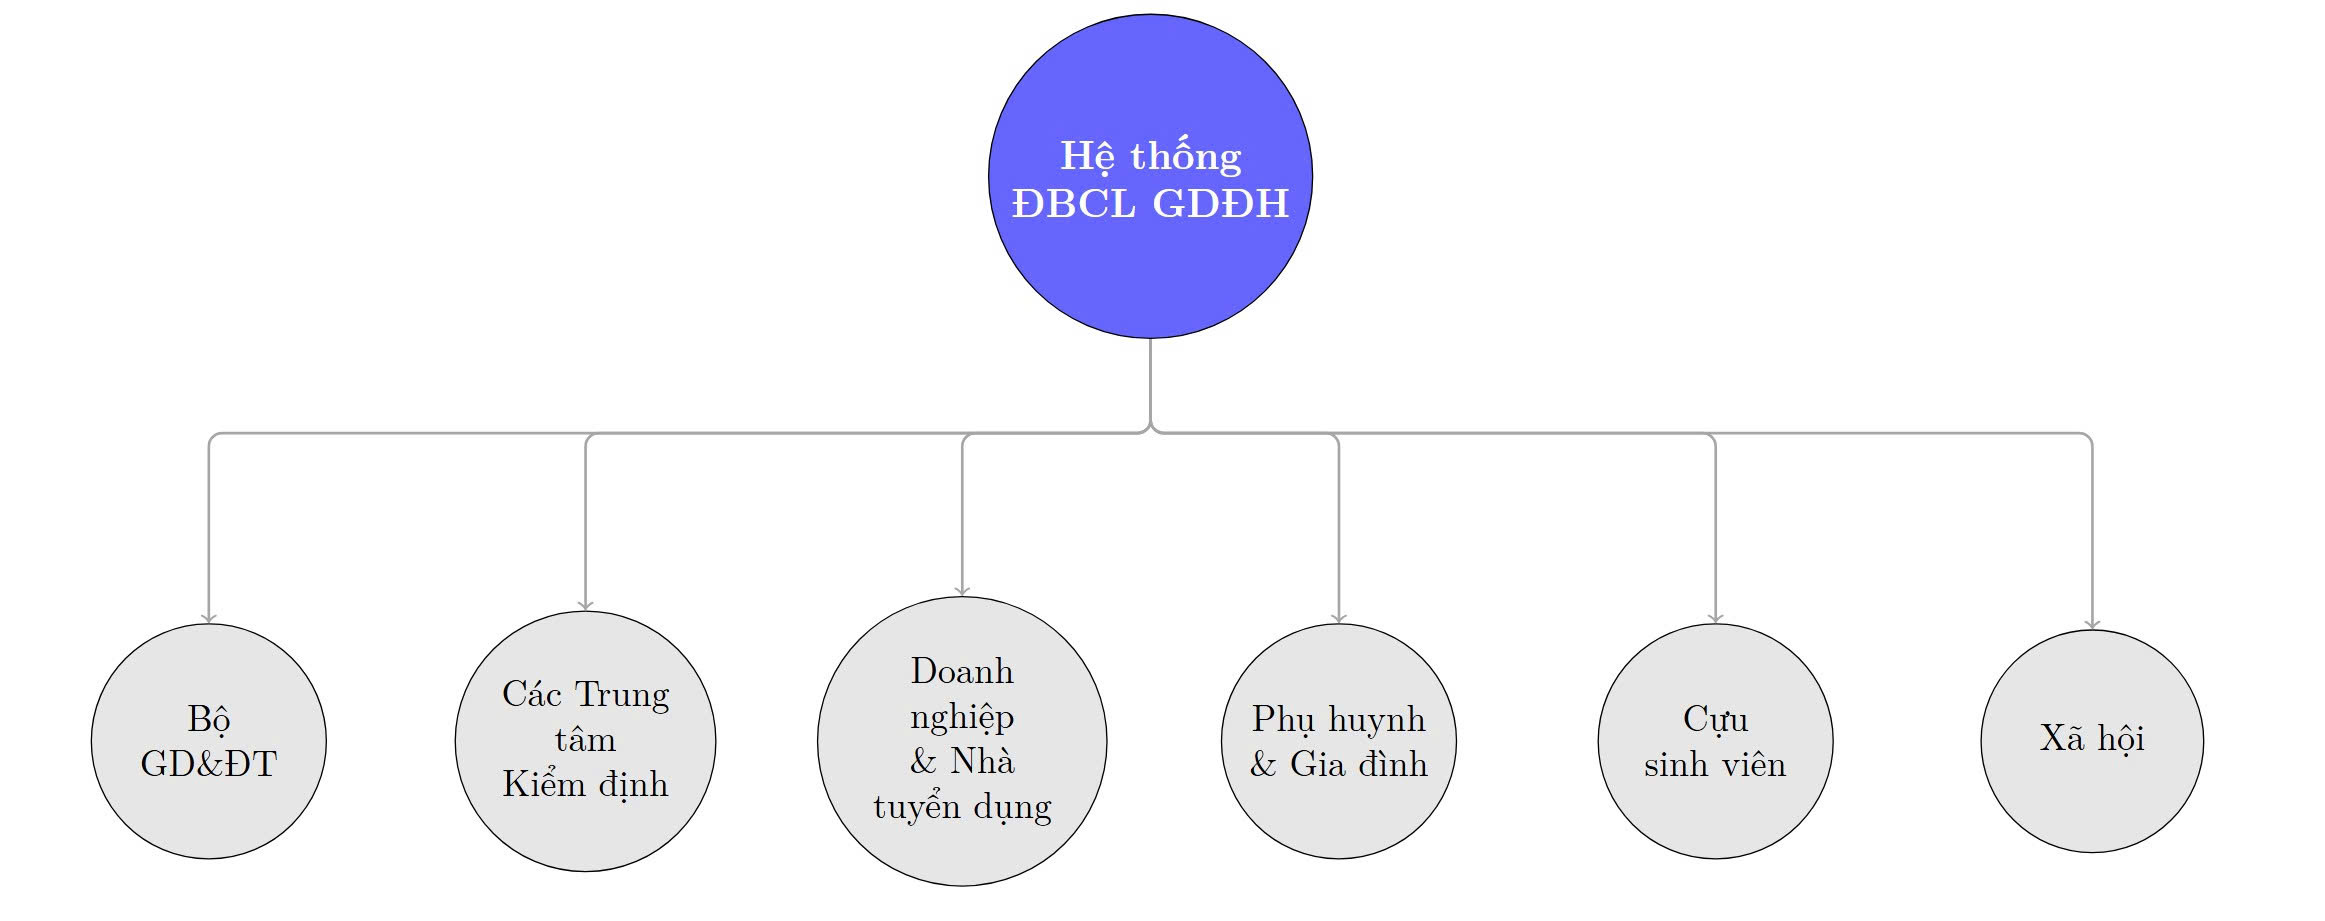
\includegraphics[width=\textwidth]{stakeholder_map.jpg} 
    \caption{Bản đồ các bên liên quan trong hệ thống ĐBCL GDĐH Việt Nam}
    \label{fig:stakeholder-map}
\end{figure}

\begin{itemize}
    \item \textbf{Các bên liên quan nội bộ (Internal Stakeholders):}
        \begin{itemize}
            \item \textit{Ban Lãnh đạo Trường (Hội đồng trường, Ban Giám hiệu):} Lợi ích chính là uy tín của nhà trường, sự ổn định tài chính, đạt được các chỉ số KPI, và tuân thủ quy định của cấp trên.
            \item \textit{Giảng viên và nhà nghiên cứu:} Lợi ích bao gồm tự do học thuật, điều kiện làm việc tốt, cơ hội phát triển chuyên môn, và giảm thiểu gánh nặng hành chính.
            \item \textit{Nhân viên hành chính (bao gồm cán bộ phòng ĐBCL):} Lợi ích là sự rõ ràng trong quy trình, có đủ nguồn lực để thực hiện công việc, và sự hợp tác từ các đơn vị khác.
            \item \textit{Sinh viên:} Lợi ích cốt lõi là chất lượng chương trình đào tạo, phương pháp giảng dạy hiệu quả, môi trường học tập tốt, cơ hội việc làm sau khi tốt nghiệp và mức học phí hợp lý.
        \end{itemize}
    \item \textbf{Các bên liên quan bên ngoài (External Stakeholders):}
        \begin{itemize}
            \item \textit{Bộ Giáo dục và Đào tạo:} Lợi ích là đảm bảo hệ thống GDĐH vận hành ổn định, có chất lượng đồng đều, đáp ứng các mục tiêu phát triển kinh tế-xã hội của quốc gia, và thực hiện trách nhiệm giải trình trước chính phủ và xã hội.
            \item \textit{Các Trung tâm Kiểm định Chất lượng Giáo dục:} Lợi ích là duy trì uy tín, sự chuyên nghiệp, và tính độc lập của tổ chức mình; hoàn thành nhiệm vụ kiểm định được giao.
            \item \textit{Doanh nghiệp và Nhà tuyển dụng:} Lợi ích là tuyển được nguồn nhân lực có kỹ năng và kiến thức phù hợp ngay với yêu cầu công việc, giảm chi phí đào tạo lại.
            \item \textit{Phụ huynh và Gia đình:} Lợi ích là sự đầu tư (thời gian, tiền bạc) cho con em mình mang lại kết quả xứng đáng (con có việc làm tốt, thành người).
            \item \textit{Cựu sinh viên:} Lợi ích là giá trị của tấm bằng và uy tín của trường cũ được nâng cao, tạo niềm tự hào và cơ hội trong mạng lưới nghề nghiệp.
            \item \textit{Xã hội:} Lợi ích là GDĐH góp phần tạo ra một xã hội công bằng, tiến bộ, có nguồn nhân lực chất lượng cao và duy trì các giá trị văn hóa.
        \end{itemize}
\end{itemize}
Bản đồ này cho thấy hệ thống ĐBCL phải phục vụ một mạng lưới lợi ích vô cùng đa dạng. Một quyết định cải tiến chất lượng, chẳng hạn như tăng cường yêu cầu thực hành cho sinh viên, có thể được doanh nghiệp hoan nghênh nhưng lại gặp phải sự phản đối từ giảng viên (do tăng khối lượng công việc) hoặc từ bộ phận tài chính (do tăng chi phí). Việc nhận diện và phân tích các mâu thuẫn lợi ích tiềm tàng này là bước đầu tiên để xây dựng một hệ thống ĐBCL hiệu quả.

% Kết thúc Gói 2
% ======================================================================
% TRANG 11-13: THUYẾT CÁC BÊN LIÊN QUAN (PHẦN 2)
% ======================================================================

\subsubsection{Sự ưu tiên của các bên liên quan (Stakeholder Salience)}

Việc nhận diện các bên liên quan chỉ là bước đầu tiên. Một thách thức lớn trong quản trị là làm thế nào để xử lý các yêu cầu đa dạng và thường xuyên mâu thuẫn từ các nhóm này. Không phải tất cả các bên liên quan đều có tầm ảnh hưởng như nhau. Mitchell, Agle, và Wood (1997) đã phát triển một mô hình có ảnh hưởng lớn để xác định "sự ưu tiên" (salience) của các bên liên quan, dựa trên ba thuộc tính cốt lõi \cite{Mitchell1997}:

\begin{enumerate}
    \item \textbf{Quyền lực (Power):} Khả năng của một bên liên quan trong việc áp đặt ý chí của mình lên tổ chức, buộc tổ chức phải làm những việc mà nếu không có áp lực đó, tổ chức sẽ không làm. Quyền lực có thể đến từ sự kiểm soát các nguồn lực quan trọng (như ngân sách), khả năng ban hành các quy định pháp lý, hoặc khả năng gây ảnh hưởng đến truyền thông.
    \item \textbf{Tính hợp pháp (Legitimacy):} Sự thừa nhận của xã hội rằng các yêu cầu hoặc hành động của một bên liên quan là chính đáng, phù hợp và đúng đắn trong một bối cảnh xã hội nhất định. Tính hợp pháp đến từ các quy định pháp luật, các hợp đồng, hoặc các chuẩn mực đạo đức xã hội.
    \item \textbf{Tính cấp thiết (Urgency):} Mức độ mà yêu cầu của một bên liên quan đòi hỏi sự chú ý ngay lập tức. Tính cấp thiết phụ thuộc vào hai yếu tố: sự nhạy cảm về thời gian (yêu cầu sẽ mất giá trị nếu không được xử lý kịp thời) và mức độ quan trọng của yêu cầu đó đối với bên liên quan.
\end{enumerate}

Dựa trên việc sở hữu một, hai, hoặc cả ba thuộc tính này, các bên liên quan có thể được phân thành các nhóm với mức độ ưu tiên khác nhau, từ nhóm "tiềm ẩn" (latent stakeholders, chỉ có 1 thuộc tính) đến nhóm "dứt khoát" (definitive stakeholders, có cả 3 thuộc tính) và cần được ban lãnh đạo quan tâm nhiều nhất.

Áp dụng mô hình này vào hệ thống ĐBCL GDĐH Việt Nam, chúng ta có thể lý giải một số hiện tượng quan trọng:
\begin{itemize}
    \item \textbf{Bộ Giáo dục và Đào tạo} là một bên liên quan "dứt khoát". Bộ có \textit{quyền lực} (thông qua việc phân bổ ngân sách, cấp phép), có \textit{tính hợp pháp} (theo Luật Giáo dục Đại học), và các yêu cầu của Bộ thường có \textit{tính cấp thiết} (gắn với các chu kỳ kiểm định, báo cáo). Do đó, tiếng nói của Bộ có trọng lượng lớn nhất và các trường đại học thường ưu tiên đáp ứng các yêu cầu này.
    \item \textbf{Doanh nghiệp/Nhà tuyển dụng} là một bên liên quan có \textit{tính hợp pháp} (họ có quyền đòi hỏi nguồn nhân lực chất lượng) và \textit{tính cấp thiết} (nhu cầu nhân lực thay đổi liên tục), nhưng lại thiếu \textit{quyền lực} trực tiếp để buộc các trường đại học phải thay đổi chương trình đào tạo ngay lập tức. Điều này giải thích tại sao, mặc dù các doanh nghiệp liên tục phàn nàn về chất lượng sinh viên, nhưng sự thay đổi trong chương trình đào tạo của các trường vẫn diễn ra chậm chạp.
    \item \textbf{Sinh viên và phụ huynh} có \textit{tính hợp pháp} và \textit{tính cấp thiết} cao, nhưng quyền lực của họ lại mang tính phân tán. Chỉ khi các yêu cầu của họ được tập hợp lại thông qua các cuộc khảo sát quy mô lớn hoặc qua các phương tiện truyền thông, quyền lực của họ mới trở nên rõ rệt hơn.
\end{itemize}
Như vậy, mô hình Salience giúp chúng ta hiểu rằng, quá trình ĐBCL không phải là một quá trình dân chủ tuyệt đối nơi mọi tiếng nói đều bình đẳng, mà là một "đấu trường chính trị" nơi các trường đại học phải liên tục cân nhắc và ưu tiên các yêu cầu từ những bên liên quan có ảnh hưởng lớn nhất.

\subsubsection{Ứng dụng và Phê phán Thuyết Các bên Liên quan}

Thuyết Các bên Liên quan cung cấp một công cụ phân tích hữu hiệu để giải mã các mâu thuẫn lợi ích trong hệ thống ĐBCL. Nó giúp trả lời câu hỏi: "Chất lượng cho ai?". Bằng cách xác định các bên liên quan và phân tích mức độ ưu tiên của họ, chúng ta có thể hiểu tại sao một số khía cạnh của chất lượng (ví dụ: số lượng bài báo quốc tế) lại được chú trọng hơn các khía cạnh khác (ví dụ: kỹ năng thực hành của sinh viên).

Tuy nhiên, thuyết này cũng có những giới hạn. Thách thức lớn nhất khi áp dụng nó là việc tìm ra một giải pháp tối ưu để \textbf{cân bằng} các lợi ích khi chúng đối kháng nhau. Ví dụ, việc tăng cường thực hành để đáp ứng yêu cầu của doanh nghiệp sẽ làm tăng chi phí đào tạo, có thể dẫn đến việc tăng học phí và gây ra sự phản đối từ sinh viên và phụ huynh. Thuyết Các bên Liên quan mô tả rất tốt cuộc tranh luận này nhưng không đưa ra một công thức rõ ràng để giải quyết nó. Hơn nữa, thuyết này tập trung vào các mối quan hệ và lợi ích hữu hình, nhưng ít chú ý đến các quy tắc và chuẩn mực văn hóa vô hình vốn có tác động mạnh mẽ đến hành vi của tổ chức – đây lại là điểm mạnh của Thuyết Tân Thể chế. Để hiểu các cơ chế trách nhiệm giải trình cụ thể, chúng ta cần đến một lý thuyết thứ ba.

\subsection{Thuyết Ủy nhiệm (Principal-Agent Theory)}
\label{subsec:uy_nhiem_nen_tang}

\subsubsection{Nguồn gốc và các khái niệm cốt lõi}
Thuyết Ủy nhiệm có nguồn gốc từ kinh tế học, đặc biệt là kinh tế học tài chính và lý thuyết về công ty, với các công trình nền tảng của các học giả như Stephen Ross, và đặc biệt là Michael Jensen và William Meckling vào những năm 1970 \cite{JensenMeckling1976}. Lý thuyết này được xây dựng để phân tích các vấn đề phát sinh trong các mối quan hệ mà ở đó một bên (bên ủy nhiệm - Principal) thuê hoặc giao phó cho một bên khác (bên nhận nhiệm - Agent) thực hiện một công việc nào đó thay mặt mình.

Vấn đề cốt lõi của mối quan hệ này (the agency problem) nảy sinh từ hai điều kiện cơ bản:
\begin{enumerate}
    \item \textbf{Xung đột mục tiêu (Conflict of Interest):} Lợi ích của bên ủy nhiệm và bên nhận nhiệm không phải lúc nào cũng đồng nhất. Ví dụ, cổ đông (principal) muốn tối đa hóa lợi nhuận, trong khi nhà quản lý (agent) có thể muốn tối đa hóa quyền lực hoặc các lợi ích cá nhân khác.
    \item \textbf{Bất đối xứng thông tin (Information Asymmetry):} Bên nhận nhiệm thường có nhiều thông tin hơn về công việc và nỗ lực của bản thân so với bên ủy nhiệm. Bên ủy nhiệm khó có thể giám sát một cách hoàn hảo mọi hành động của bên nhận nhiệm.
\end{enumerate}
Sự kết hợp của hai điều kiện này tạo ra hai loại rủi ro chính \cite{Eisenhardt1989}:
\begin{itemize}
    \item \textbf{Rủi ro đạo đức (Moral Hazard):} Sau khi hợp đồng đã được ký kết, bên nhận nhiệm có thể không nỗ lực hết mình vì bên ủy nhiệm không thể quan sát được mức độ nỗ lực của họ. Ví dụ, một trường đại học (agent) có thể không đầu tư tối đa vào việc cải tiến chất lượng giảng dạy sau khi đã nhận được ngân sách từ chính phủ (principal).
    \item \textbf{Lựa chọn đối nghịch (Adverse Selection):} Trước khi ký hợp đồng, bên nhận nhiệm có thể che giấu thông tin hoặc trình bày sai lệch về năng lực của mình để được chọn. Ví dụ, một trường đại học có thể "làm đẹp" báo cáo tự đánh giá để được một cơ quan kiểm định công nhận.
\end{itemize}
Để giải quyết các vấn đề này, lý thuyết đề xuất các giải pháp như thiết kế các hợp đồng hiệu quả, tạo ra các cơ chế khuyến khích (incentives) để dung hòa lợi ích, và quan trọng nhất là xây dựng các \textbf{hệ thống giám sát và báo cáo (monitoring and reporting systems)} để giảm thiểu sự bất đối xứng thông tin.

% Kết thúc Gói 3
% ======================================================================
% TRANG 16-18: THUYẾT ỦY NHIỆM (PHẦN 2) VÀ PHÊ PHÁN
% ======================================================================

\subsubsection{Hệ thống ĐBCL như một cơ chế giám sát và hợp đồng}

Từ lăng kính của Thuyết Ủy nhiệm, toàn bộ hệ thống ĐBCL bên ngoài có thể được xem như một cơ chế giám sát và hợp đồng phức tạp được thiết kế để giải quyết "vấn đề ủy nhiệm".

\paragraph{Mối quan hệ ủy nhiệm đa tầng:}
Trong GDĐH, mối quan hệ không chỉ đơn giản là giữa một Principal và một Agent. Nó là một chuỗi các mối quan hệ ủy nhiệm lồng vào nhau, tạo ra sự phức tạp trong việc quản lý và giám sát \cite{Borgos2013}. Ta có thể hình dung chuỗi quan hệ này tại Việt Nam như sau:
\begin{itemize}
    \item \textbf{Cấp 1 (Chính phủ $\rightarrow$ Bộ GD\&ĐT):} Chính phủ (Principal) giao cho Bộ GD\&ĐT (Agent) nhiệm vụ quản lý và phát triển hệ thống GDĐH quốc gia.
    \item \textbf{Cấp 2 (Bộ GD\&ĐT $\rightarrow$ Trường ĐH):} Bộ GD\&ĐT (Principal) cấp phép hoạt động và phân bổ ngân sách cho các trường ĐH (Agent), với kỳ vọng các trường sẽ đào tạo ra nguồn nhân lực chất lượng cao và thực hiện các nhiệm vụ nghiên cứu phục vụ xã hội.
    \item \textbf{Cấp 3 (Ban Giám hiệu $\rightarrow$ Khoa/Bộ môn):} Ban Giám hiệu (Principal) giao chỉ tiêu tuyển sinh và ngân sách cho các Khoa (Agent), yêu cầu các Khoa phải đảm bảo chất lượng đào tạo và nghiên cứu của đơn vị mình.
    \item \textbf{Cấp 4 (Khoa/Bộ môn $\rightarrow$ Giảng viên):} Trưởng khoa/bộ môn (Principal) phân công giảng dạy cho từng giảng viên (Agent) và kỳ vọng họ sẽ thực hiện bài giảng một cách tốt nhất.
\end{itemize}
Sự tồn tại của chuỗi ủy nhiệm này giải thích tại sao các yêu cầu từ cấp cao nhất (Chính phủ) thường bị "nhiễu" hoặc biến dạng khi đi xuống các cấp thấp hơn.

\paragraph{Các cơ chế giám sát trong thực tiễn ĐBCL:}
Để giảm thiểu rủi ro đạo đức và lựa chọn đối nghịch trong chuỗi quan hệ trên, các hệ thống ĐBCL đã phát triển nhiều cơ chế giám sát cụ thể:
\begin{itemize}
    \item \textbf{Hệ thống báo cáo (Reporting Systems):} Các yêu cầu về báo cáo tự đánh giá, báo cáo thường niên, thống kê số liệu... chính là công cụ để Principal ở cấp trên thu thập thông tin về hoạt động của Agent ở cấp dưới.
    \item \textbf{Kiểm định bên ngoài (External Accreditation):} Đây là một hình thức giám sát chuyên biệt và chính thức. Các cơ quan kiểm định (như VNU-CEA hay AUN-QA) đóng vai trò là "người kiểm toán" bên thứ ba, được Principal (Bộ GD\&ĐT) tin tưởng để xác minh thông tin và đánh giá hoạt động của các trường ĐH (Agent) \cite{Borgos2013}. Quá trình này giúp giảm đáng kể tình trạng bất đối xứng thông tin.
    \item \textbf{Hợp đồng dựa trên kết quả (Outcome-based Contracts):} Mặc dù chưa phổ biến ở Việt Nam, nhưng xu hướng trên thế giới là gắn việc phân bổ ngân sách với các kết quả đầu ra cụ thể (ví dụ: tỷ lệ sinh viên có việc làm, số lượng công bố quốc tế). Đây là một dạng hợp đồng được thiết kế để dung hòa lợi ích của Principal và Agent.
    \item \textbf{Xây dựng uy tín (Reputation Building):} Các hệ thống xếp hạng và công khai kết quả kiểm định cũng là một cơ chế giám sát. Uy tín của một trường (Agent) trở thành một tài sản quan trọng, và để bảo vệ tài sản đó, họ có động lực để hành động phù hợp với kỳ vọng của các Principal (sinh viên, xã hội).
\end{itemize}

\subsubsection{Ứng dụng và Phê phán Thuyết Ủy nhiệm}

Thuyết Ủy nhiệm cung cấp một bộ công cụ phân tích sắc bén để mổ xẻ cấu trúc trách nhiệm giải trình và các cơ chế giám sát trong hệ thống ĐBCL. Nó giải thích một cách logic tại sao lại cần có các quy trình báo cáo, thanh tra, kiểm định định kỳ. Đặc biệt, nó hữu ích trong việc phân tích các mối quan hệ mang tính hợp đồng, chẳng hạn như mối quan hệ giữa nhà nước và các trường đại học công lập được giao tự chủ.

Tuy nhiên, việc áp dụng một cách máy móc Thuyết Ủy nhiệm vào lĩnh vực GDĐH cũng có những giới hạn đáng kể \cite{RIHE2022}:
\begin{itemize}
    \item \textbf{Đơn giản hóa quá mức các mục tiêu:} Lý thuyết này giả định rằng mục tiêu của Principal có thể được định nghĩa rõ ràng. Nhưng trong GDĐH, "chất lượng" là một khái niệm đa chiều và khó đo lường. Mục tiêu của Chính phủ có thể là phát triển kinh tế, trong khi mục tiêu của xã hội là công bằng, và mục tiêu của cộng đồng học thuật là tự do sáng tạo. Ai mới là "Principal" thực sự?
    \item \textbf{Bỏ qua yếu tố văn hóa và chuẩn mực:} Thuyết này coi mối quan hệ giữa các chủ thể chủ yếu dựa trên lợi ích kinh tế và sự tính toán hợp lý. Nó không giải thích được vai trò của sự tin cậy, các giá trị chung, và các chuẩn mực nghề nghiệp (ví dụ: đạo đức nhà giáo) trong việc điều chỉnh hành vi của giảng viên và nhà trường.
    \item \textbf{Khó áp dụng các hợp đồng hoàn hảo:} Trong thực tế, rất khó để thiết kế một hợp đồng có thể lường hết mọi tình huống và đo lường chính xác mọi nỗ lực của Agent. "Sản phẩm" của giáo dục (con người) là vô cùng phức tạp và không thể được đo lường dễ dàng như sản phẩm công nghiệp.
\end{itemize}
Chính vì những giới hạn này, việc phân tích hệ thống ĐBCL không thể chỉ dựa vào Thuyết Ủy nhiệm. Cần phải kết hợp nó với Thuyết Tân Thể chế (để hiểu các quy tắc vô hình) và Thuyết Các bên Liên quan (để hiểu các lợi ích đa dạng) nhằm có được một bức tranh toàn cảnh và chính xác hơn.

% ======================================================================
% TRANG 19-20: CÁC MÔ HÌNH ĐBCL HIỆN ĐẠI
% ======================================================================
\section{Các Mô hình Đảm bảo Chất lượng Hiện đại trên Thế giới}
\label{sec:mo_hinh_hien_dai_the_gioi}

Sự phát triển của các lý thuyết về quản trị và những thách thức trong thực tiễn đã thúc đẩy sự ra đời của các mô hình ĐBCL ngày càng tinh vi hơn. Các mô hình này không còn bám cứng vào một lý thuyết duy nhất mà là sự tổng hợp và nỗ lực vượt lên trên các giới hạn của các cách tiếp cận truyền thống. Trong đó, hai xu hướng nổi bật, có ý nghĩa tham khảo quan trọng cho Việt Nam, là Mô hình Lai ghép và Khung Thích ứng \cite{HybridModel2023, AdaptiveQA2022}.

\subsection{Mô hình Lai ghép (Hybrid Model): Dung hòa Trách nhiệm Giải trình và Cải tiến}

\subsubsection{Bối cảnh Ra đời và Triết lý}
Các hệ thống ĐBCL truyền thống thường rơi vào một trong hai thái cực. Một là, hệ thống quá chú trọng vào \textbf{trách nhiệm giải trình (accountability)} đối với bên ngoài (top-down), dẫn đến việc các trường chỉ tập trung vào việc tuân thủ quy định một cách hình thức, đối phó, tạo ra một "văn hóa tuân thủ" (culture of compliance) thay vì cải tiến thực chất. Đây là mô hình gần với tư duy của Thuyết Ủy nhiệm. Hai là, hệ thống quá chú trọng vào \textbf{cải tiến nội tại (improvement)} (bottom-up), trao toàn quyền cho các đơn vị tự đánh giá, dẫn đến việc thiếu các tiêu chuẩn chung và khó đảm bảo trách nhiệm giải trình với xã hội.

Mô hình Lai ghép ra đời như một nỗ lực để giải quyết sự căng thẳng này \cite{EUA_Integration}. Triết lý của nó là công nhận và tích hợp cả hai mục tiêu. Nó cho rằng một hệ thống ĐBCL bền vững phải vừa đáp ứng được các yêu cầu kiểm soát và minh bạch từ bên ngoài, vừa phải khơi dậy được động lực cải tiến và phát triển văn hóa chất lượng từ bên trong. Thay vì xem accountability và improvement là hai mục tiêu đối lập, mô hình lai ghép coi chúng là hai mặt của một đồng xu, bổ trợ và củng cố lẫn nhau. Ví dụ, các yêu cầu giải trình minh bạch từ bên ngoài có thể cung cấp dữ liệu và áp lực cần thiết để thúc đẩy các nỗ lực cải tiến bên trong. Ngược lại, một văn hóa cải tiến mạnh mẽ từ bên trong sẽ giúp nhà trường dễ dàng đáp ứng và vượt qua các yêu cầu giải trình từ bên ngoài.

\subsubsection{Các Thành phần và Đặc điểm}
Một mô hình lai ghép điển hình thường có các đặc điểm sau:
\begin{itemize}
    \item \textbf{Khung tiêu chuẩn kép:} Hệ thống có thể bao gồm một bộ tiêu chuẩn tối thiểu (minimum standards) bắt buộc cho mục đích giải trình, và một bộ tiêu chuẩn nâng cao (enhancement standards) mang tính khuyến khích cho mục đích cải tiến.
    \item \textbf{Quy trình lồng ghép:} Các hoạt động kiểm định bên ngoài được thiết kế để không chỉ kiểm tra sự tuân thủ, mà còn đưa ra các khuyến nghị mang tính xây dựng, hỗ trợ quá trình cải tiến của nhà trường. Ngược lại, kết quả từ các hoạt động tự đánh giá và cải tiến nội bộ được sử dụng làm bằng chứng quan trọng trong các đợt kiểm định bên ngoài.
    \item \textbf{Vai trò linh hoạt của cơ quan ĐBCL:} Các cơ quan ĐBCL bên ngoài không chỉ đóng vai trò là "người phán xét" mà còn là "người bạn đồng hành", "nhà tư vấn", hỗ trợ các trường trong quá trình cải tiến.
\end{itemize}
Kinh nghiệm của các hệ thống ĐBCL tại Châu Âu, đặc biệt là sau Tiến trình Bologna, cho thấy một xu hướng rõ rệt trong việc dịch chuyển sang các mô hình lai ghép, nơi các quy trình kiểm định ngày càng được thiết kế để phục vụ cho mục tiêu nâng cao chất lượng (enhancement-led accreditation) \cite{EUA_Integration}. Thực tiễn tại Việt Nam, với việc vừa phải đáp ứng các tiêu chuẩn quốc gia của Bộ GD\&ĐT, vừa tham gia các chương trình kiểm định khu vực như AUN-QA, cũng đang cho thấy những dấu hiệu của một mô hình lai ghép đang dần hình thành, dù có thể chưa hoàn toàn tự giác \cite{VNU-CEA2023, HangNguyen2017}.

% Kết thúc Gói 4
% ======================================================================
% TRANG 21-22: KHUNG THÍCH ỨNG
% ======================================================================

\subsection{Khung Thích ứng (Adaptive Framework): Quản lý Chất lượng trong một Thế giới Biến đổi}
\label{subsec:khung_thich_ung}

\subsubsection{So sánh với các phương pháp truyền thống}
Nếu Mô hình Lai ghép giải quyết mâu thuẫn về \textit{mục tiêu} của ĐBCL, thì Khung Thích ứng giải quyết vấn đề về \textit{quy trình} triển khai trong một môi trường không ổn định và phức tạp. Phương pháp quản lý dự án truyền thống, thường được biết đến với tên gọi mô hình "thác nước" (Waterfall Model), hoạt động theo một trình tự tuyến tính nghiêm ngặt: Lập kế hoạch $\rightarrow$ Thiết kế $\rightarrow$ Thực hiện $\rightarrow$ Kiểm tra $\rightarrow$ Bàn giao. Mô hình này giả định rằng tất cả các yêu cầu và điều kiện đều có thể được xác định rõ ràng ngay từ đầu, và môi trường sẽ không thay đổi trong suốt quá trình.

Tuy nhiên, thực tế trong GDĐH, đặc biệt tại Việt Nam, lại hoàn toàn khác. Các chính sách của Bộ có thể thay đổi, nhu cầu của thị trường lao động biến động, công nghệ giáo dục phát triển nhanh chóng, và nguồn lực của nhà trường cũng không ổn định. Việc áp dụng một kế hoạch ĐBCL cứng nhắc, kéo dài 5 năm theo mô hình thác nước thường dẫn đến tình trạng kế hoạch trở nên lỗi thời ngay khi chưa thực hiện xong.

Khung Thích ứng (Adaptive Framework), vốn có nguồn gốc từ lĩnh vực phát triển phần mềm linh hoạt (Agile), ra đời để giải quyết chính những vấn đề này \cite{Wysocki2009}. Thay vì cố gắng lập một kế hoạch hoàn hảo từ đầu, phương pháp này chia nhỏ dự án thành các chu kỳ ngắn, lặp đi lặp lại. Cuối mỗi chu kỳ, nhóm dự án sẽ đánh giá lại kết quả, thu thập phản hồi và điều chỉnh kế hoạch cho chu kỳ tiếp theo.

\subsubsection{Các Nguyên tắc Cốt lõi của Khung Thích ứng}
Một khung ĐBCL mang tính thích ứng sẽ vận hành dựa trên các nguyên tắc sau:
\begin{itemize}
    \item \textbf{Học hỏi lặp lại (Iterative Learning):} Toàn bộ quy trình ĐBCL được xem là một quá trình học hỏi. Thay vì một chu kỳ đánh giá lớn 5 năm một lần, nhà trường có thể thực hiện các chu kỳ đánh giá nhỏ hơn (ví dụ: hàng năm) cho từng khía cạnh cụ thể (như phương pháp giảng dạy, dịch vụ sinh viên). Kết quả của mỗi chu kỳ sẽ cung cấp thông tin để cải tiến chu kỳ sau.
    \item \textbf{Vòng lặp phản hồi (Feedback Loops):} Khung này tạo ra các vòng lặp phản hồi nhanh chóng và thường xuyên. Thay vì chờ đến cuối chu kỳ 5 năm mới có báo cáo kiểm định, nhà trường có thể tổ chức các buổi họp phản hồi với sinh viên, giảng viên, và doanh nghiệp sau mỗi học kỳ hoặc mỗi năm học.
    \item \textbf{Phát triển tăng dần (Incremental Development):} Các cải tiến về chất lượng không cần phải được thực hiện đồng loạt, mà có thể được triển khai dần dần, theo từng phần. Ví dụ, trong năm đầu tiên, nhà trường có thể tập trung cải tiến hệ thống lấy ý kiến sinh viên; năm thứ hai, tập trung vào việc đổi mới phương pháp đánh giá kết quả học tập.
    \item \textbf{Sự ưu tiên dựa trên giá trị (Value-driven Prioritization):} Ở mỗi chu kỳ, các hoạt động cải tiến sẽ được ưu tiên dựa trên giá trị mà chúng mang lại cho các bên liên quan quan trọng nhất tại thời điểm đó.
\end{itemize}

\subsubsection{Tính phù hợp với bối cảnh Việt Nam}
Lập luận cho rằng Khung Thích ứng đặc biệt phù hợp với bối cảnh Việt Nam dựa trên các lý do sau:
\begin{itemize}
    \item \textbf{Môi trường chính sách năng động:} Các quy định và chính sách về GDĐH ở Việt Nam có thể thay đổi nhanh chóng. Một khung thích ứng cho phép các trường linh hoạt điều chỉnh chiến lược ĐBCL của mình để phù hợp với các yêu cầu mới mà không cần phải phá bỏ toàn bộ kế hoạch cũ.
    \item \textbf{Hạn chế về nguồn lực:} Thay vì cần một khoản đầu tư lớn để cải cách toàn diện, các trường có thể thực hiện các cải tiến nhỏ, tăng dần, phù hợp với nguồn lực hạn hẹp của mình trong từng giai đoạn.
    \item \textbf{Xây dựng năng lực từ từ:} Việc áp dụng một hệ thống ĐBCL phức tạp ngay lập tức có thể gây quá tải cho đội ngũ nhân sự. Khung thích ứng cho phép nhà trường vừa làm vừa học, xây dựng năng lực ĐBCL một cách từ từ và bền vững.
\end{itemize}
Như vậy, sự kết hợp giữa triết lý của Mô hình Lai ghép và quy trình của Khung Thích ứng sẽ tạo ra một phương pháp tiếp cận ĐBCL vừa toàn diện về mục tiêu, vừa linh hoạt và thực tế về cách thức triển khai. Đây chính là nền tảng để xây dựng mô hình đề xuất cho Việt Nam.

% ======================================================================
% TRANG 23-25: ĐỀ XUẤT MÔ HÌNH V-AQA
% ======================================================================
\section{Đề xuất Mô hình Phân tích cho GDĐH Việt Nam: Mô hình Lai ghép và Thích ứng (V-AQA)}
\label{sec:mo_hinh_V-AQA_de_xuat}

\subsection{Luận giải cho sự cần thiết của một mô hình tích hợp}
\label{subsec:luan_giai_V-AQA}
Qua phân tích ở các phần trên, có thể thấy rằng việc sử dụng một lý thuyết đơn lẻ để phân tích hệ thống ĐBCL GDĐH Việt Nam sẽ không đầy đủ và có thể dẫn đến những kết luận phiến diện.
\begin{itemize}
    \item \textbf{Nếu chỉ dùng Thuyết Tân Thể chế}, chúng ta sẽ giải thích được tại sao các trường lại tuân thủ các quy định một cách hình thức, nhưng khó lý giải được những nỗ lực cải tiến thực chất từ bên trong hay các mâu thuẫn lợi ích.
    \item \textbf{Nếu chỉ dùng Thuyết Các bên Liên quan}, chúng ta sẽ thấy được bức tranh đa dạng về lợi ích, nhưng lại thiếu công cụ để phân tích tại sao tiếng nói của một số bên lại có trọng lượng hơn những bên khác, và cũng không giải thích được các cơ chế báo cáo, giám sát.
    \item \textbf{Nếu chỉ dùng Thuyết Ủy nhiệm}, chúng ta sẽ hiểu rõ về cấu trúc trách nhiệm giải trình, nhưng lại bỏ qua các yếu tố văn hóa, chuẩn mực và các mối quan hệ hợp tác phức tạp không thể quy về một hợp đồng đơn thuần.
\end{itemize}

Do đó, bối cảnh Việt Nam đòi hỏi một khung phân tích tích hợp, một mô hình có khả năng dung hợp các góc nhìn khác nhau. Luận án này đề xuất một mô hình như vậy, với tên gọi \textbf{Mô hình Đảm bảo Chất lượng Lai ghép và Thích ứng cho Giáo dục Đại học Việt Nam (The Vietnam - Adaptive Quality Assurance Model, viết tắt là V-AQA)}.

Mô hình này mang tính \textbf{lai ghép (Hybrid)} vì nó công nhận và tìm cách dung hòa hai mục tiêu song song và đôi khi mâu thuẫn:
\begin{enumerate}
    \item \textbf{Trách nhiệm giải trình với bên ngoài (External Accountability):} Đáp ứng các yêu cầu từ Bộ GD\&ĐT, các cơ quan kiểm định, và xã hội để có được tính hợp pháp và nguồn lực (phản ánh góc nhìn của Thuyết Tân Thể chế và Thuyết Ủy nhiệm).
    \item \textbf{Cải tiến từ bên trong (Internal Improvement):} Tạo ra giá trị cho các bên liên quan nội bộ (sinh viên, giảng viên) và thúc đẩy một văn hóa chất lượng tự thân (phản ánh góc nhìn của Thuyết Các bên Liên quan).
\end{enumerate}

Đồng thời, mô hình này mang tính \textbf{thích ứng (Adaptive)} vì nó đề cao sự linh hoạt trong quá trình triển khai, cho phép các trường đại học điều chỉnh các hoạt động ĐBCL của mình theo từng chu kỳ ngắn, dựa trên phản hồi và sự thay đổi của môi trường, thay vì tuân theo một kế hoạch 5 năm cứng nhắc.

\subsection{Cấu trúc Mô hình V-AQA và các thành tố cốt lõi}
\label{subsec:cau_truc_V-AQA}

Mô hình V-AQA được cấu trúc như một ngôi đền, với nền móng là các lý thuyết, mái nhà là mục tiêu cuối cùng, và được chống đỡ bởi năm trụ cột là năm thành tố cốt lõi. Năm thành tố này không hoạt động độc lập mà tương tác và củng cố lẫn nhau để tạo nên một hệ thống vững chắc (Xem Hình \ref{fig:v-aqa-model-detailed}).

\begin{figure}[h!]
    \centering
    \begin{tikzpicture}[
        base/.style={rectangle, rounded corners, minimum width=10cm, minimum height=1.5cm, text centered, draw=black, fill=gray!20, text width=9cm, font=\small},
        pillar/.style={rectangle, minimum width=2.2cm, minimum height=4cm, text centered, text width=2cm, draw=black, fill=blue!20, font=\small\bfseries, drop shadow},
        % Style cho khối mái nhà
        roof/.style={trapezium, trapezium left angle=70, trapezium right angle=110, 
            minimum width=8cm, 
            minimum height=1.2cm, % Chiều cao tối thiểu
            text centered, text width=8cm, % Độ rộng văn bản
            draw=black, fill=green!30, font=\bfseries, 
            drop shadow
        }
    ]
        % Vẽ nền móng (Các lý thuyết nền)
        \node (base) [base] {
            \textbf{Nền tảng lý thuyết:} Thuyết Tân Thể chế, Thuyết Các bên Liên quan, Thuyết Ủy nhiệm
        };

        % Vẽ 5 trụ cột
        \node (p1) [pillar, above=1cm of base.west, xshift=1.2cm] {1. Lãnh đạo \& Quản trị};
        \node (p2) [pillar, right=0.5cm of p1] {2. Văn hóa Chất lượng};
        \node (p3) [pillar, right=0.5cm of p2] {3. Sự tham gia của các Bên liên quan};
        \node (p4) [pillar, right=0.5cm of p3] {4. Quy trình Nội bộ};
        \node (p5) [pillar, right=0.5cm of p4] {5. Hợp tác \& Phối hợp};
        
        % Vẽ mái nhà (Mục tiêu cuối cùng)
        \node (roof) [roof, above=0.5cm of p3] {Đảm bảo và Nâng cao Chất lượng GDĐH Bền vững};

    \end{tikzpicture}
    \caption{Mô hình Đảm bảo Chất lượng Lai ghép và Thích ứng (V-AQA)}
    \label{fig:v-aqa-model-detailed}
\end{figure}

\subsubsection{Phân tích chi tiết Thành tố 1: Lãnh đạo \& Quản trị (Leadership \& Governance)}
\label{subsubsec:thanh_to_1}

\paragraph{Định nghĩa và Phạm vi:}
Thành tố Lãnh đạo \& Quản trị là yếu tố khởi nguồn, định hướng và cung cấp nguồn lực cho toàn bộ hệ thống ĐBCL. Nó không chỉ đơn thuần là các hoạt động quản lý hành chính, mà còn là khả năng của ban lãnh đạo trong việc xây dựng tầm nhìn, truyền cảm hứng, và thiết lập một cơ cấu quản trị hiệu quả để hiện thực hóa tầm nhìn đó. Trong bối cảnh Việt Nam, thành tố này bao gồm vai trò của Hội đồng trường, Ban Giám hiệu, và lãnh đạo các cấp khoa, phòng ban. Nó thể hiện qua việc ban hành các chiến lược, chính sách về chất lượng và sự cam kết thực hiện chúng.

\paragraph{Cơ sở Lý thuyết và Thực tiễn:}
Thành tố này được soi chiếu mạnh mẽ bởi \textbf{Thuyết Ủy nhiệm} và \textbf{Thuyết Tân Thể chế}.
\begin{itemize}
    \item Dưới góc độ Thuyết Ủy nhiệm, ban lãnh đạo nhà trường vừa là \textit{Agent} của cơ quan quản lý cấp trên (Bộ GD\&ĐT), có trách nhiệm thực thi các chính sách quốc gia; vừa là \textit{Principal} đối với các đơn vị cấp dưới (khoa, bộ môn), có trách nhiệm giám sát và đảm bảo các đơn vị này hoạt động hiệu quả. Sự rõ ràng trong cơ cấu quản trị và phân định trách nhiệm là điều kiện tiên quyết để giải quyết các vấn đề ủy nhiệm nội bộ.
    \item Dưới góc độ Thuyết Tân Thể chế, lãnh đạo là người "đọc" và diễn giải các áp lực từ trường thể chế. Họ là người quyết định chiến lược của nhà trường: sẽ tuân thủ một cách thụ động, bắt chước các mô hình thành công, hay chủ động tìm kiếm một con đường riêng để tạo ra sự khác biệt và tính hợp pháp độc đáo. Tầm nhìn của lãnh đạo sẽ định hình cách nhà trường tương tác với môi trường bên ngoài.
\end{itemize}

\paragraph{Các Chỉ báo và Biểu hiện trong Thực tiễn:}
Để đánh giá mức độ phát triển của thành tố này tại một trường đại học, có thể xem xét các chỉ báo sau:
\begin{itemize}
    \item Sự tồn tại và mức độ chi tiết của một \textit{chiến lược chất lượng} cấp trường, được tích hợp vào chiến lược phát triển chung của nhà trường.
    \item Tần suất và nội dung các cuộc họp của Ban Giám hiệu, Hội đồng trường có liên quan đến vấn đề ĐBCL.
    \item Mức độ phân bổ nguồn lực (tài chính, nhân sự) cho các hoạt động ĐBCL.
    \item Sự rõ ràng trong văn bản quy định chức năng, nhiệm vụ của các đơn vị liên quan đến ĐBCL.
    \item Kết quả khảo sát ý kiến của cán bộ, giảng viên về sự cam kết và vai trò định hướng của ban lãnh đạo đối với công tác chất lượng.
\end{itemize}
Việc phân tích các chỉ báo này sẽ được thực hiện chi tiết trong chương thực trạng của luận án.

% Kết thúc Gói 5
% ======================================================================
% TRANG 26-28: PHÂN TÍCH CHI TIẾT THÀNH TỐ 2: VĂN HÓA CHẤT LƯỢNG
% ======================================================================

\subsubsection{Phân tích chi tiết Thành tố 2: Văn hóa Chất lượng (Quality Culture)}
\label{subsubsec:thanh_to_2}

\paragraph{Định nghĩa và Phạm vi:}
Văn hóa chất lượng không chỉ đơn thuần là sự nhận thức hay các khẩu hiệu về chất lượng, mà là một tập hợp các giá trị, niềm tin, kỳ vọng và cam kết được chia sẻ, định hình hành vi của mọi thành viên trong một cơ sở giáo dục đối với việc đảm bảo và nâng cao chất lượng \cite{HarveyStensaker}. Nó là "cách chúng ta làm việc ở đây" (the way we do things around here) khi nói về chất lượng. Thành tố này đối lập với một "văn hóa tuân thủ" (culture of compliance), nơi các hoạt động ĐBCL chỉ được thực hiện một cách máy móc để đáp ứng các yêu cầu từ bên ngoài.

Phạm vi của văn hóa chất lượng rất rộng, nó thấm sâu vào mọi ngóc ngách của đời sống học thuật, từ cách một giảng viên chuẩn bị bài giảng, cách một khoa tổ chức các buổi hội thảo chuyên môn, cho đến cách ban lãnh đạo nhà trường đưa ra các quyết định chiến lược. Một văn hóa chất lượng mạnh mẽ sẽ biến ĐBCL từ một gánh nặng hành chính thành một động lực nội tại cho sự phát triển của cá nhân và tổ chức.

\paragraph{Cơ sở Lý thuyết và các Chiều kích của Văn hóa Chất lượng:}
Văn hóa chất lượng được soi chiếu rõ nét nhất qua lăng kính của \textbf{Thuyết Tân Thể chế}, đặc biệt là hai trụ cột \textit{chuẩn tắc (normative)} và \textit{văn hóa-nhận thức (cultural-cognitive)}.
\begin{itemize}
    \item \textbf{Khía cạnh chuẩn tắc:} Văn hóa chất lượng được hình thành và củng cố thông qua các chuẩn mực nghề nghiệp. Khi "cải tiến liên tục" hay "lấy người học làm trung tâm" trở thành một chuẩn mực được cộng đồng học thuật coi trọng, các cá nhân sẽ có xu hướng hành động theo chuẩn mực đó để được xem là một nhà giáo, nhà quản lý chuyên nghiệp.
    \item \textbf{Khía cạnh văn hóa-nhận thức:} Văn hóa chất lượng tồn tại như một kịch bản, một lẽ thường được chấp nhận mà không cần suy nghĩ. Khi đó, việc thu thập phản hồi từ sinh viên hay việc rà soát chương trình đào tạo định kỳ không còn là một yêu cầu, mà là một hành động "hiển nhiên" phải làm.
\end{itemize}

Để phân tích văn hóa chất lượng một cách hệ thống, có thể sử dụng mô hình của Harvey và Stensaker (2008), phân loại văn hóa chất lượng thành bốn dạng, phản ánh mức độ trưởng thành của tổ chức \cite{HarveyStensaker}:
\begin{enumerate}
    \item \textbf{Văn hóa Phản ứng (Reactive Culture):} Tổ chức chỉ quan tâm đến chất lượng khi có vấn đề xảy ra hoặc khi có yêu cầu kiểm tra từ bên ngoài. Đây là cấp độ thấp nhất.
    \item \textbf{Văn hóa Đáp ứng (Responsive Culture):} Tổ chức bắt đầu xây dựng các quy trình và hệ thống để đáp ứng các yêu cầu về chất lượng, nhưng động lực vẫn chủ yếu đến từ bên ngoài. Nhiều trường đại học Việt Nam hiện đang ở giai đoạn này, xây dựng các phòng ĐBCL và quy trình để phục vụ các đợt kiểm định.
    \item \textbf{Văn hóa Tái tạo/Cải tiến (Regenerative Culture):} Đây là một bước nhảy vọt. Tổ chức có khả năng tự đánh giá, tự tìm ra các vấn đề và chủ động thực hiện các chu trình cải tiến liên tục. Động lực cải tiến đến từ bên trong.
    \item \textbf{Văn hóa Sinh sản/Lan tỏa (Reproductive Culture):} Ở cấp độ cao nhất, tổ chức không chỉ tự cải tiến mà còn trở thành hình mẫu, lan tỏa các thực hành tốt nhất về chất lượng ra bên ngoài, định hình các chuẩn mực cho các tổ chức khác.
\end{enumerate}
Mô hình này cung cấp một công cụ hữu ích để chẩn đoán và xác định mục tiêu phát triển văn hóa chất lượng cho một trường đại học.

\paragraph{Các Chỉ báo và Biểu hiện trong Thực tiễn Việt Nam:}
Văn hóa chất lượng là một khái niệm trừu tượng, nhưng có thể được đo lường gián tiếp thông qua các chỉ báo và biểu hiện cụ thể:
\begin{itemize}
    \item \textbf{Sự cam kết của lãnh đạo:} Các phát biểu công khai, các văn bản chiến lược, và việc phân bổ nguồn lực cho thấy ĐBCL có phải là ưu tiên thực sự hay không.
    \item \textbf{Thái độ của giảng viên và nhân viên:} Kết quả từ các cuộc khảo sát về sự hài lòng trong công việc, thái độ đối với các hoạt động ĐBCL (xem đó là gánh nặng hay cơ hội), và mức độ tham gia tự nguyện vào các hoạt động cải tiến.
    \item \textbf{Ngôn ngữ sử dụng trong nội bộ:} Các văn bản và các cuộc họp nội bộ sử dụng ngôn ngữ "tuân thủ", "đáp ứng yêu cầu" hay ngôn ngữ "nâng cao", "cải tiến", "xuất sắc"?
    \item \textbf{Cơ chế công nhận và khen thưởng:} Nhà trường có các cơ chế để vinh danh và khen thưởng các cá nhân, đơn vị có sáng kiến cải tiến chất lượng hay không?
\end{itemize}
Thực trạng tại Việt Nam, như được phản ánh qua các báo cáo chuyên gia, cho thấy nhiều trường đại học vẫn đang vật lộn để chuyển từ văn hóa "đáp ứng" sang văn hóa "cải tiến". Áp lực từ các đợt kiểm định thường tạo ra các hoạt động mang tính thời vụ, và văn hóa chất lượng chưa thực sự thấm sâu vào hoạt động hàng ngày của mỗi giảng viên \cite{ExpertPerspectivesVN, CommonFailureCriteria}. Đây là một trong những thách thức lớn nhất mà mô hình V-AQA cần phải giải quyết.

% ======================================================================
% TRANG 29-30: PHÂN TÍCH CHI TIẾT THÀNH TỐ 3: SỰ THAM GIA CỦA CÁC BÊN LIÊN QUAN
% ======================================================================

\subsubsection{Phân tích chi tiết Thành tố 3: Sự tham gia của các Bên liên quan (Stakeholder Engagement)}
\label{subsubsec:thanh_to_3}

\paragraph{Định nghĩa và Phạm vi:}
Sự tham gia của các bên liên quan không chỉ đơn thuần là việc "khảo sát ý kiến" hay "tổ chức hội thảo". Nó là một quá trình có hệ thống, có chủ đích nhằm thu hút các bên liên quan vào các chu trình ĐBCL, từ việc thiết kế chương trình đào tạo, đến quá trình giảng dạy và học tập, đánh giá và cải tiến. Đây là sự hiện thực hóa của triết lý "chất lượng cho ai?", công nhận rằng một chương trình đào tạo chất lượng phải tạo ra giá trị cho nhiều nhóm đối tượng khác nhau.

Phạm vi của sự tham gia rất rộng, bao gồm nhiều hình thức khác nhau, từ mức độ thấp đến cao:
\begin{itemize}
    \item \textbf{Thông tin (Informing):} Cung cấp thông tin một chiều cho các bên liên quan.
    \item \textbf{Tham vấn (Consulting):} Lấy ý kiến, phản hồi từ các bên liên quan.
    \item \textbf{Tham gia (Involving):} Làm việc trực tiếp với các bên liên quan trong suốt quá trình.
    \item \textbf{Hợp tác (Collaborating):} Trở thành đối tác trong việc ra quyết định.
    \item \textbf{Trao quyền (Empowering):} Trao quyền ra quyết định cuối cùng cho các bên liên quan.
\end{itemize}
Một hệ thống ĐBCL trưởng thành cần có các cơ chế cho các mức độ tham gia khác nhau, tùy thuộc vào từng vấn đề và từng bên liên quan cụ thể \cite{Arnstein1969}.

\paragraph{Cơ sở Lý thuyết và Thực tiễn:}
Thành tố này là sự vận dụng trực tiếp của \textbf{Thuyết Các bên Liên quan}. Nó chuyển trọng tâm từ một mô hình quản trị khép kín, hướng nội sang một mô hình mở, hướng ngoại. Đây cũng là một thành tố cốt lõi của Mô hình Lai ghép, vì chính những phản hồi và yêu cầu từ các bên liên quan bên ngoài là động lực quan trọng cho các hoạt động cải tiến bên trong.

Thực tiễn quốc tế, đặc biệt là kinh nghiệm từ Châu Âu, cho thấy sự tham gia của các bên liên quan, đặc biệt là sinh viên và nhà tuyển dụng, là một yếu tố không thể thiếu trong các hệ thống ĐBCL hiện đại. Các bộ tiêu chuẩn như AUN-QA cũng đặt ra các yêu cầu rất rõ ràng về việc thu thập và sử dụng ý kiến phản hồi từ các bên liên quan trong việc rà soát và cải tiến chương trình đào tạo \cite{ENQA_Stakeholder2018, AUN-QAGuide}.

\paragraph{Các Chỉ báo và Biểu hiện trong Thực tiễn Việt Nam:}
Mức độ phát triển của thành tố này có thể được đánh giá qua các chỉ báo:
\begin{itemize}
    \item \textbf{Sự tồn tại của các hội đồng có sự tham gia của bên ngoài:} Ví dụ, Hội đồng Khoa học và Đào tạo, Hội đồng tư vấn doanh nghiệp (Industry Advisory Board) cho từng chương trình.
    \item \textbf{Tần suất và tính thực chất của các hoạt động tham vấn:} Số lượng các cuộc hội thảo với nhà tuyển dụng, khảo sát cựu sinh viên, các kênh phản hồi dành cho sinh viên.
    \item \textbf{Minh chứng về sự tác động:} Có bằng chứng cụ thể cho thấy các chương trình đào tạo đã được điều chỉnh, cập nhật dựa trên phản hồi từ doanh nghiệp hoặc cựu sinh viên hay không.
    \item \textbf{Vai trò của sinh viên trong các hội đồng:} Sinh viên có đại diện trong các hội đồng cấp khoa, cấp trường hay không, và tiếng nói của họ có được lắng nghe và ghi nhận một cách thực chất hay không.
\end{itemize}
Tại Việt Nam, đây là một trong những thành tố còn nhiều hạn chế. Các báo cáo thường chỉ ra rằng liên kết giữa nhà trường và doanh nghiệp còn lỏng lẻo và mang tính hình thức. Các chương trình đào tạo thường được xây dựng chủ yếu dựa trên quan điểm của đội ngũ học thuật mà ít có sự tham gia thực chất của các nhà tuyển dụng \cite{CommonFailureCriteria}. Do đó, việc tăng cường sự tham gia của các bên liên quan là một định hướng cải cách quan trọng cho hệ thống ĐBCL GDĐH Việt Nam.

% Kết thúc Gói 6

% ======================================================================
% TRANG 31-35: PHÂN TÍCH CHI TIẾT THÀNH TỐ 4: QUY TRÌNH NỘI BỘ
% ======================================================================

\subsubsection{Phân tích chi tiết Thành tố 4: Quy trình Nội bộ (Internal Processes)}
\label{subsubsec:thanh_to_4}

\paragraph{Định nghĩa và Phạm vi:}
Nếu các thành tố trước tập trung vào "tại sao" (lý thuyết), "ai" (lãnh đạo, các bên liên quan) và "cái gì" (văn hóa), thì Thành tố 4 tập trung vào câu hỏi \textbf{"làm như thế nào?"}. Quy trình Nội bộ là tập hợp các chính sách, thủ tục, hướng dẫn và công cụ được chuẩn hóa mà một cơ sở giáo dục sử dụng để quản lý các hoạt động học thuật cốt lõi nhằm đảm bảo và nâng cao chất lượng một cách có hệ thống.

Đây là "bộ máy" vận hành của hệ thống ĐBCL, biến các chiến lược và mục tiêu chất lượng thành các hành động cụ thể và có thể đo lường được. Phạm vi của thành tố này bao trùm toàn bộ vòng đời học thuật của sinh viên, từ lúc thiết kế chương trình đào tạo cho đến khi sinh viên tốt nghiệp và được đánh giá bởi nhà tuyển dụng. Trong khuôn khổ của luận án, chúng ta sẽ tập trung vào ba quy trình con quan trọng nhất: (1) Thiết kế và Rà soát Chương trình Đào tạo (CDĐT); (2) Quản lý Hoạt động Dạy-Học và Đánh giá; và (3) Hệ thống Thu thập và Phân tích Dữ liệu.

\paragraph{Quy trình 4.1: Thiết kế và Rà soát Chương trình Đào tạo (CDĐT)}
Đây là quy trình nền tảng, quyết định "sản phẩm" giáo dục mà nhà trường cung cấp. Một quy trình hiệu quả phải đảm bảo CDĐT vừa có tính khoa học, vừa đáp ứng được nhu cầu của các bên liên quan.

\textit{Cơ sở lý thuyết:} Quy trình này là nơi giao thoa của cả ba lý thuyết nền. \textbf{Thuyết Các bên Liên quan} yêu cầu quy trình phải có cơ chế để thu thập và tích hợp yêu cầu từ sinh viên, doanh nghiệp. \textbf{Thuyết Tân Thể chế} lý giải tại sao các CDĐT thường phải tuân thủ các "khung chương trình" do Bộ GD\&ĐT ban hành (đồng hình hóa cưỡng chế) và có xu hướng tham khảo các trường danh tiếng (đồng hình hóa bắt chước). \textbf{Thuyết Ủy nhiệm} xem CDĐT như một dạng "hợp đồng" chi tiết mà nhà trường (Agent) cam kết thực hiện với xã hội và nhà nước (Principal).

\textit{Các bước trong một quy trình chuẩn:} Một quy trình thiết kế và rà soát CDĐT hiệu quả thường bao gồm các bước sau, như được gợi ý trong các bộ tiêu chuẩn quốc tế như AUN-QA \cite{AUN-QAGuide}:
\begin{enumerate}
    \item \textbf{Xác định Chuẩn đầu ra (Expected Learning Outcomes - ELOs):} Đây là bước quan trọng nhất. ELOs phải được xây dựng dựa trên sự tham vấn của các bên liên quan (đặc biệt là nhà tuyển dụng), phải rõ ràng, có thể đo lường được, và phù hợp với sứ mệnh, tầm nhìn của nhà trường.
    \item \textbf{Xây dựng Ma trận Chương trình (Curriculum Mapping):} Thiết kế các môn học và các hoạt động học tập sao cho chúng đóng góp một cách logic và có hệ thống vào việc đạt được các ELOs đã đề ra. Kỹ thuật này giúp đảm bảo tính nhất quán và liên kết (constructive alignment) của toàn bộ chương trình.
    \item \textbf{Phê duyệt và Ban hành:} Phải có một hội đồng khoa học và đào tạo (có sự tham gia của chuyên gia bên ngoài) để thẩm định và phê duyệt CDĐT trước khi ban hành chính thức.
    \item \textbf{Rà soát và Cải tiến định kỳ:} Phải có một quy trình định kỳ (ví dụ: 2-3 năm/lần) để rà soát lại CDĐT, dựa trên phản hồi từ cựu sinh viên, nhà tuyển dụng, kết quả học tập của sinh viên, và các xu hướng mới trong ngành.
\end{enumerate}

\textit{Thực trạng tại Việt Nam:} Đây là một trong những lĩnh vực còn nhiều yếu kém. Các báo cáo kiểm định thường chỉ ra rằng quy trình thiết kế CDĐT ở nhiều trường còn mang tính khép kín, chủ yếu dựa vào kinh nghiệm của đội ngũ giảng viên mà thiếu sự tham gia thực chất của doanh nghiệp. Việc rà soát chương trình thường không được thực hiện một cách có hệ thống, dẫn đến tình trạng CDĐT trở nên lạc hậu so với yêu cầu của thị trường lao động \cite{CommonFailureCriteria}.

\paragraph{Quy trình 4.2: Quản lý Hoạt động Dạy-Học và Đánh giá}
Nếu CDĐT là "bản thiết kế", thì đây là quy trình "thi công". Chất lượng của hoạt động dạy-học và đánh giá quyết định trực tiếp đến trải nghiệm và kết quả học tập của sinh viên.

\textit{Cơ sở lý thuyết:} \textbf{Thuyết Ủy nhiệm} giải thích cho sự cần thiết của các quy trình giám sát hoạt động giảng dạy (dự giờ, thanh tra) để giảm thiểu rủi ro đạo đức (giảng viên không chuẩn bị bài kỹ). \textbf{Thuyết Các bên Liên quan} nhấn mạnh vai trò của sinh viên trong việc đưa ra phản hồi về chất lượng giảng dạy thông qua các hệ thống khảo sát.

\textit{Các thành phần của quy trình:}
\begin{itemize}
    \item \textbf{Quy trình Quản lý Giảng dạy:} Bao gồm các quy định về việc xây dựng đề cương chi tiết môn học, chuẩn bị bài giảng, áp dụng các phương pháp giảng dạy tích cực, và cơ chế dự giờ, góp ý cho giảng viên.
    \item \textbf{Quy trình Đánh giá Kết quả học tập của Sinh viên:} Cần đa dạng hóa các hình thức đánh giá, không chỉ dựa vào thi cuối kỳ. Các hình thức như đánh giá quá trình, đồ án, thuyết trình, làm việc nhóm, và các bài kiểm tra dựa trên năng lực thực tiễn cần được chuẩn hóa và áp dụng rộng rãi. Phải có quy trình xây dựng ngân hàng câu hỏi thi, ra đề, chấm thi, và phúc khảo một cách minh bạch và công bằng.
    \item \textbf{Quy trình Phản hồi (Feedback):} Phải có cơ chế để sinh viên đưa ra phản hồi về từng môn học và giảng viên một cách định kỳ. Quan trọng hơn, phải có quy trình để xử lý các phản hồi này và thông báo lại cho sinh viên về những thay đổi, cải tiến đã được thực hiện.
\end{itemize}

\textit{Thực trạng tại Việt Nam:} Đây cũng là một điểm yếu cố hữu. Các báo cáo kiểm định thường xuyên chỉ ra tình trạng lạm dụng phương pháp thuyết giảng một chiều, các phương pháp đánh giá chủ yếu dựa vào ghi nhớ, và hệ thống phản hồi từ sinh viên còn mang tính hình thức, không thực sự tác động đến việc cải tiến giảng dạy \cite{ExpertPerspectivesVN, CommonFailureCriteria}.

\paragraph{Quy trình 4.3: Hệ thống Thu thập và Phân tích Dữ liệu – Nền tảng cho Quản trị Dựa trên Bằng chứng}

Đây là "hệ thần kinh" của toàn bộ hệ thống ĐBCL, là thành tố kỹ thuật quan trọng nhất để hỗ trợ các quy trình khác. Thiếu nó, mọi quyết định cải tiến đều có nguy cơ trở nên chủ quan và thiếu cơ sở.

\textit{Cơ sở lý thuyết và vai trò:} Hệ thống này là sự hiện thực hóa của cơ chế giám sát trong \textbf{Thuyết Ủy nhiệm}, là công cụ để lắng nghe tiếng nói của \textbf{Các bên Liên quan}, và là một biểu tượng của sự chuyên nghiệp, hợp lý hóa theo \textbf{Thuyết Tân Thể chế}. Nó cho phép nhà trường chuyển từ mô hình quản trị dựa trên kinh nghiệm sang quản trị dựa trên bằng chứng (evidence-based governance).

\textit{Các chức năng cốt lõi:}
\begin{enumerate}
    \item \textbf{Thu thập (Collection):} Thiết lập các quy trình để thu thập dữ liệu một cách nhất quán và định kỳ từ nhiều nguồn: kết quả học tập của sinh viên, dữ liệu tuyển sinh, thông tin nhân sự giảng viên, kết quả khảo sát sự hài lòng, dữ liệu về việc làm của cựu sinh viên, số liệu tài chính...
    \item \textbf{Quản lý (Management):} Xây dựng một cơ sở dữ liệu (database) hoặc kho dữ liệu (data warehouse) tập trung để lưu trữ, làm sạch và quản lý các dữ liệu đã thu thập.
    \item \textbf{Phân tích (Analysis):} Sử dụng các công cụ thống kê và phân tích để biến dữ liệu thô thành thông tin có ý nghĩa. Ví dụ: tìm mối tương quan giữa phương pháp giảng dạy và kết quả học tập của sinh viên, hoặc phân tích các yếu tố ảnh hưởng đến tỷ lệ sinh viên bỏ học.
    \item \textbf{Báo cáo và Trực quan hóa (Reporting \& Visualization):} Xây dựng các hệ thống báo cáo (reports) và bảng điều khiển (dashboards) tự động, cung cấp thông tin một cách trực quan cho các cấp quản lý khác nhau để hỗ trợ việc ra quyết định.
\end{enumerate}

\textit{Thực trạng tại Việt Nam:} Đây được xem là thách thức lớn nhất và phổ biến nhất trong các báo cáo đánh giá chất lượng tại Việt Nam \cite{CommonFailureCriteria, AUN-QA_Challenges_VN}. Các trường thường thiếu một hệ thống dữ liệu tích hợp; dữ liệu nằm rải rác ở các phòng ban khác nhau, không được chuẩn hóa và khó khai thác. Các quyết định thường vẫn dựa nhiều vào kinh nghiệm của lãnh đạo thay vì các phân tích dữ liệu khách quan. Việc xây dựng một hệ thống như vậy đòi hỏi một sự đầu tư lớn cả về công nghệ và con người, đây là một rào cản đáng kể.

\paragraph{Kết luận về Thành tố Quy trình Nội bộ:}
Ba quy trình con này có mối liên hệ chặt chẽ với nhau. Một CDĐT được thiết kế tốt (4.1) sẽ vô nghĩa nếu không được thực thi bằng các phương pháp dạy-học và đánh giá hiệu quả (4.2). Và để biết các quy trình (4.1) và (4.2) có hiệu quả hay không, nhà trường cần một hệ thống dữ liệu mạnh mẽ để đo lường và phân tích (4.3). Sự yếu kém ở bất kỳ quy trình nào cũng sẽ ảnh hưởng đến toàn bộ hệ thống. Do đó, việc chuẩn hóa và cải tiến các quy trình nội bộ này là một nhiệm vụ trọng tâm của bất kỳ nỗ lực ĐBCL nào.

% ket thu goi 7

% ======================================================================
% TRANG 36-37: PHÂN TÍCH CHI TIẾT THÀNH TỐ 5: HỢP TÁC & PHỐI HỢP
% ======================================================================

\subsubsection{Phân tích chi tiết Thành tố 5: Hợp tác \& Phối hợp (Cooperation \& Collaboration)}
\label{subsubsec:thanh_to_5}

\paragraph{Định nghĩa và Phạm vi:}
Trong mô hình V-AQA, Hợp tác \& Phối hợp không chỉ là một hoạt động mang tính thời điểm, mà là một thành tố chiến lược, một năng lực cốt lõi của tổ chức. Nó được định nghĩa là khả năng của một cơ sở giáo dục trong việc phá vỡ các "ốc đảo" (silos) để tạo ra sự liên kết và синергия giữa các cá nhân, đơn vị và tổ chức khác nhau nhằm đạt được các mục tiêu chất lượng chung. Phạm vi của thành tố này bao gồm ba cấp độ:
\begin{itemize}
    \item \textbf{Hợp tác nội bộ (Internal Cooperation):} Sự phối hợp giữa các khoa, phòng, ban, trung tâm trong cùng một trường đại học. Ví dụ: sự phối hợp giữa phòng Đào tạo, phòng ĐBCL và các khoa chuyên môn trong việc rà soát chương trình đào tạo.
    \item \textbf{Hợp tác liên trường (Inter-institutional Cooperation):} Sự hợp tác giữa các trường đại học với nhau trong cùng một quốc gia, thông qua các hoạt động như benchmarking (đối sánh chất lượng), chia sẻ kinh nghiệm, xây dựng các chương trình liên kết đào tạo, hoặc các dự án nghiên cứu chung về ĐBCL.
    \item \textbf{Hợp tác quốc tế (International Cooperation):} Sự tham gia của nhà trường vào các mạng lưới ĐBCL khu vực và quốc tế (như AUN-QA), hợp tác với các trường đại học nước ngoài, hoặc mời các chuyên gia quốc tế tham gia vào các hội đồng tư vấn và kiểm định.
\end{itemize}

\paragraph{Cơ sở Lý thuyết và Thực tiễn:}
Thành tố này được luận giải bởi cả ba lý thuyết nền:
\begin{itemize}
    \item Từ góc độ \textbf{Thuyết Tân Thể chế}, hợp tác và các mạng lưới tổ chức là kênh lan tỏa quan trọng nhất của sự đồng hình hóa do chuẩn tắc và bắt chước. Khi các trường đại học hợp tác với nhau, họ học hỏi và áp dụng các thực hành tốt nhất, dần dần tạo ra một bộ chuẩn mực chung cho toàn ngành. Việc tham gia vào các mạng lưới quốc tế cũng giúp các trường tăng cường tính hợp pháp của mình trên trường quốc tế.
    \item Từ góc độ \textbf{Thuyết Các bên Liên quan}, hợp tác chính là hình thức tham gia ở cấp độ cao nhất. Nó không chỉ dừng lại ở việc lắng nghe, mà là cùng nhau hành động. Mối quan hệ giữa nhà trường và doanh nghiệp sẽ hiệu quả nhất khi nó là một mối quan hệ hợp tác chiến lược, nơi hai bên cùng tham gia thiết kế và thực hiện chương trình đào tạo.
    \item Từ góc độ \textbf{Thuyết Ủy nhiệm}, hợp tác có thể được xem là một cơ chế giúp giảm thiểu bất đối xứng thông tin và chi phí giám sát. Ví dụ, một mạng lưới các trường cùng tham gia đánh giá chéo (peer review) lẫn nhau sẽ tạo ra một cơ chế giám sát hiệu quả hơn và đáng tin cậy hơn so với việc mỗi trường tự báo cáo riêng lẻ.
\end{itemize}

\paragraph{Các Chỉ báo và Biểu hiện trong Thực tiễn Việt Nam:}
Sự phát triển của thành tố này có thể được đo lường qua:
\begin{itemize}
    \item \textbf{Cấp độ nội bộ:} Sự tồn tại của các hội đồng hoặc các dự án liên khoa; mức độ phối hợp giữa các phòng ban chức năng trong các hoạt động ĐBCL.
    \item \textbf{Cấp độ liên trường:} Số lượng các thỏa thuận hợp tác, chương trình liên kết đào tạo, hoặc các công trình nghiên cứu chung về ĐBCL giữa các trường trong nước.
    \item \textbf{Cấp độ quốc tế:} Số lượng thành viên trong các mạng lưới quốc tế; số lượng các chương trình được kiểm định bởi các tổ chức nước ngoài; tần suất mời chuyên gia quốc tế tham gia các hoạt động học thuật và ĐBCL.
\end{itemize}
Thực tiễn tại Việt Nam cho thấy, trong khi hợp tác quốc tế và tham gia mạng lưới AUN-QA đang được thúc đẩy mạnh mẽ ở một số trường hàng đầu, thì sự hợp tác nội bộ giữa các đơn vị và hợp tác hệ thống giữa các trường đại học trong nước vẫn còn nhiều hạn chế. Việc phá vỡ tư duy "phòng ban" và "cục bộ" vẫn là một thách thức lớn trong việc xây dựng một hệ sinh thái chất lượng thực sự.

% ======================================================================
% TRANG 38-40: PHÂN TÍCH SỰ TƯƠNG TÁC VÀ VẬN HÀNH CỦA MÔ HÌNH V-AQA
% ======================================================================
\subsection{Phân tích sự Tương tác và Vận hành của Mô hình V-AQA}
\label{subsec:tuong_tac_V-AQA}

Năm thành tố được trình bày ở trên không phải là năm yếu tố độc lập, rời rạc. Sức mạnh và tính ưu việt của mô hình V-AQA nằm ở chính sự \textbf{tương tác động và tính hệ thống} của chúng. Việc chỉ tập trung vào một hoặc hai thành tố mà bỏ qua các thành tố còn lại sẽ không thể tạo ra một hệ thống ĐBCL bền vững. Ví dụ, một trường có thể có các quy trình nội bộ rất tốt trên giấy tờ (Thành tố 4), nhưng nếu thiếu sự cam kết của lãnh đạo (Thành tố 1) và một văn hóa chất lượng tích cực (Thành tố 2), các quy trình đó sẽ chỉ được thực hiện một cách hình thức.

Để minh họa cho sự vận hành của mô hình, chúng ta có thể hình dung một chu trình cải tiến chất lượng điển hình trong thực tế (Xem Hình \ref{fig:v-aqa-cycle}).

\begin{figure}[h!]
    \centering
    \resizebox{\textwidth}{!}{%
        \begin{tikzpicture}[
            node distance=3cm,
            auto,
            >=stealth,
            block/.style={rectangle, draw, fill=blue!20, 
                text width=6em, 
                text centered, rounded corners, 
                minimum height=3em, 
                drop shadow
            },
            line/.style={draw, -latex'}
        ]
            % Đặt các node
            \node [block] (leadership) {\textbf{1. Lãnh đạo \& Quản trị} (Khởi xướng)};
            \node [block, below of=leadership] (stakeholders) {\textbf{3. Các bên Liên quan} (Tham vấn)};
            \node [block, right of=stakeholders, node distance=5cm] (processes) {\textbf{4. Quy trình Nội bộ} (Thiết kế lại)};
            \node [block, above of=processes] (culture) {\textbf{2. Văn hóa Chất lượng} (Truyền thông)};
            \node [block, left of=stakeholders, node distance=5cm] (cooperation) {\textbf{5. Hợp tác \& Phối hợp} (Thực thi)};
            
            % Vẽ các mũi tên + giảm font chữ bằng \scriptsize
            \path [line] (leadership) -- node [midway, right, text width=4em, font=\scriptsize] {Xác định vấn đề} (stakeholders);
            \path [line] (stakeholders) -- node [midway, below, text width=4em, font=\scriptsize] {Thu thập yêu cầu} (processes);
            \path [line] (processes) -- node [midway, right, text width=4em, font=\scriptsize] {Quy trình mới} (culture);
            \path [line] (culture) -- node [midway, left, text width=4em, font=\scriptsize] {Tạo đồng thuận} (cooperation);
            \path [line] (cooperation) -- node [midway, above, text width=4em, font=\scriptsize] {Phản hồi} (stakeholders);
            \path [line, bend left=20] (cooperation) to node [midway, left, text width=5em, font=\scriptsize] {Báo cáo \& Đánh giá} (leadership);
        \end{tikzpicture}%
    }
    \caption{Chu trình Vận hành Động của Mô hình V-AQA}
    \label{fig:v-aqa-cycle}
\end{figure}


Một chu trình cải tiến có thể diễn ra như sau:
\begin{enumerate}
    \item \textbf{Khởi xướng từ Lãnh đạo:} Chu trình bắt đầu khi \textbf{Lãnh đạo \& Quản trị (Thành tố 1)} nhận diện được một vấn đề chất lượng cấp thiết, có thể từ áp lực bên ngoài (yêu cầu mới của Bộ GD\&ĐT) hoặc từ dữ liệu nội bộ (tỷ lệ sinh viên tốt nghiệp có việc làm thấp). Lãnh đạo đưa ra quyết định chiến lược cần phải thay đổi.
    \item \textbf{Tham vấn các Bên liên quan:} Thay vì tự đưa ra giải pháp, lãnh đạo khởi xướng một quá trình tham vấn với các \textbf{Bên liên quan (Thành tố 3)}. Một nhóm công tác được thành lập, bao gồm đại diện doanh nghiệp, cựu sinh viên, giảng viên và sinh viên để thu thập các yêu cầu và góc nhìn đa chiều.
    \item \textbf{Thiết kế lại Quy trình Nội bộ:} Dựa trên kết quả tham vấn, \textbf{Quy trình Nội bộ (Thành tố 4)} liên quan (ví dụ: quy trình thiết kế CDĐT) được thiết kế lại để tích hợp các yêu cầu mới.
    \item \textbf{Xây dựng Văn hóa và Hợp tác:} Quy trình mới này sau đó được truyền thông rộng rãi trong toàn trường để tạo sự đồng thuận và xây dựng \textbf{Văn hóa Chất lượng (Thành tố 2)}. Việc triển khai đòi hỏi sự \textbf{Hợp tác \& Phối hợp (Thành tố 5)} chặt chẽ giữa các khoa và phòng ban.
    \item \textbf{Vòng lặp Phản hồi và Thích ứng:} Sau một thời gian triển khai, hệ thống dữ liệu (thuộc Thành tố 4) sẽ thu thập các kết quả mới. Các kết quả này được phân tích và báo cáo lại cho Lãnh đạo (Thành tố 1). Dựa trên báo cáo này, lãnh đạo sẽ đánh giá hiệu quả của sự thay đổi và quyết định các bước cải tiến tiếp theo cho chu kỳ mới.
\end{enumerate}
Chu trình này thể hiện rõ bản chất \textbf{lai ghép} và \textbf{thích ứng} của mô hình. Nó \textit{lai ghép} vì cân bằng được áp lực tuân thủ từ bên ngoài (Lãnh đạo khởi xướng) và nhu cầu tạo giá trị cho các bên liên quan (Tham vấn). Nó \textit{thích ứng} vì không phải là một quy trình một lần duy nhất mà là một vòng lặp liên tục, cho phép nhà trường học hỏi và điều chỉnh chiến lược của mình. Đây là một cách tiếp cận của một "tổ chức học tập" (learning organization) theo quan điểm của Peter Senge, nơi các thành viên liên tục mở rộng năng lực để tạo ra các kết quả mà họ thực sự mong muốn \cite{Senge2006}.

Cách tiếp cận hệ thống này đòi hỏi một tư duy quản trị mới, vượt ra ngoài việc quản lý các bộ phận riêng lẻ và tập trung vào việc quản lý các mối quan hệ và các dòng chảy thông tin giữa chúng. Đây chính là thách thức nhưng cũng là chìa khóa để xây dựng một hệ thống ĐBCL thực sự hiệu quả và bền vững tại Việt Nam.

% Kết thúc Gói 8
\subsection{Soi chiếu Mô hình V-AQA qua Kinh nghiệm Quốc tế}
\label{subsec:soi_chieu_quoc_te}
Một mô hình lý thuyết chỉ thực sự có giá trị khi nó không chỉ giải thích được một trường hợp đơn lẻ mà còn phải có khả năng được sử dụng như một công cụ phân tích để "giải mã" các hệ thống khác nhau, từ đó rút ra những bài học so sánh sâu sắc. Để kiểm chứng tính hữu dụng và sức mạnh phân tích của mô hình V-AQA, phần này sẽ áp dụng mô hình với 5 thành tố cốt lõi để soi chiếu vào hai trường hợp điển hình và có liên quan mật thiết đến bối cảnh Việt Nam: (1) Hệ thống ĐBCL bên ngoài của Trung Quốc, một mô hình quốc gia với vai trò trung tâm của nhà nước; và (2) Khung ĐBCL của Mạng lưới các trường Đại học ASEAN (AUN-QA), một mô hình khu vực dựa trên sự hợp tác mạng lưới ngang hàng.

\subsubsection{Trường hợp Trung Quốc: Sự cân bằng giữa Kiểm soát Nhà nước và Năng lực Cạnh tranh}
\label{subsubsec:case_china}
Hệ thống ĐBCL bên ngoài của Trung Quốc cung cấp một ví dụ điển hình về một mô hình được nhà nước dẫn dắt mạnh mẽ, nhằm mục tiêu kép là đảm bảo sự kiểm soát về chính trị-hành chính và thúc đẩy năng lực cạnh tranh quốc tế của các trường đại học \cite{ChinaEQA_Overview}. Khi soi chiếu qua lăng kính V-AQA, các đặc điểm của mô hình này được làm nổi bật như sau:

\paragraph{1. Lãnh đạo \& Quản trị:} Đây là thành tố được thể hiện một cách tập trung và quyền lực nhất trong mô hình Trung Quốc. Vai trò của Bộ Giáo dục (MOE) là tuyệt đối, không chỉ trong việc ban hành chính sách mà còn trong việc trực tiếp điều hành các sáng kiến chiến lược khổng lồ như "Sáng kiến Song Nhất Lưu" (Double First-Class Initiative) \cite{ChinaEQA_Reforms2015}. Cơ chế quản trị theo chiều dọc, từ trung ương đến địa phương, đảm bảo các chính sách ĐBCL được thực thi một cách thống nhất và triệt để. Tuy nhiên, sự tập trung quyền lực này cũng tạo ra thách thức trong việc thúc đẩy quyền tự chủ thực chất cho các trường đại học.

\paragraph{2. Văn hóa Chất lượng:} Có thể thấy sự tồn tại song song của hai dòng văn hóa chất lượng mang tính mâu thuẫn. Một mặt, áp lực chính trị và hệ thống giám sát chặt chẽ từ trên xuống tạo ra một "văn hóa tuân thủ" (culture of compliance) mạnh mẽ, nơi các trường ưu tiên đáp ứng các yêu cầu báo cáo và chỉ số của nhà nước \cite{ChinaEQA_Ideology2023}. Mặt khác, để cạnh tranh trên trường quốc tế, các trường hàng đầu của Trung Quốc cũng buộc phải xây dựng một "văn hóa xuất sắc" (culture of excellence) theo chuẩn mực học thuật toàn cầu, tập trung vào nghiên cứu đỉnh cao và đổi mới sáng tạo. Sự giằng co giữa hai dòng văn hóa này là một đặc điểm nổi bật của hệ thống.

\paragraph{3. Sự tham gia của các Bên liên quan:} Trong mô hình này, Nhà nước là bên liên quan tối thượng (definitive stakeholder). Các bên liên quan khác như doanh nghiệp, hiệp hội nghề nghiệp, dù được khuyến khích tham gia, nhưng vai trò của họ thường mang tính thứ yếu và phục vụ cho các mục tiêu chiến lược của nhà nước. Việc thành lập Hiệp hội Kiểm định Giáo dục Kỹ thuật Trung Quốc (CEEAA) và gia nhập thành công Hiệp ước Washington là một ví dụ điển hình: đây là một bước đi chiến lược do nhà nước dẫn dắt nhằm quốc tế hóa giáo dục kỹ thuật, cho thấy sự tham gia của các bên liên quan được định hướng một cách có chủ đích \cite{ChinaEQA_CEEAA_WA}.

\paragraph{4. Quy trình Nội bộ:} Đây là một thành tố được chuẩn hóa ở mức độ rất cao. Trung Quốc đã xây dựng các quy trình kiểm định và đánh giá hết sức chi tiết và có hệ thống. Vai trò của Trung tâm Đánh giá Giáo dục Đại học (HEEC) trong việc triển khai chu kỳ đánh giá 5 năm trên toàn quốc, cùng với việc ban hành "Tiêu chuẩn Chất lượng Giảng dạy Quốc gia" cho hàng trăm ngành học, cho thấy một nỗ lực to lớn trong việc tiêu chuẩn hóa các quy trình nội bộ nhằm đảm bảo chất lượng ở quy mô lớn \cite{ChinaEQA_HEEC_Standards}.

\paragraph{5. Hợp tác \& Phối hợp:} Hợp tác trong mô hình của Trung Quốc mang tính chiến lược và có chọn lọc. Hợp tác quốc tế được thúc đẩy mạnh mẽ trong các lĩnh vực ưu tiên và với các đối tác hàng đầu thế giới để nâng cao năng lực cạnh tranh. Tuy nhiên, sự hợp tác và phối hợp giữa các trường trong nước thường được điều phối chặt chẽ bởi các cơ quan quản lý thay vì diễn ra một cách tự phát, nhằm đảm bảo sự phát triển đồng bộ theo định hướng của nhà nước.

\textit{Bài học rút ra:} Mô hình của Trung Quốc cho thấy sức mạnh của một hệ thống ĐBCL do nhà nước dẫn dắt trong việc tạo ra sự thay đổi nhanh chóng và đồng bộ trên quy mô lớn. Tuy nhiên, nó cũng đặt ra một bài toán lớn về việc làm thế nào để cân bằng giữa sự kiểm soát chặt chẽ và không gian tự chủ cần thiết cho sự sáng tạo học thuật. Đây là một bài học kinh nghiệm quý báu cho Việt Nam, một quốc gia cũng có hệ thống quản lý nhà nước tập trung.

\subsubsection{Trường hợp Mạng lưới Đảm bảo Chất lượng các trường Đại học ASEAN (AUN-QA): Hài hòa hóa trong Đa dạng}
\label{subsubsec:case_aunqa}
Khác với mô hình tập trung của Trung Quốc, AUN-QA đại diện cho một mô hình khu vực, phi chính phủ, hoạt động dựa trên nguyên tắc tự nguyện và hợp tác mạng lưới ngang hàng (peer network). Phân tích AUN-QA qua lăng kính V-AQA cho thấy một cách tiếp cận ĐBCL rất khác biệt.

\paragraph{1. Lãnh đạo \& Quản trị:} Trong AUN-QA, không có một cơ quan quyền lực trung ương nào ra mệnh lệnh. Vai trò lãnh đạo mang tính \textit{phân tán} và \textit{dân chủ}, được thực thi bởi Hội đồng Tín thác AUN (AUN Board of Trustees) và ban điều hành của mạng lưới, trong đó đại diện các trường thành viên có tiếng nói quan trọng. Cơ chế quản trị này dựa trên sự đồng thuận và cam kết tự nguyện của các trường thành viên, thay vì sự cưỡng chế từ bên ngoài.

\paragraph{2. Văn hóa Chất lượng:} Mục tiêu cốt lõi của AUN-QA là xây dựng và lan tỏa một \textit{văn hóa chất lượng chung} trong một khu vực vốn rất đa dạng về chính trị, kinh tế và học thuật \cite{AUN-QA_Challenges_VN}. AUN-QA không áp đặt một nền văn hóa duy nhất, mà tạo ra một diễn đàn và một bộ công cụ chung để các trường cùng nhau học hỏi, đối sánh và từ đó tự phát triển văn hóa chất lượng nội tại của riêng mình. Đây là một cách tiếp cận xây dựng văn hóa từ dưới lên (bottom-up) thông qua các chuẩn mực nghề nghiệp.

\paragraph{3. Sự tham gia của các Bên liên quan:} Đây là một trong những điểm mạnh và được nhấn mạnh rõ rệt nhất của khung AUN-QA. Bộ tiêu chuẩn AUN-QA phiên bản 4.0 đặt yêu cầu về "Chuẩn đầu ra mong đợi" (ELOs) làm trọng tâm. Việc xây dựng ELOs bắt buộc phải có sự tham vấn và thu thập ý kiến từ các bên liên quan, bao gồm sinh viên, cựu sinh viên, giảng viên và đặc biệt là nhà tuyển dụng và các hiệp hội nghề nghiệp \cite{AUN-QAGuide}. Điều này đảm bảo các chương trình đào tạo không chỉ đáp ứng các tiêu chuẩn học thuật mà còn có tính phù hợp cao với thực tiễn.

\paragraph{4. Quy trình Nội bộ:} Đây là thành tố nổi bật và có ảnh hưởng sâu rộng nhất của AUN-QA. Khung đánh giá cấp chương trình với 8 tiêu chí và 50 tiểu tiêu chí (phiên bản 4.0) cung cấp một quy trình đánh giá nội bộ (tự đánh giá) và bên ngoài (đánh giá đồng cấp) rất chi tiết, minh bạch và có hệ thống. Các quy trình này, từ việc viết báo cáo tự đánh giá (SAR) đến chuyến thăm thực địa của đoàn chuyên gia, đã trở thành một "thực hành tốt nhất" được nhiều trường đại học trong và ngoài mạng lưới AUN áp dụng.

\paragraph{5. Hợp tác \& Phối hợp:} Hợp tác là bản chất và là phương thức tồn tại của AUN-QA. Toàn bộ hệ thống vận hành dựa trên nguyên tắc \textit{đánh giá đồng cấp (peer review)}, nơi các chuyên gia từ các trường thành viên này sẽ đi đánh giá các trường thành viên khác. Quá trình này không chỉ mang tính đánh giá, mà còn là một cơ hội quý báu để học hỏi, chia sẻ kinh nghiệm và xây dựng một mạng lưới các chuyên gia ĐBCL trên toàn khu vực.

\textit{Bài học rút ra:} Mô hình AUN-QA cho thấy sức mạnh của một cách tiếp cận dựa trên sự hợp tác, đồng thuận và mạng lưới ngang hàng. Nó chứng tỏ rằng có thể xây dựng một bộ tiêu chuẩn chung và nâng cao chất lượng trong một môi trường đa dạng mà không cần đến sự kiểm soát tập trung từ một cơ quan quyền lực duy nhất. Đây là bài học quan trọng cho Việt Nam trong bối cảnh hội nhập khu vực, cho thấy vai trò của các trung tâm kiểm định độc lập và các hiệp hội nghề nghiệp.

\bigskip % Thêm một khoảng trống nhỏ

Tóm lại, việc soi chiếu mô hình V-AQA vào hai hệ thống ĐBCL rất khác nhau là Trung Quốc và AUN-QA đã cho thấy tính hữu dụng của nó như một công cụ phân tích. Mô hình này không thiên vị một hệ thống cụ thể nào, mà cung cấp một lăng kính toàn diện để nhận diện các thành tố cấu thành, phân tích điểm mạnh, điểm yếu và các đặc tính cốt lõi của bất kỳ hệ thống ĐBCL nào. Nó cho thấy, một hệ thống ĐBCL hiệu quả không chỉ là một tập hợp các quy trình, mà là một hệ sinh thái phức tạp với sự tương tác động giữa lãnh đạo, văn hóa, các bên liên quan, quy trình và sự hợp tác. Điều này khẳng định giá trị của mô hình V-AQA như một khung lý thuyết trung tâm để phân tích thực trạng và đề xuất giải pháp cho GDĐH Việt Nam trong các chương tiếp theo.

%ket thuc chuong 9
\section*{Kết luận Chương 2}
\addcontentsline{toc}{section}{Kết luận Chương}
\label{sec:ket_luan_chuong_2_final}

Chương này đã hoàn thành nhiệm vụ trọng tâm là xây dựng một nền tảng lý thuyết vững chắc và toàn diện để khảo sát vấn đề đảm bảo chất lượng bên ngoài trong giáo dục đại học. Thay vì chỉ đơn thuần mô tả, mục tiêu của chương là mổ xẻ các lý thuyết nền tảng, nhận diện các mô hình hiện đại, và từ đó xây dựng một khung phân tích có hệ thống, phù hợp để lý giải những động lực phức tạp đang định hình hệ thống đảm bảo chất lượng tại Việt Nam cũng như trên thế giới.

Hành trình lý thuyết của chương bắt đầu bằng việc khảo sát và phân tích phê phán ba trụ cột của khoa học quản trị và xã hội học tổ chức: Thuyết Tân Thể chế, Thuyết Các bên Liên quan và Thuyết Ủy nhiệm. Qua phân tích, chương đã chỉ ra rằng mỗi lý thuyết cung cấp một lăng kính giá trị nhưng phiến diện. Thuyết Tân Thể chế giúp lý giải một cách thuyết phục hiện tượng đồng hình hóa, giải thích tại sao các trường đại học lại có xu hướng áp dụng các quy trình và cấu trúc giống nhau để tìm kiếm sự hợp pháp trong một trường thể chế chung. Tuy nhiên, nó lại chưa lý giải thỏa đáng vai trò chủ động và các chiến lược riêng của từng tổ chức. Thuyết Các bên Liên quan lại soi rọi vào bản chất chính trị của hoạt động đảm bảo chất lượng, xem đây là một quá trình đàm phán và cân bằng lợi ích giữa nhiều nhóm đối tượng khác nhau (nhà nước, nhà trường, doanh nghiệp, sinh viên). Dù vậy, nó lại ít đưa ra được giải pháp cụ thể cho các mâu thuẫn lợi ích và ít chú trọng đến các cơ chế giám sát hữu hình. Cuối cùng, Thuyết Ủy nhiệm, với các khái niệm về bên ủy nhiệm, bên nhận nhiệm và thông tin bất đối xứng, đã cung cấp một bộ công cụ sắc bén để phân tích cấu trúc trách nhiệm giải trình và các cơ chế kiểm soát trong hệ thống. Mặc dù vậy, cách tiếp cận này có nguy cơ bỏ qua các yếu tố văn hóa, chuẩn mực và sự tin cậy vốn có vai trò quan trọng trong môi trường giáo dục.

Từ việc nhận diện những giới hạn của các lý thuyết đơn lẻ, chương đã chuyển sang khảo sát các xu hướng phát triển mô hình đảm bảo chất lượng trong thực tiễn quốc tế. Sự nổi lên của các Mô hình Lai ghép (dung hòa giữa trách nhiệm giải trình và cải tiến nội tại) và các Khung Thích ứng (nhấn mạnh sự linh hoạt và học hỏi liên tục) cho thấy một nỗ lực rõ ràng nhằm vượt qua những rào cản lý thuyết, hướng tới các giải pháp toàn diện và thực tế hơn.

Trên cơ sở của toàn bộ quá trình phân tích và tổng hợp đó, chương đã đi đến điểm kết tinh quan trọng nhất: việc đề xuất và luận giải chi tiết Mô hình Đảm bảo Chất lượng Lai ghép và Thích ứng cho GDĐH Việt Nam (V-AQA). Mô hình này được xây dựng dựa trên năm thành tố cốt lõi và có mối liên hệ biện chứng với nhau, bao gồm: (1) Lãnh đạo \& Quản trị, (2) Văn hóa Chất lượng, (3) Sự tham gia của các Bên liên quan, (4) Quy trình Nội bộ, và (5) Hợp tác \& Phối hợp. Đây không phải là một mô hình áp đặt, mà là một khung phân tích được tạo ra từ sự chắt lọc tinh hoa của các lý thuyết nền và các mô hình hiện đại.

Để kiểm chứng tính hữu dụng và năng lực phân tích của khung lý thuyết vừa xây dựng, chương đã tiến hành soi chiếu mô hình V-AQA vào hai trường hợp điển hình: hệ thống ĐBCL của Trung Quốc và khung AUN-QA. Quá trình này đã cho thấy mô hình V-AQA có khả năng làm nổi bật những đặc trưng cốt lõi, những điểm mạnh, điểm yếu và cả những mâu thuẫn nội tại của các hệ thống rất khác nhau, từ đó chứng tỏ được giá trị của nó như một công cụ phân tích so sánh hiệu quả.

Tóm lại, thông qua một quá trình khảo sát, phê phán, tổng hợp và xây dựng lý thuyết một cách có hệ thống, chương 2 đã đi đến một kết luận mang tính nền tảng: việc thấu hiểu một hệ thống đảm bảo chất lượng bên ngoài, đặc biệt trong bối cảnh phức tạp và đang chuyển đổi, đòi hỏi một cách tiếp cận đa chiều, có hệ thống và nhạy bén với bối cảnh. Khung phân tích V-AQA được đề xuất trong chương chính là sự thể hiện của cách tiếp cận đó, cung cấp một lăng kính toàn diện để nhìn nhận và lý giải các vấn đề về đảm bảo chất lượng trong giáo dục đại học.

%ket thuc goi 10

















\newpage
% --- Trang Danh mục tài liệu tham khảo ---
\bibliographystyle{unsrtnat} % Phong cách trích dẫn số, được sắp xếp theo thứ tự xuất hiện
\bibliography{ref} % Tên tệp .bib của bạn

\end{document}